% DAG material cut from northwestern_day2_cunningham.tex (Aug 2026).
% To restore: % DAG material cut from northwestern_day2_cunningham.tex (Aug 2026).
% To restore: % DAG material cut from northwestern_day2_cunningham.tex (Aug 2026).
% To restore: % DAG material cut from northwestern_day2_cunningham.tex (Aug 2026).
% To restore: \input{dag_material_cut.tex} where the section used to sit,
% i.e. immediately before \subsection{Design Trumps Analysis}.

\section{Directed Acyclic Graphs}

\begin{frame}{Connecting today with yesterday}

\begin{itemize}
\item Day 1 we were introduced to the two defining elements of the design approach to causal inference
	\begin{enumerate}
	\item Potential Outcomes to define causal parameters (individual and average)
	\item Treatment assignment mechanism (e.g., randomization)
	\end{enumerate}
\item We also introduced the notion of ``selection bias'' and ``heterogeneous treatment effect bias''
\begin{eqnarray*}
SDO &=& ATE + \textcolor{purple}{E[Y^0|D=1]} - E[Y^0|D=0] \\
&& + (1-\pi)(ATT-ATU)
\end{eqnarray*}
\item And randomization ``deleted'' the second and third term
\end{itemize}

\end{frame}

\begin{frame}

\begin{center}
\textbf{Two design traditions}
\end{center}

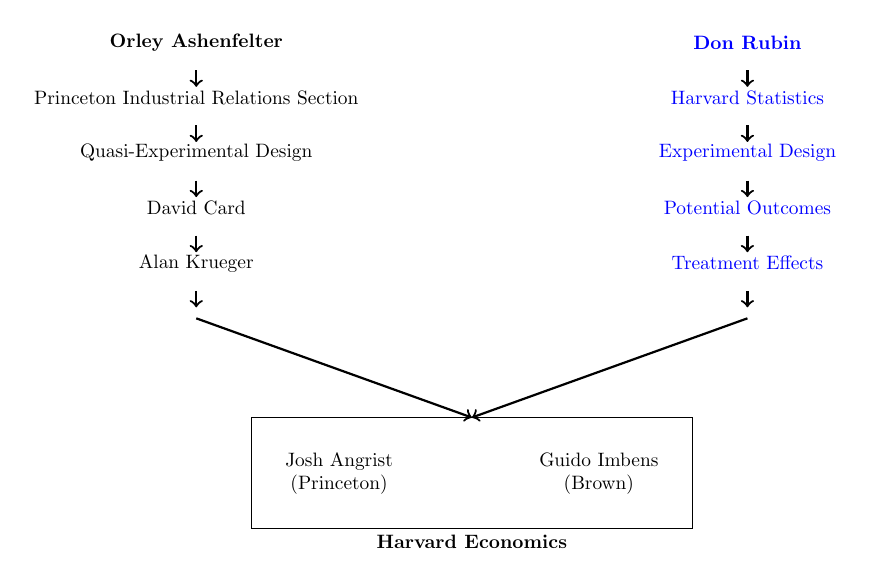
\begin{tikzpicture}[scale=0.7, every node/.style={scale=0.7}]
% Orley Ashenfelter Stream
\node at (-5,6) {\textbf{Orley Ashenfelter}};
\draw[->, thick] (-5,5.5) -- (-5,5.2);
\node at (-5,5) {Princeton Industrial Relations Section};
\draw[->, thick] (-5,4.5) -- (-5,4.2);
\node at (-5,4) {Quasi-Experimental Design};
\draw[->, thick] (-5,3.5) -- (-5,3.2);
\node at (-5,3) {David Card};
\draw[->, thick] (-5,2.5) -- (-5,2.2);
\node at (-5,2) {Alan Krueger};
\draw[->, thick] (-5,1.5) -- (-5,1.2);

% Don Rubin Stream
\begin{scope}[every node/.append style={text=blue}]
\node at (5,6) {\textbf{Don Rubin}};
\draw[->, thick] (5,5.5) -- (5,5.2);
\node at (5,5) {Harvard Statistics};
\draw[->, thick] (5,4.5) -- (5,4.2);
\node at (5,4) {Experimental Design};
\draw[->, thick] (5,3.5) -- (5,3.2);
\node at (5,3) {Potential Outcomes};
\draw[->, thick] (5,2.5) -- (5,2.2);
\node at (5,2) {Treatment Effects};
\draw[->, thick] (5,1.5) -- (5,1.2);
\end{scope}

% Arrow from Orley Ashenfelter and Don Rubin streams to bottom rectangle
\draw[->, thick] (-5,1) -- (0,-0.8);
\draw[->, thick] (5,1) -- (0,-0.8);

% Bottom Rectangle
\node[draw, minimum width=8cm, minimum height=2cm, anchor=north] at (0,-0.8) {
    \begin{tabular}{c}
        Josh Angrist \\
        (Princeton)
    \end{tabular}
    \hspace{2cm}
    \begin{tabular}{c}
        Guido Imbens \\
        (Brown)
    \end{tabular}
};
\node[anchor=north] at (0,-2.8) {\textbf{Harvard Economics}};

\end{tikzpicture}

\end{frame}

\begin{frame}{Confounding}

\begin{itemize}

\item One of the main ways that the "design" part of this branch focused on was "adjusting for observables" that could be violating independence
\item This work goes back a long way -- even to Yule in the 19th century who used regression with controls
\item But we want to now give a more modern, comprehensive review of this material
\item We will use graphs to help us better understand when we can eliminate selection bias by simply including observables controls, or what is called "unconfoundedness", "ignorability", "selection on observables" or "exogeneity"

\end{itemize}

\end{frame}



\subsection{Graph notation}

\begin{frame}{Judea Pearl, 2011 Turing Award winner}

  \begin{figure}
    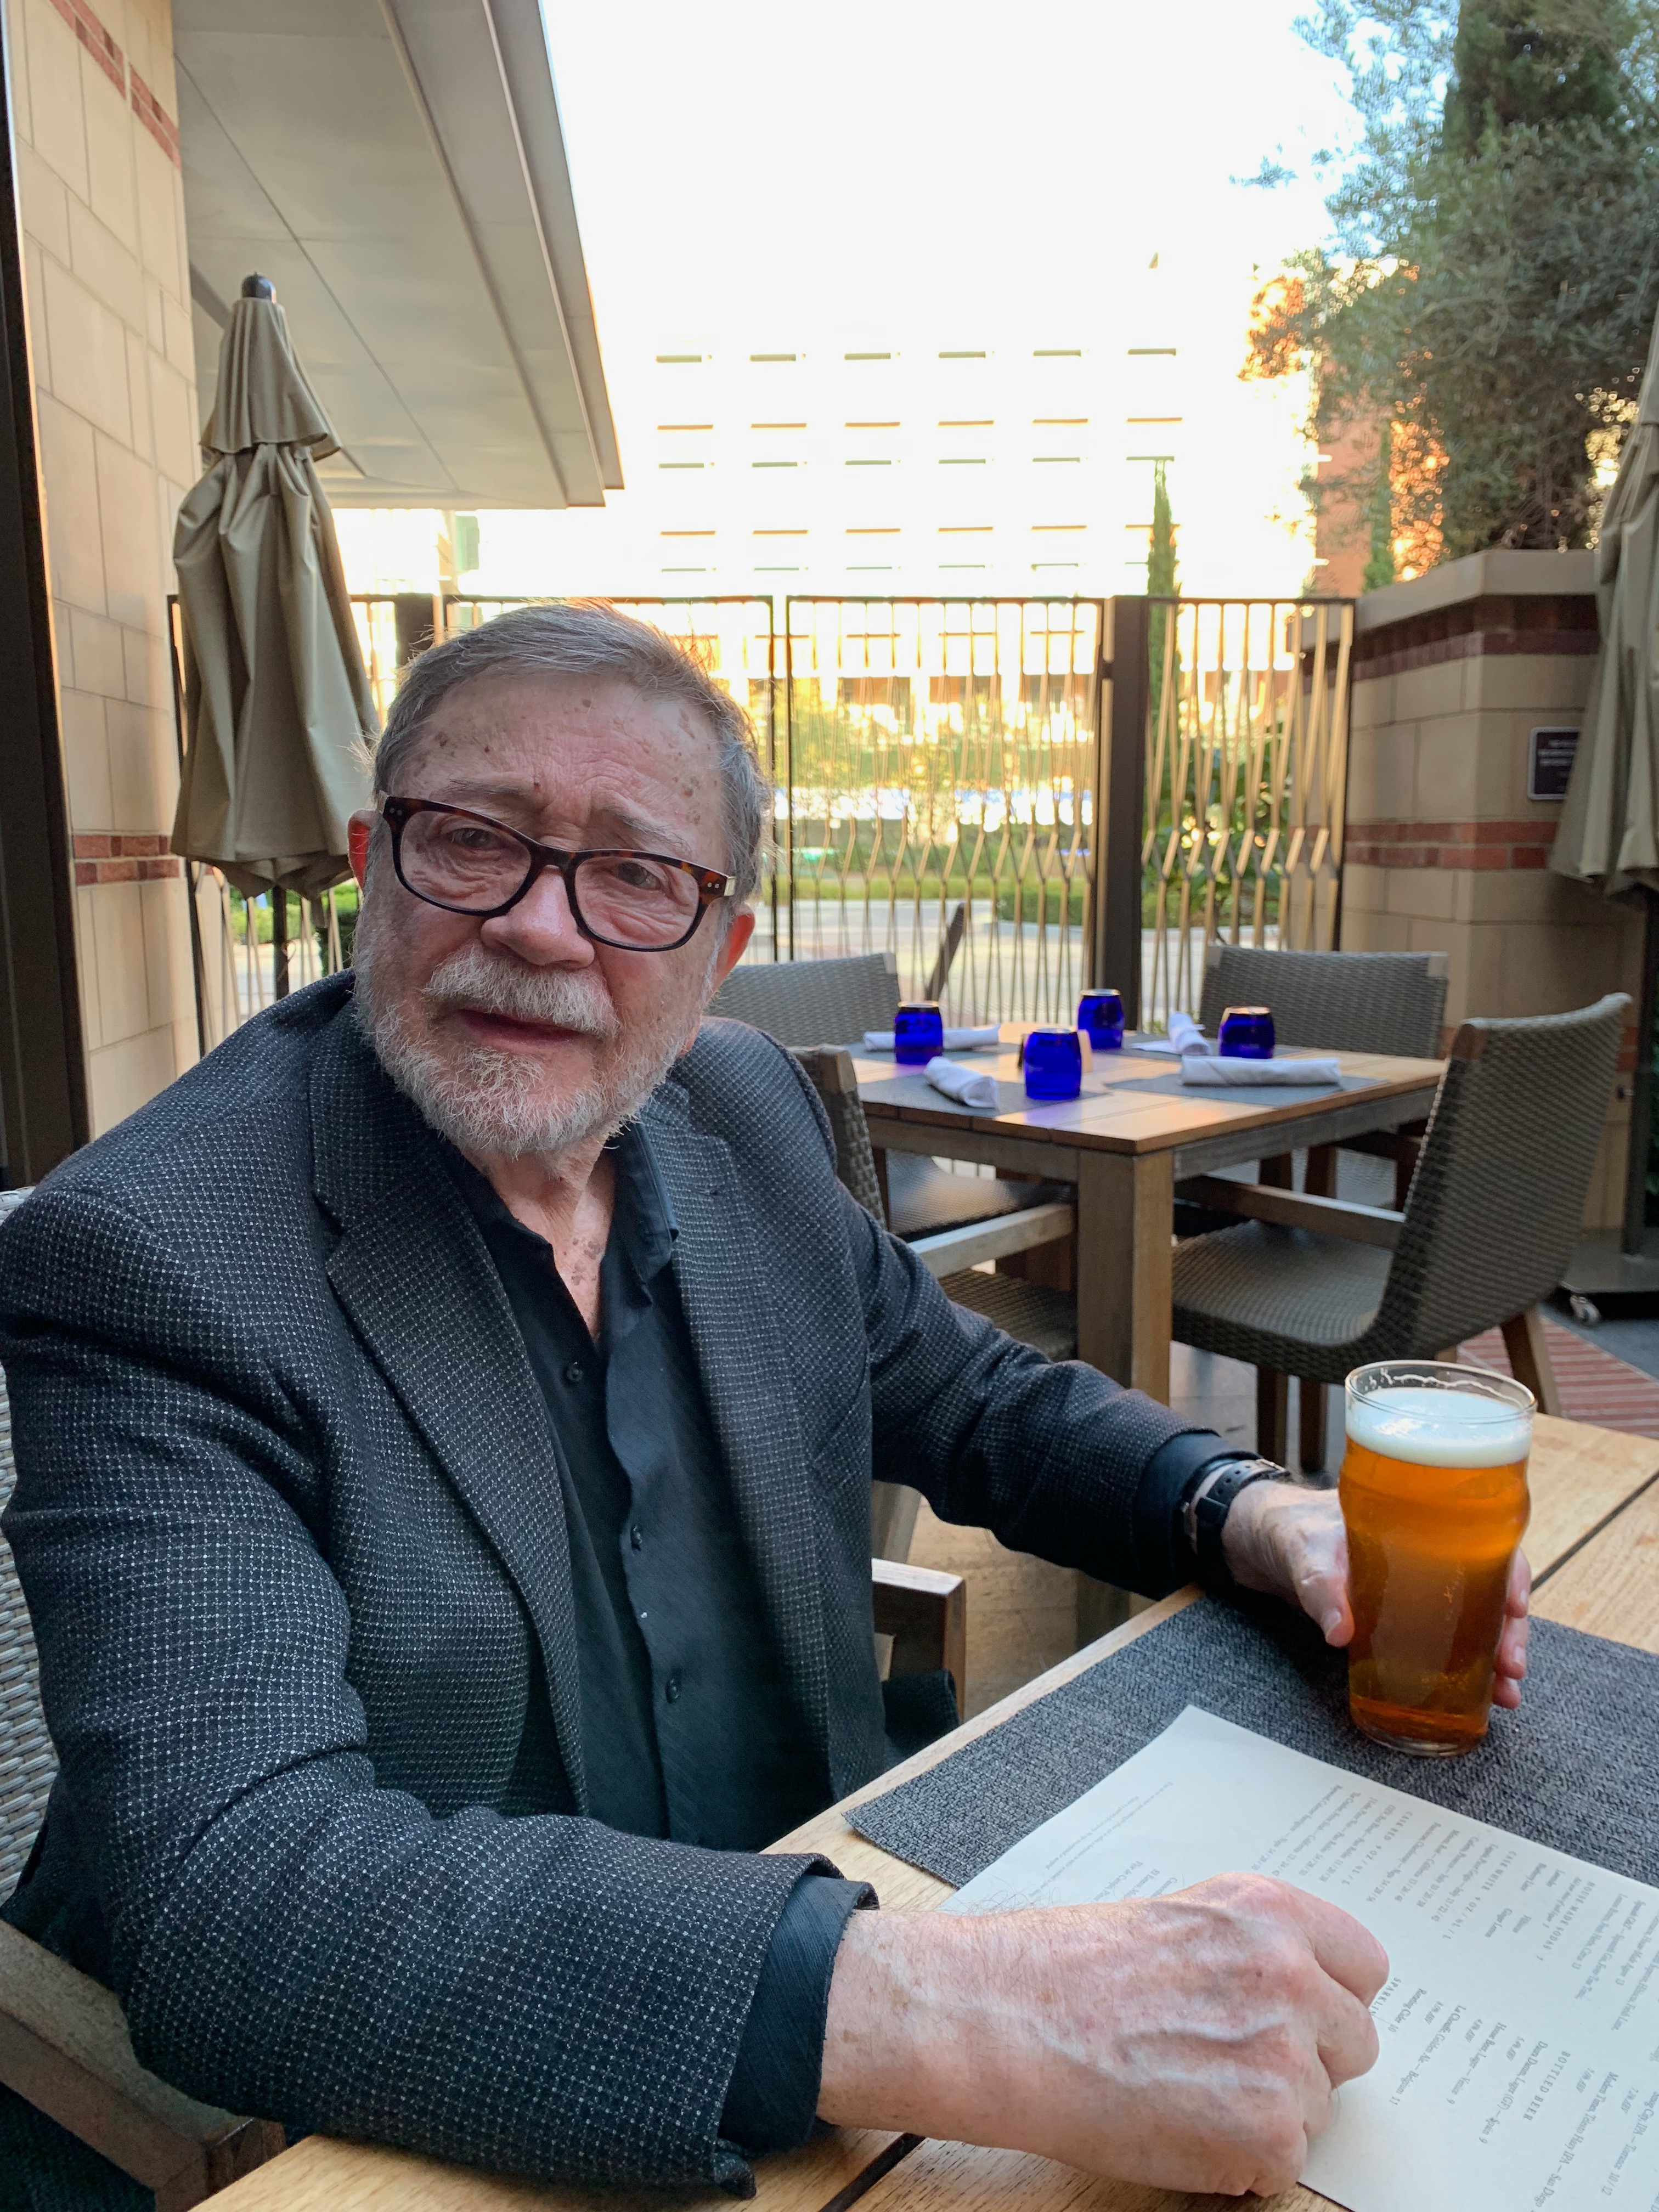
\includegraphics[scale=0.05]{./lecture_includes/pearl_ipa.jpg}
  \end{figure}

\end{frame}


\begin{frame}{Judea Pearl and DAGs}


  \begin{itemize}
    \item Judea Pearl and colleagues in Artificial Intelligence at UCLA developed directed acyclic graphs (DAGs) modeling to create a formalized causal inference methodology
    \item The letters mean this:
    	\begin{itemize}
	\item \textbf{D}: Directed.  This is a reference to graph theory.  Direct edges represent causal pathways from one variable to another
	\item \textbf{A}: Acyclic.  This means that the causal pathway only moves in one direction.  No loops or feedbacks. Limits its ability to represent many things in economics (e.g., reverse causality, simultaneous equations)
	\item \textbf{G}: Graphs. And this is also a reference to graph theory.  These are represented with a system of nodes and arrows
	\end{itemize}
    \item We'll use these to understand selection on observables ("unconfoundedness") and instrumental variables
  \end{itemize}

\end{frame}






\begin{frame}{Causal model}

  \begin{itemize}
  \item DAGs use the prior information you have about the treatment assignment and the determinants of the outcome to model the various channels (both direct and through backdoors) that the treatment causes the outcome
	\item If your knowledge of the DAG is correct, then identification of average treatment effects becomes straightforward -- but there are few ways to ``prove'' the DAG so their popularity among economists has been met with skepticism
	\item But for the selection of covariates to be used in any method that controls for covariates, they are indispensable 
    \item Consider the following diagram representing the returns to education with simplified confounders
  \end{itemize}

\end{frame}


\begin{frame}[plain]

  \begin{center}
    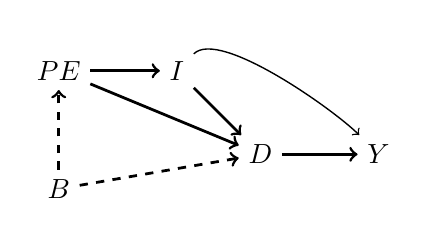
\begin{tikzpicture}[node distance=1.5cm]
      % nodes %
      \node[text centered] (d) {$D$};
      \node[right of = d, text centered] (y) {$Y$};
      \node[above left of = d, text centered] (i) {$I$};
      \node[left of = i, text centered] (pe) {$PE$};
      \node[below of = pe, text centered] (b) {$B$};
      % edges %
      \draw[->, line width= 1] (d) -- (y);
      \draw[->, line width= 1,] (i) -- (d);
      \draw[->, line width= 1,] (pe) -- (i);
      \draw[->, line width= 1,] (pe) -- (d);
      \draw[->, line width= 1, dashed] (b) -- (pe);
      \draw[->, line width= 1, dashed] (b) -- (d);
      \draw[->, line width= .5] (i) to [out=45,in=135, looseness=0.5] (y);
    \end{tikzpicture}
  \end{center}

  \bigskip
  \begin{itemize}
    \item $B$ is a \textbf{parent} of $PE$ and $D$
    \item $PE$ and $D$ are \textbf{descendants} of $B$
    \item There is a \textbf{direct (causal) path} from $D$ to $Y$
    \item There is a \textbf{mediated (causal) path} from $B$ to $Y$ through $D$
    \item There are a lot of \textbf{paths} from $PE$ to $Y$ but none are direct, and some go ``downstream'' but others go ``upstream''
  \end{itemize}
\end{frame}





\begin{frame}{Creating your DAG}

	\begin{itemize}
	\item Create a DAG that is a reasonable and honest approximation of $D$ and $Y$ parents (confounders) as well as direct and indirect effects of $D$ on $Y$
	\item Where there is uncertainty, you have to acknowledge that in the DAG, and where there are beliefs, you acknowledge that too
	\item We get ideas for DAGs from theory, models, observation, experience, prior studies, intuition, as well as conversations with domain experts
	\end{itemize}

\end{frame}


\begin{frame}{DAGs Pre-Analysis Stage}

	\begin{itemize}
	\item DAGs are meant to represent the truth about treatment assignment mechanisms and selection for the units in \emph{your data} 
	\item But creating the DAGs after you collect the data may be cheating as you're able to draw the DAG based simply on what you have rather than what is true
	\item What determines the treatment in \emph{your dataset} may be different from what determines in someone else's even if the topic is the same
	\item You'll need to spend time before your projects understanding why units in your data enrolled in the treatment -- this isn't something you do after your get the data 
	\end{itemize}
\end{frame}




% 	\item The DAG is a reasonable approximation of all common parents of $D$ and $Y$ (confounders) and direct relationships between $D and $Y$


\subsection{Backdoor criterion}


\begin{frame}{Confounding}

  \begin{itemize}
  	\item The covariates you need to control for under unconfoundedness are called \textbf{confounders}, as confounders create backdoor paths from treatment to outcome
          \item Confounders create selection bias \\

          \begin{center}
            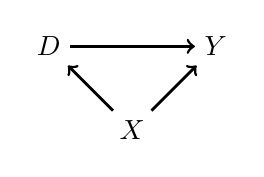
\begin{tikzpicture}
              [node distance=1.5cm]
              % nodes %
              \node[text centered] (d) {$D$};
              \node[below right of = d, text centered] (x) {$X$};
              \node[above right of = x, text centered] (y) {$Y$};

              % edges %
              \draw[->, line width= 1] (d) -- (y);
              \draw[->, line width= 1] (x) -- (d);
              \draw[->, line width= 1] (x) -- (y);
            \end{tikzpicture}
          \end{center}

          \item Our knowledge about this will enable us to select the correct covariates (but not necessarily the correct specification)
          \item Let's look at \texttt{confounders.do} in our shared labs (/Labs/DAGs)
  \end{itemize}
\end{frame}

\begin{frame}{Backdoor Paths}

  \begin{itemize}
    \item Confounding creates \textbf{backdoor paths} between treatment and outcome ($D\leftarrow X\rightarrow Y$) -- i.e., spurious correlations
		\begin{itemize}
		\item Distinct from something called a collider path ($D \rightarrow X \leftarrow Y$)
		\item Distinct from something called a mediator path ($D \rightarrow X \rightarrow Y$)
		\end{itemize}
    \item We can ``block'' any particular backdoor path by conditioning on variable $X$ so long as it is not a collider (visualized here with a square over X)

  \end{itemize}

  \begin{center}
    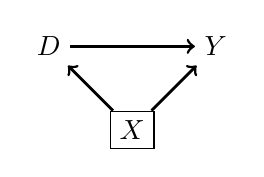
\begin{tikzpicture}
      [node distance=1.5cm]
      % nodes %
      \node[text centered] (d) {$D$};
      \node[below right of = d, text centered, rectangle, draw, thin] (x) {$X$};
      \node[above right of = x, text centered] (y) {$Y$};

      % edges %
      \draw[->, line width= 1] (d) -- (y);
      \draw[->, line width= 1] (x) -- (d);
      \draw[->, line width= 1] (x) -- (y);
    \end{tikzpicture}
  \end{center}

\end{frame}

\begin{frame}{Backdoor Paths}

  \begin{itemize}
    \item Once we condition on $X$, we can calculate average differences in $Y$ by treatment status to obtain an estimate of an aggregate causal parameter
    \item There are many methods for doing this and we cover them today -- regression, matching, stratification, weights
    \item But all of them at their fundamental level are calculating simple differences in mean outcomes for given values of $X$ and then taking weighted averages

  \end{itemize}

  \begin{center}
    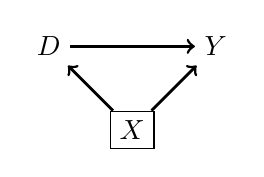
\begin{tikzpicture}
      [node distance=1.5cm]
      % nodes %
      \node[text centered] (d) {$D$};
      \node[below right of = d, text centered, rectangle, draw, thin] (x) {$X$};
      \node[above right of = x, text centered] (y) {$Y$};

      % edges %
      \draw[->, line width= 1] (d) -- (y);
      \draw[->, line width= 1] (x) -- (d);
      \draw[->, line width= 1] (x) -- (y);
    \end{tikzpicture}
  \end{center}

\end{frame}


\begin{frame}{Backdoor Paths}

  \begin{itemize}

	\item When all backdoor paths from $D$ to $Y$ are blocked, then the only remaining path between $D$ to $Y$ is the causal path
	\item We call this satisfying the backdoor criterion using Pearl's DAG terminology, and we call it unconfoundedness using Rubin's potential outcomes terminology (which I'll discuss later)

  \end{itemize}

  \begin{center}
    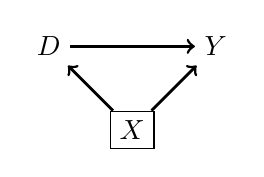
\begin{tikzpicture}
      [node distance=1.5cm]
      % nodes %
      \node[text centered] (d) {$D$};
      \node[below right of = d, text centered, rectangle, draw, thin] (x) {$X$};
      \node[above right of = x, text centered] (y) {$Y$};

      % edges %
      \draw[->, line width= 1] (d) -- (y);
      \draw[->, line width= 1] (x) -- (d);
      \draw[->, line width= 1] (x) -- (y);
    \end{tikzpicture}
  \end{center}

\end{frame}








\begin{frame}{Backdoor criterion}


  \begin{block}{Backdoor criterion}
    Conditioning on $X$ satisfies the backdoor criterion with respect to $(D,Y)$ directed path if:
    \begin{enumerate}
      \item All backdoor paths are blocked by $X$
      \item No element of $X$ is a collider

    \end{enumerate}

    
  \end{block}
       Conditioning on a non-collider is sufficient to closing a backdoor path even if it's been opened by conditioning on a collider, so just be sure to close a backdoor path if you opened it with a collider


\end{frame}

\begin{frame}{What control strategy meets the backdoor criterion?}
  \begin{itemize}
    \item List all backdoor paths from $D$ to $Y$. I'll wait.

          \begin{center}
            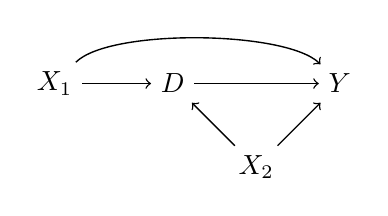
\begin{tikzpicture}
              [node distance=1.5cm]
              % nodes %
              \node[text centered,rectangle,thin] (x1) {$X_1$};
              \node[right of = x1, text centered] (d) {$D$};
              \node[below right of = d, text centered] (x2) {$X_2$};
              \node[above right of = x2, text centered] (y) {$Y$};

              % edges %
              \draw[->, line width= .5] (x1) -- (d);
              \draw[->, line width= .5] (d) -- (y);
              \draw[->, line width= .5] (x2) -- (d);
              \draw[->, line width= .5] (x2) -- (y);
              \draw[->, line width= .5] (x1) to [out=45,in=135, looseness=0.5] (y);
            \end{tikzpicture}
          \end{center}

    \item What are the necessary and sufficient set of controls which will satisfy the backdoor criterion?
  \end{itemize}

  \framebreak




\end{frame}


\begin{frame}{What if you have an unobservable?}


  \begin{itemize}
    \item List all the backdoor paths from $D$ to $Y$.

          \begin{center}
            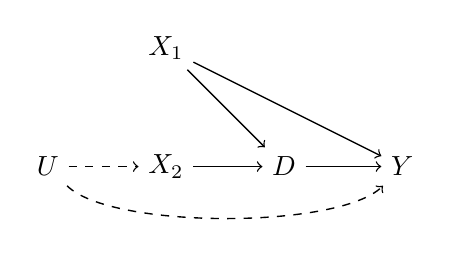
\begin{tikzpicture}
              [node distance=1.5cm]
              % nodes %
              \node[text centered] (u) {$U$};
              \node[right of = u, text centered] (x2) {$X_2$};
              \node[above of = x2, text centered] (x1) {$X_1$};
              \node[right of = x2, text centered] (d) {$D$};
              \node[right of = d, text centered] (y) {$Y$};

              % edges %
              \draw[->, line width= .5, dashed] (u) -- (x2);
              \draw[->, line width= .5] (x2) -- (d);
              \draw[->, line width= .5] (x1) -- (d);
              \draw[->, line width= .5] (x1) -- (y);
              \draw[->, line width= .5] (d) -- (y);
              \draw[->, line width= .5, dashed] (u) to [out=-45,in=-135, looseness=0.5] (y);
            \end{tikzpicture}
          \end{center}

    \item What are the necessary and sufficient set of controls which will satisfy the backdoor criterion?
    \item What about the unobserved variable, $U$?
  \end{itemize}

  \framebreak


\end{frame}

\begin{frame}{Multiple strategies}


  \begin{center}
    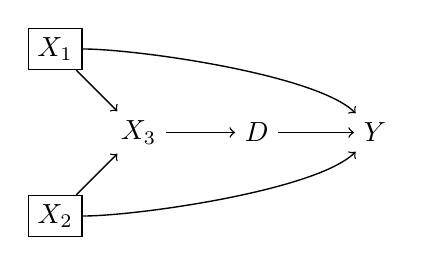
\begin{tikzpicture}
      [node distance=1.5cm, text centered]
      % nodes %
      \node[] (x3) {$X_3$};
      \node[above left of = x3,rectangle,draw,thin] (x1) {$X_1$};
      \node[below left of = x3,rectangle,draw,thin] (x2) {$X_2$};
      \node[right of = x3] (d) {$D$};
      \node[right of = d] (y) {$Y$};

      % edges %
      \draw[->, line width= .5] (x1) -- (x3);
      \draw[->, line width= .5] (x2) -- (x3);
      \draw[->, line width= .5] (x1) to [out=0,in=135, looseness=0.5] (y);
      \draw[->, line width= .5] (x2) to [out=0,in=-135, looseness=0.5] (y);
      \draw[->, line width= .5] (x3) -- (d);
      \draw[->, line width= .5] (d) -- (y);
    \end{tikzpicture}

    \vspace{1em}

    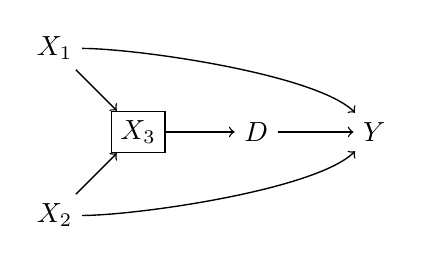
\begin{tikzpicture}
      [node distance=1.5cm, text centered]
      % nodes %
      \node[rectangle,draw,thin] (x3) {$X_3$};
      \node[above left of = x3] (x1) {$X_1$};
      \node[below left of = x3] (x2) {$X_2$};
      \node[right of = x3] (d) {$D$};
      \node[right of = d] (y) {$Y$};

      % edges %
      \draw[->, line width= .5] (x1) -- (x3);
      \draw[->, line width= .5] (x2) -- (x3);
      \draw[->, line width= .5] (x1) to [out=0,in=135, looseness=0.5] (y);
      \draw[->, line width= .5] (x2) to [out=0,in=-135, looseness=0.5] (y);
      \draw[->, line width= .5] (x3) -- (d);
      \draw[->, line width= .5] (d) -- (y);
    \end{tikzpicture}
  \end{center}

  \begin{itemize}
  \tiny
    \item Conditioning on the common causes, $X_1$ and $X_2$, is sufficient but so is conditioning on $X_3$
    \item See \texttt{confounder_multiple.do} for differences in variance -- overcontrolling is more precise
  \end{itemize}
\end{frame}






\subsection{Collider bias}

\begin{frame}{Collider bias}

\begin{itemize}
\item Backdoor paths can remain open in covariate adjustment strategies through two ways:
	\begin{enumerate}
	\item You did not close the path because you did not condition on the confounder
	\item Your conditioning variable opened up a previously closed backdoor path because on that path the variable was a \textbf{collider}
	\end{enumerate}
\item Colliders are ``bad controls'' which when you control for them, \emph{create} new previously non-existent spurious correlations (not commonly discussed, even in economics)
\item This is the risk of blindly controlling for variables -- you may inadvertently include bad or irrelevant controls
\end{itemize}

\end{frame}


\begin{frame}{Example 1: Movie stars}

  \alert{Important}: Since unconditioned colliders block back-door paths, what exactly does conditioning on a collider do? Let's illustrate with a fun example and some made-up data\\
  \begin{itemize}
    \item \underline{CNN.com} headline: Megan Fox voted worst -- but sexiest -- actress of 2009 \myurlshort{http://marquee.blogs.cnn.com/2009/12/30/megan-fox-voted-worst-but-sexiest-actress-of-2009/}{(link)}
    \item Are these two things actually negatively correlated in the world?
    \item Assume talent and beauty are independent, but each causes someone to become a movie star.  What's the correlation between talent and beauty for a sample of movie stars compared to the population as a whole (stars and non-stars)?
  \end{itemize}

\end{frame}


\begin{frame}{Movie star DAG}

Imagine casting directors pick movie stars based on talent and beauty

  \begin{center}
    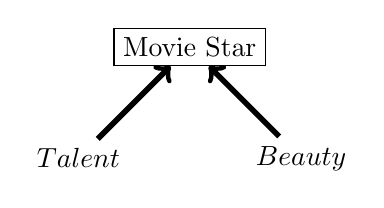
\begin{tikzpicture}
      [node distance=2cm, text centered]

      %nodes
      \node[text centered,draw,rectangle,thin] (x) {Movie Star};
      \node[below left of = x] (u1) {$Talent$};
      \node[below right of = x] (u2) {$Beauty$};

      % edges %
      \draw[->, line width= 2] (u1) -- (x);
      \draw[->, line width= 2] (u2) -- (x);
    \end{tikzpicture}
  \end{center}

Talent and beauty can become correlated even though they are independent; see \texttt{moviestar.do} or \texttt{moviestar.R}


\end{frame}

\begin{frame}[shrink=20,plain]

  \begin{figure}
    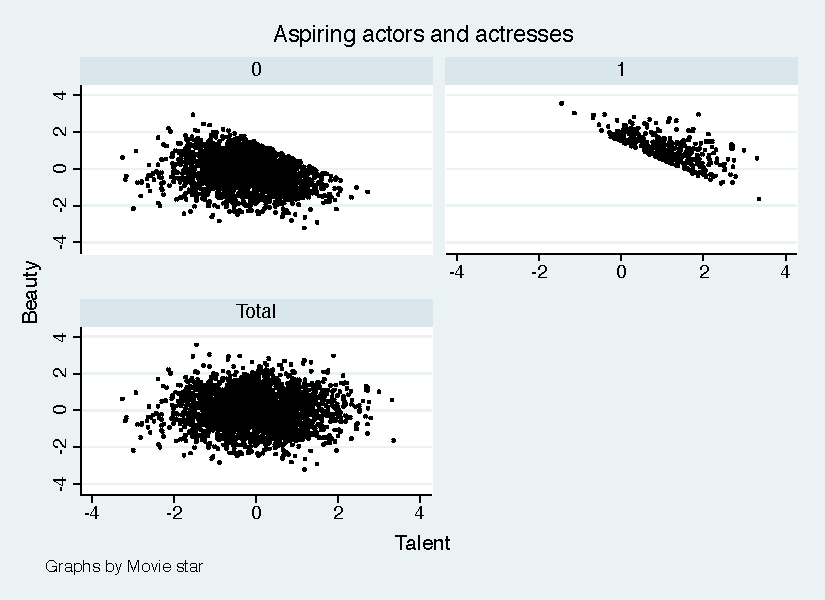
\includegraphics[height=9cm]{./lecture_includes/beauty_collider.pdf}
    \caption{Top left figure: Non-star sample scatter plot of beauty (vertical axis) and talent (horizontal axis). Top right right figure: Star sample scatter plot of beauty and talent.  Bottom left figure: Entire (stars and non-stars combined) sample scatter plot of beauty and talent.}
  \end{figure}
\end{frame}

\begin{frame}{Sample selection?}

\begin{itemize}
\item Notice that this is clear when we are focused on sample selection
\item But even a regression that included ``star'' would create the issue:$$beauty_i = \alpha + \delta talent_i + \beta star_i + \varepsilon_i$$
\item It's not just sample selection 
\end{itemize}

\end{frame}


\begin{frame}{Example 2: Discrimination}

  \begin{itemize}
    \item Let's look at another example: very common for think tanks and journalists to say that the gender gap in earnings disappears once you control for occupation.
    \item But what if occupation is a collider, which it could be in a model with occupational sorting
    \item Then controlling for occupation in a wage regression searching for discrimination can lead to all kinds of crazy results \emph{even in a simulation where we explicitly design there to be discrimination}
  \end{itemize}

\end{frame}

\begin{frame}{DAG}

  \begin{center}
    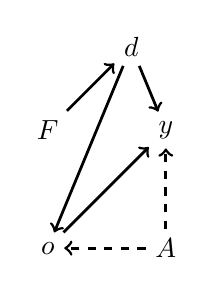
\begin{tikzpicture}
      [node distance=1.5cm]
      % nodes %
      \node[text centered] (f) {$F$};
      \node[above right of = f, text centered] (d) {$d$};
      \node[right of = f] (y) {$y$};
      \node[below  of = f, text centered] (o) {$o$};
      \node[right of = o, text centered] (a) {$A$};

      % edges %
      \draw[->, line width= 1] (f) -- (d);
      \draw[->, line width= 1] (d) -- (o);
      \draw[->, line width= 1, dashed] (a) -- (o);

      \draw[->, line width= 1] (d) -- (y);
      \draw[->, line width= 1] (o) -- (y);
      \draw[->, line width= 1, dashed] (a) -- (y);

    \end{tikzpicture}
  \end{center}

  $F$ is female, $d$ is discrimination, $o$ is occupation, $y$ is earnings and $A$ is ability. Dashed lines mean the variable cannot be observed. Note, by design, being a female has no effect on earnings or occupation, and has no relationship with ability. So earnings is coming through discrimination, occupation, and ability.

\end{frame}


\begin{frame}[plain]

  \begin{center}
    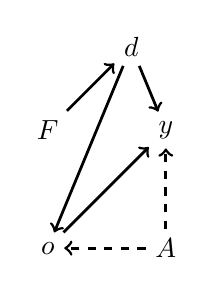
\begin{tikzpicture}
      [node distance=1.5cm]
      % nodes %
      \node[text centered] (f) {$F$};
      \node[above right of = f, text centered] (d) {$d$};
      \node[right of = f] (y) {$y$};
      \node[below  of = f, text centered] (o) {$o$};
      \node[right of = o, text centered] (a) {$A$};

      % edges %
      \draw[->, line width= 1] (f) -- (d);
      \draw[->, line width= 1] (d) -- (o);
      \draw[->, line width= 1, dashed] (a) -- (o);

      \draw[->, line width= 1] (d) -- (y);
      \draw[->, line width= 1] (o) -- (y);
      \draw[->, line width= 1, dashed] (a) -- (y);

    \end{tikzpicture}
  \end{center}


  Mediation and Backdoor paths

  \begin{enumerate}

    \item $d$ $\rightarrow o \rightarrow y$
    \item $d$ $\rightarrow o \leftarrow A \rightarrow y$
  \end{enumerate}

\end{frame}


\begin{frame}[plain, shrink=20]

  \begin{table}[htbp]\centering
    \scriptsize
    \caption{Regressions illustrating collider bias with simulated gender disparity}
    \begin{center}
      \begin{tabular}{l*{3}{c}}
        \toprule
        \multicolumn{1}{l}{Covariates: }&
        \multicolumn{1}{c}{\textbf{Unbiased combined effect}}&
        \multicolumn{1}{c}{\textbf{Biased }}&
        \multicolumn{1}{c}{\textbf{Unbiased wage effect only}}\\
        \midrule
        Female                     & -3.074*** & 0.601*** & -0.994*** \\
                                   & (0.000)   & (0.000)  & (0.000)   \\
        Occupation                 &           & 1.793*** & 0.991***  \\
                                   &           & (0.000)  & (0.000)   \\
        Ability                    &           &          & 2.017***  \\
                                   &           &          & (0.000)   \\
        \\
        \midrule
        N                          & 10,000    & 10,000   & 10,000    \\
        Mean of dependent variable & 0.45      & 0.45     & 0.45      \\
        \bottomrule
      \end{tabular}
    \end{center}
  \end{table}

  \begin{itemize}
    \item Recall we designed there to be a discrimination coefficient of -1
    \item If we do not control for occupation, then we get the combined effect of $d \rightarrow o \rightarrow y$ and $d  \rightarrow y$
    \item Because it seems intuitive to control for occupation, notice column 2 - the sign flips!
    \item We are only able to isolate the direct causal effect by conditioning on ability and occupation, but ability is unobserved
  \end{itemize}

\end{frame}

\begin{frame}[allowframebreaks,plain]

  \begin{itemize}
    \item \textbf{Colliders can be outcomes (and often those are the ones)}
          \begin{itemize}
            \item There is only one backdoor path from $D$ to $Y$

                  \begin{center}
                    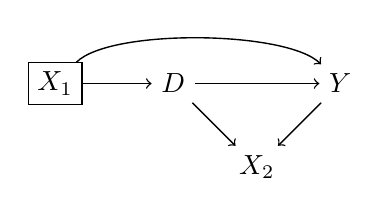
\begin{tikzpicture}
                      [node distance=1.5cm]
                      % nodes %
                      \node[text centered,draw,rectangle,thin] (x1) {$X_1$};
                      \node[right of = x1, text centered] (d) {$D$};
                      \node[below right of = d, text centered] (x2) {$X_2$};
                      \node[above right of = x2, text centered] (y) {$Y$};

                      % edges %
                      \draw[->, line width= .5] (x1) -- (d);
                      \draw[->, line width= .5] (d) -- (y);
                      \draw[->, line width= .5] (d) -- (x2);
                      \draw[->, line width= .5] (y) -- (x2);
                      \draw[->, line width= .5] (x1) to [out=45,in=135, looseness=0.5] (y);
                    \end{tikzpicture}
                  \end{center}
                  

            \item Conditioning on $X_1$ blocks the backdoor path


            \item But what if we also condition on $X_2$?

                  \begin{center}
                    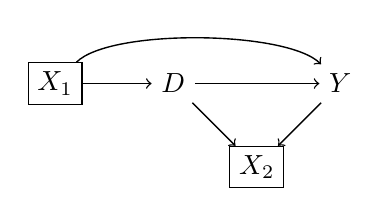
\begin{tikzpicture}
                      [node distance=1.5cm]
                      % nodes %
                      \node[text centered,draw,rectangle,thin] (x1) {$X_1$};
                      \node[right of = x1, text centered] (d) {$D$};
                      \node[below right of = d, draw, rectangle, text centered] (x2) {$X_2$};
                      \node[above right of = x2, text centered] (y) {$Y$};

                      % edges %
                      \draw[->, line width= .5] (x1) -- (d);
                      \draw[->, line width= .5] (d) -- (y);
                      \draw[->, line width= .5] (d) -- (x2);
                      \draw[->, line width= .5] (y) -- (x2);
                      \draw[->, line width= .5] (x1) to [out=45,in=135, looseness=0.5] (y);
                    \end{tikzpicture}
                  \end{center}

            \item Conditioning on $X_2$ opens up a new path, creating new spurious correlations between $D$ and $Y$ 
          \end{itemize}

          \framebreak


    \item \textbf{Colliders could be pre-treatment covariates (called M-bias because it looks like an M)}
          \begin{itemize}
            \item Name the backdoor paths.  Is it open or closed?

                  \begin{center}
                    \begin{tikzpicture}
                      [node distance=1.5cm, text centered]
                      % nodes %
                      \node[] (x) {$X$};
                      \node[above left of = x] (u1) {$U_1$};
                      \node[below left of = x] (u2) {$U_2$};
                      \node[right of = x] (d) {$D$};
                      \node[right of = d] (y) {$Y$};

                      % edges %
                      \draw[->, line width= .5, dashed] (u1) -- (x);
                      \draw[->, line width= .5, dashed] (u2) -- (x);
                      \draw[->, line width= .5, dashed] (u1) to [out=0,in=135, looseness=0.5] (y);
                      \draw[->, line width= .5, dashed] (u2) to [out=0,in=-135, looseness=0.5] (d);
                      \draw[->, line width= .5] (d) -- (y);
                    \end{tikzpicture}
                  \end{center}

            \item But what if we condition on $X$?

                  \begin{center}
                    \begin{tikzpicture}
                      [node distance=1.5cm, text centered]
                      % nodes %
                      \node[text centered,draw,rectangle,thin] (x) {$X$};
                      \node[above left of = x] (u1) {$U_1$};
                      \node[below left of = x] (u2) {$U_2$};
                      \node[right of = x] (d) {$D$};
                      \node[right of = d] (y) {$Y$};

                      % edges %
                      \draw[->, line width= .5, dashed] (u1) -- (x);
                      \draw[->, line width= .5, dashed] (u2) -- (x);
                      \draw[->, line width= .5, dashed] (u1) to [out=0,in=135, looseness=0.5] (y);
                      \draw[->, line width= .5, dashed] (u2) to [out=0,in=-135, looseness=0.5] (d);
                      \draw[->, line width= .5] (d) -- (y);
                    \end{tikzpicture}
                  \end{center}


          \end{itemize}
  \end{itemize}
  \framebreak


\end{frame}


\begin{frame}{M-bias as collider}

  \centering
  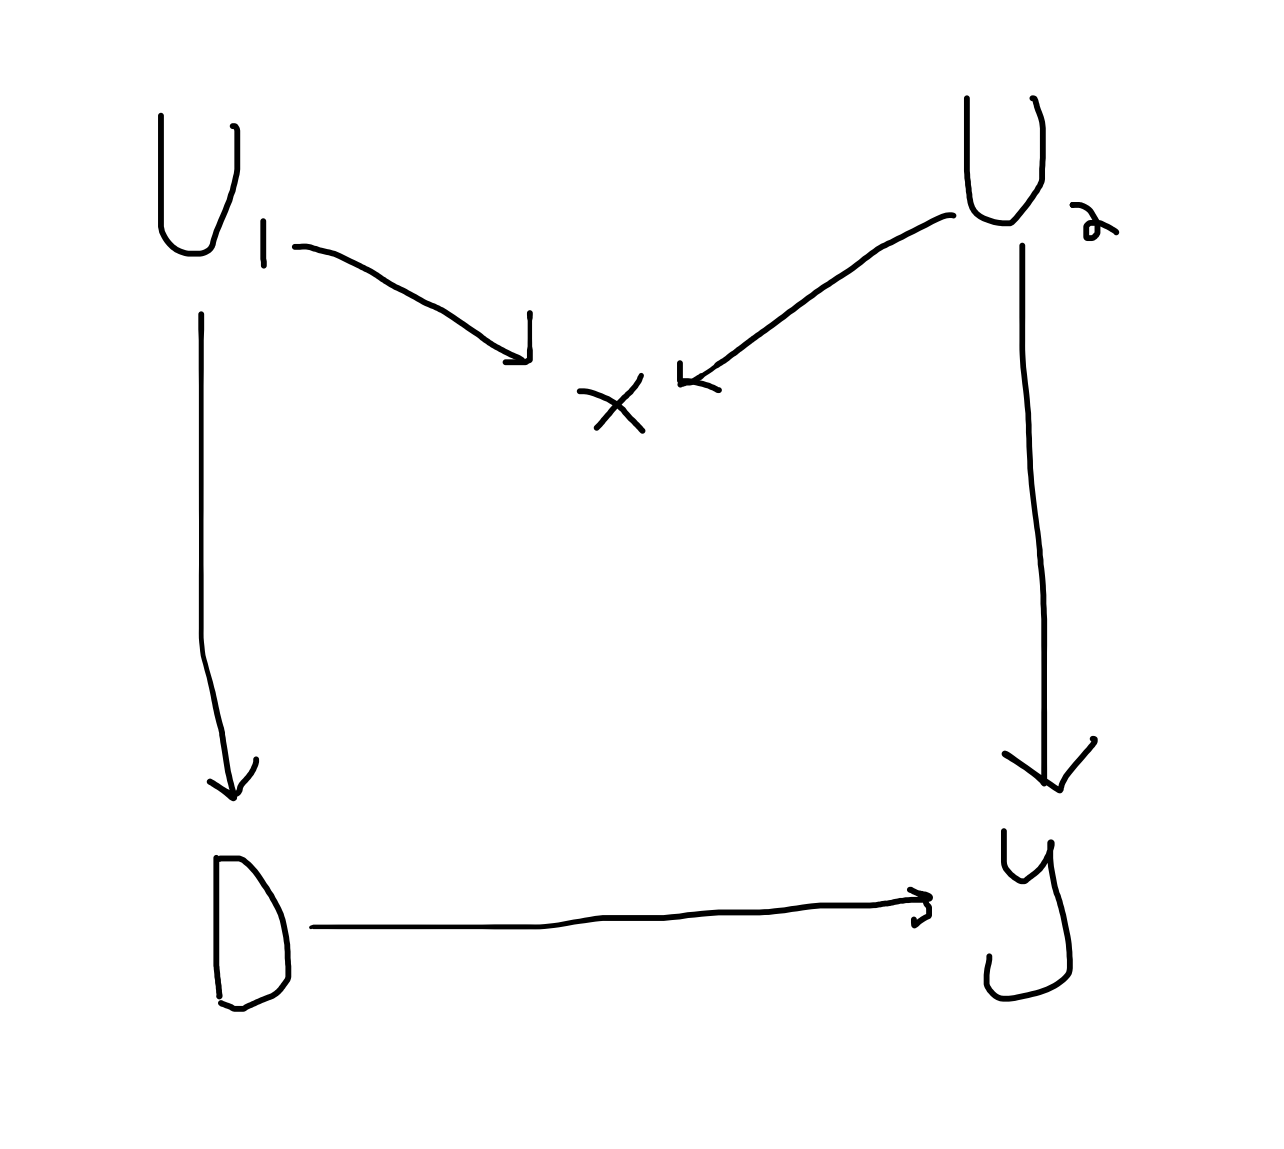
\includegraphics[height=5.8cm, width=10cm]{./lecture_includes/mbias}

\footnotesize
$X$ is pre-treatment, but if you conditioned on it, then $D\leftarrow U1 \rightarrow \mbox{X} \leftarrow U2 \rightarrow Y$ and $X$ is a collider. Colliders take strange forms, so the conditioning set \emph{must} be thoughtfully chosen based on being a strong predictor of $Y^0$, preferably based on expert knowledge and not a kitchen sink of all available regressors

\end{frame}


\begin{frame}{Testing the Validity of the DAG}

  \begin{itemize}
    \item The DAG makes testable predictions
    \item Conditional on $D$ and $I$, parental education ($PE$) should no longer be correlated with $Y$
    \item Can be hard to figure this out by hand, but software can help (e.g., Daggity.net is browser based, Causal Fusion is more advanced)
    \item Causal algorithms tend to be DAG based and are becoming popular in industry 
  \end{itemize}

  \begin{center}
    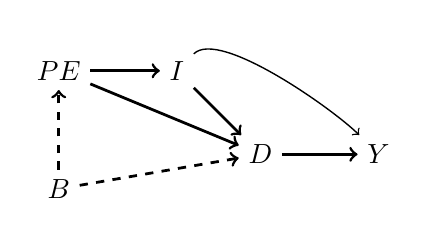
\begin{tikzpicture}[node distance=1.5cm]
      % nodes %
      \node[text centered] (d) {$D$};
      \node[right of = d, text centered] (y) {$Y$};
      \node[above left of = d, text centered] (i) {$I$};
      \node[left of = i, text centered] (pe) {$PE$};
      \node[below of = pe, text centered] (b) {$B$};
      % edges %
      \draw[->, line width= 1] (d) -- (y);
      \draw[->, line width= 1,] (i) -- (d);
      \draw[->, line width= 1,] (pe) -- (i);
      \draw[->, line width= 1,] (pe) -- (d);
      \draw[->, line width= 1, dashed] (b) -- (pe);
      \draw[->, line width= 1, dashed] (b) -- (d);
      \draw[->, line width= .5] (i) to [out=45,in=135, looseness=0.5] (y);
    \end{tikzpicture}
  \end{center}

\end{frame}




\begin{frame}{Contrast this with ordinary practices}

\begin{itemize}
\item Person attempts to ``control for omitted variable bias'' by including as many ``controls'' as possible
\item Person does not even attempt to think about treatment assignment mechanism and therefore has no idea what variables are colliders, covariates or confounders
\item Machine learning can be ``naive'' too if the large dimension of features includes unknowingly colliders
\end{itemize}

\end{frame}

\begin{frame}{}

  \begin{figure}
    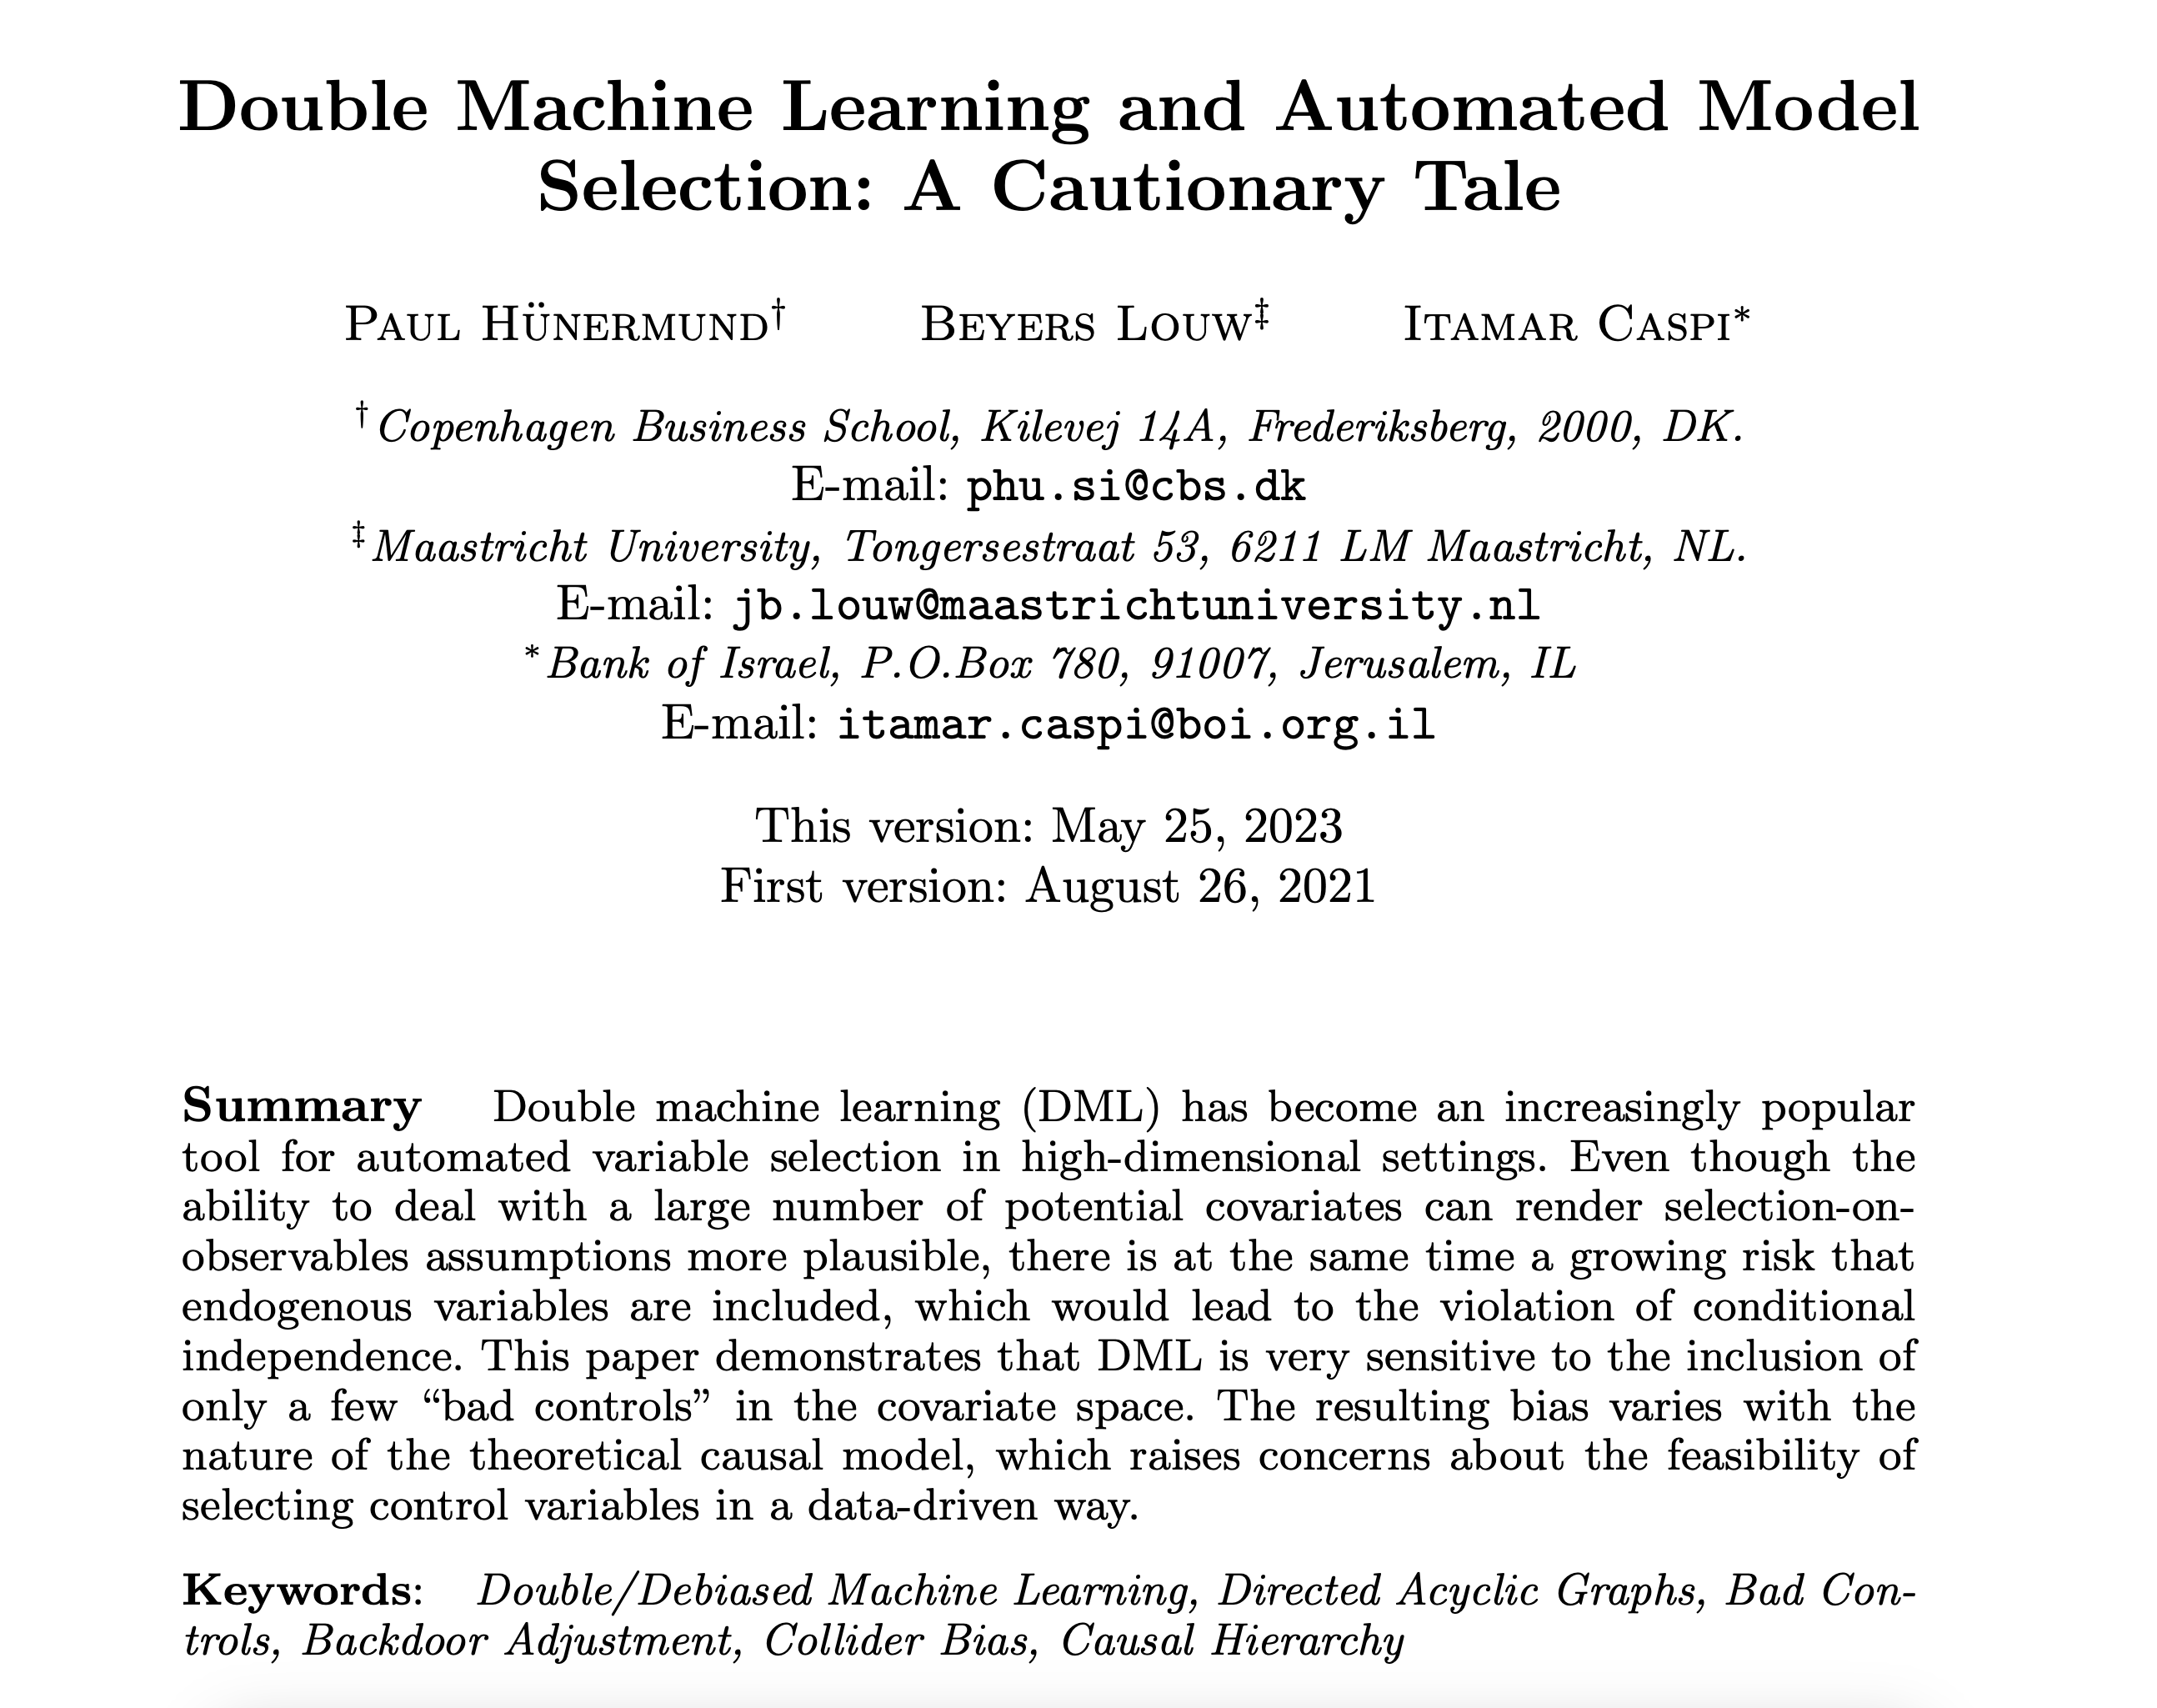
\includegraphics[scale=0.25]{./lecture_includes/paul_dml}
  \end{figure}

\end{frame}




\begin{frame}{Covariate selection without DAGs}

\begin{itemize}
\item What if you don't have a DAG you feel confident about?  
	\begin{enumerate}
	\item Include confounders that you feel pretty confident are there 
	\item Include covariates that are \emph{highly predictive} of the missing counterfactual (e.g., $Y^0$ for the ATT)
	\item Avoid outcomes (even though that still won't address M-bias colliders)
	\end{enumerate}
\item While this approach may be less formalized, you are at least reasoning about the treatment assignment mechanism as opposed to just including whatever variables you have laying around (avoid the ``kitchen sink regressions'')
\end{itemize}

\end{frame}

\begin{frame}{Falsifications as a test}

\begin{itemize}
\item Covariates should not be affected by the treatment, so examining them as falsifications can help establish the credibility of unconfoundedness
\item Imbens and Rubin (2015) suggested using the lagged outcome (pre-treatment) as a way of checking, as those have similar confounder structures
\item Falsifications too: One study questioned a finding that obesity was contagious in social networks by estimating the same model on things that cannot be contagious like acne, headaches and height and found the same things (likely confounding existed)
\end{itemize}

\end{frame}




 where the section used to sit,
% i.e. immediately before \subsection{Design Trumps Analysis}.

\section{Directed Acyclic Graphs}

\begin{frame}{Connecting today with yesterday}

\begin{itemize}
\item Day 1 we were introduced to the two defining elements of the design approach to causal inference
	\begin{enumerate}
	\item Potential Outcomes to define causal parameters (individual and average)
	\item Treatment assignment mechanism (e.g., randomization)
	\end{enumerate}
\item We also introduced the notion of ``selection bias'' and ``heterogeneous treatment effect bias''
\begin{eqnarray*}
SDO &=& ATE + \textcolor{purple}{E[Y^0|D=1]} - E[Y^0|D=0] \\
&& + (1-\pi)(ATT-ATU)
\end{eqnarray*}
\item And randomization ``deleted'' the second and third term
\end{itemize}

\end{frame}

\begin{frame}

\begin{center}
\textbf{Two design traditions}
\end{center}

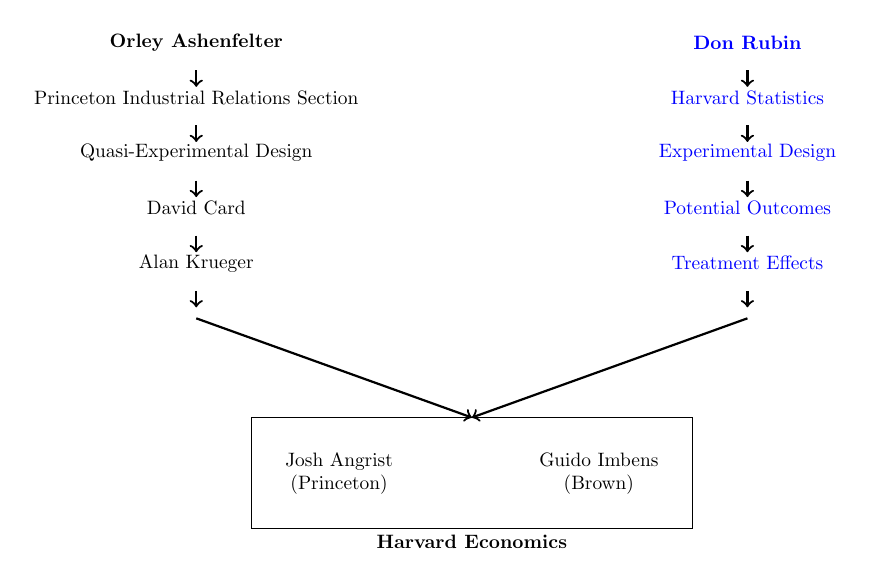
\begin{tikzpicture}[scale=0.7, every node/.style={scale=0.7}]
% Orley Ashenfelter Stream
\node at (-5,6) {\textbf{Orley Ashenfelter}};
\draw[->, thick] (-5,5.5) -- (-5,5.2);
\node at (-5,5) {Princeton Industrial Relations Section};
\draw[->, thick] (-5,4.5) -- (-5,4.2);
\node at (-5,4) {Quasi-Experimental Design};
\draw[->, thick] (-5,3.5) -- (-5,3.2);
\node at (-5,3) {David Card};
\draw[->, thick] (-5,2.5) -- (-5,2.2);
\node at (-5,2) {Alan Krueger};
\draw[->, thick] (-5,1.5) -- (-5,1.2);

% Don Rubin Stream
\begin{scope}[every node/.append style={text=blue}]
\node at (5,6) {\textbf{Don Rubin}};
\draw[->, thick] (5,5.5) -- (5,5.2);
\node at (5,5) {Harvard Statistics};
\draw[->, thick] (5,4.5) -- (5,4.2);
\node at (5,4) {Experimental Design};
\draw[->, thick] (5,3.5) -- (5,3.2);
\node at (5,3) {Potential Outcomes};
\draw[->, thick] (5,2.5) -- (5,2.2);
\node at (5,2) {Treatment Effects};
\draw[->, thick] (5,1.5) -- (5,1.2);
\end{scope}

% Arrow from Orley Ashenfelter and Don Rubin streams to bottom rectangle
\draw[->, thick] (-5,1) -- (0,-0.8);
\draw[->, thick] (5,1) -- (0,-0.8);

% Bottom Rectangle
\node[draw, minimum width=8cm, minimum height=2cm, anchor=north] at (0,-0.8) {
    \begin{tabular}{c}
        Josh Angrist \\
        (Princeton)
    \end{tabular}
    \hspace{2cm}
    \begin{tabular}{c}
        Guido Imbens \\
        (Brown)
    \end{tabular}
};
\node[anchor=north] at (0,-2.8) {\textbf{Harvard Economics}};

\end{tikzpicture}

\end{frame}

\begin{frame}{Confounding}

\begin{itemize}

\item One of the main ways that the "design" part of this branch focused on was "adjusting for observables" that could be violating independence
\item This work goes back a long way -- even to Yule in the 19th century who used regression with controls
\item But we want to now give a more modern, comprehensive review of this material
\item We will use graphs to help us better understand when we can eliminate selection bias by simply including observables controls, or what is called "unconfoundedness", "ignorability", "selection on observables" or "exogeneity"

\end{itemize}

\end{frame}



\subsection{Graph notation}

\begin{frame}{Judea Pearl, 2011 Turing Award winner}

  \begin{figure}
    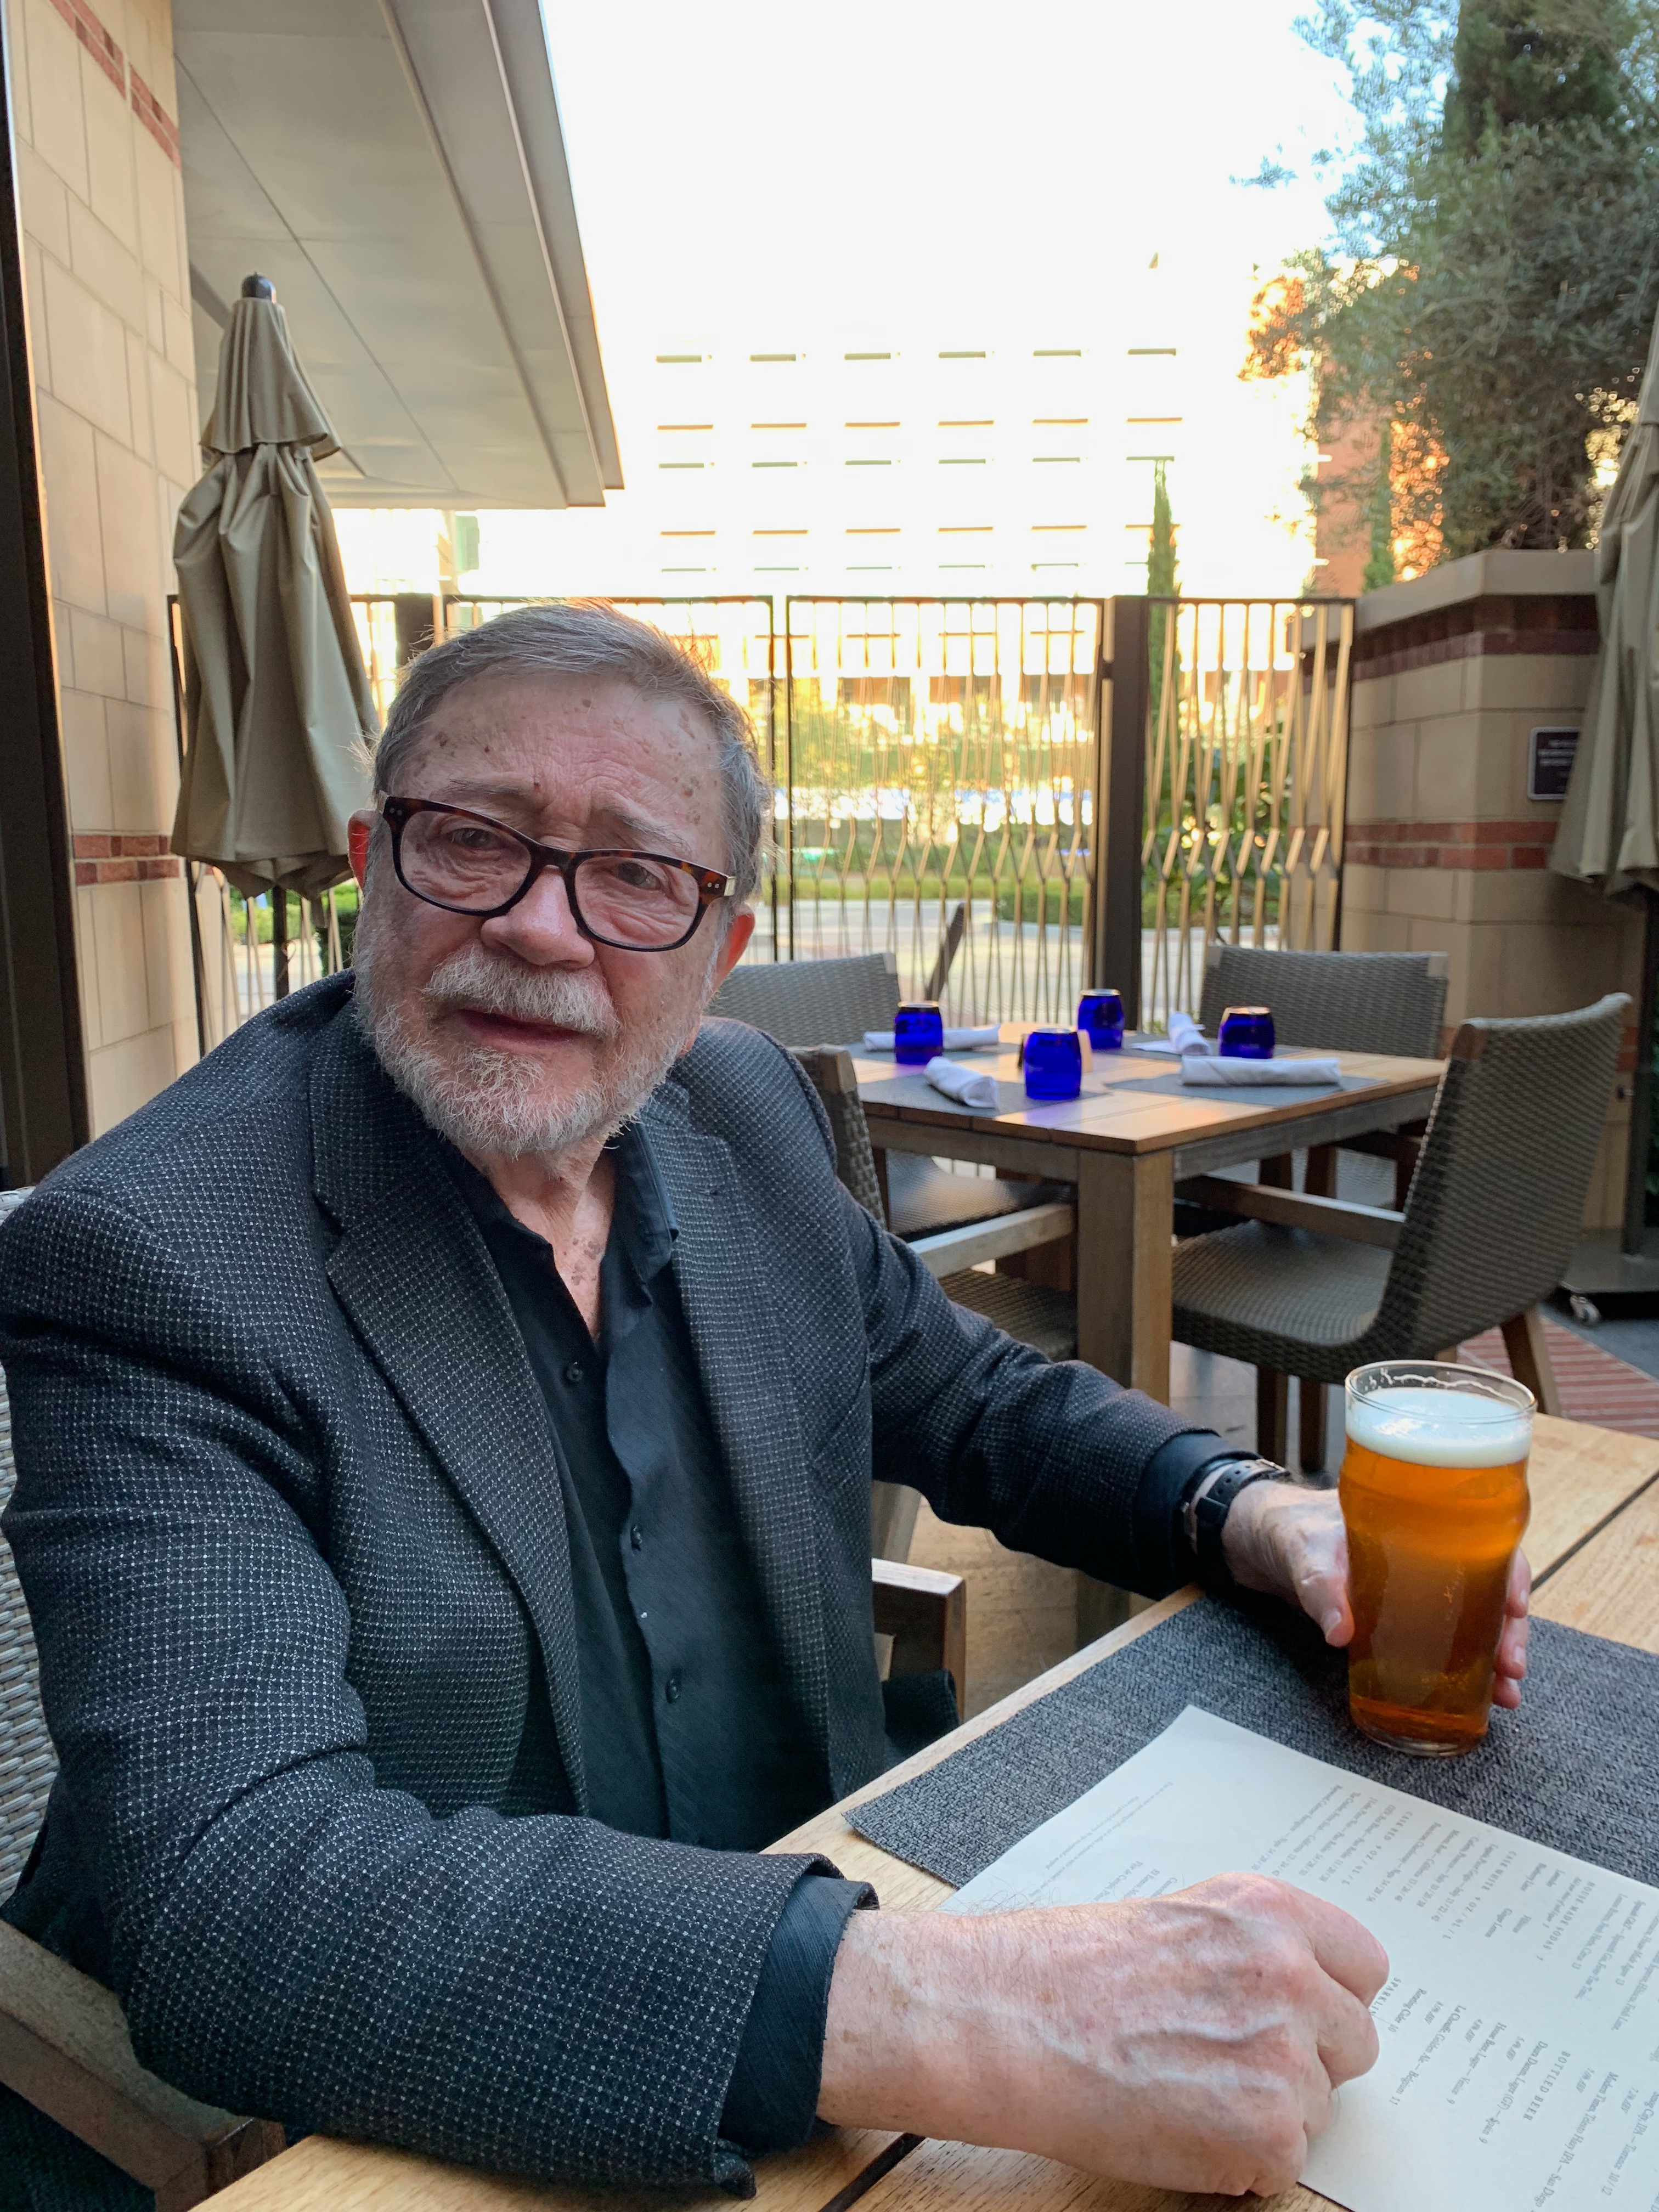
\includegraphics[scale=0.05]{./lecture_includes/pearl_ipa.jpg}
  \end{figure}

\end{frame}


\begin{frame}{Judea Pearl and DAGs}


  \begin{itemize}
    \item Judea Pearl and colleagues in Artificial Intelligence at UCLA developed directed acyclic graphs (DAGs) modeling to create a formalized causal inference methodology
    \item The letters mean this:
    	\begin{itemize}
	\item \textbf{D}: Directed.  This is a reference to graph theory.  Direct edges represent causal pathways from one variable to another
	\item \textbf{A}: Acyclic.  This means that the causal pathway only moves in one direction.  No loops or feedbacks. Limits its ability to represent many things in economics (e.g., reverse causality, simultaneous equations)
	\item \textbf{G}: Graphs. And this is also a reference to graph theory.  These are represented with a system of nodes and arrows
	\end{itemize}
    \item We'll use these to understand selection on observables ("unconfoundedness") and instrumental variables
  \end{itemize}

\end{frame}






\begin{frame}{Causal model}

  \begin{itemize}
  \item DAGs use the prior information you have about the treatment assignment and the determinants of the outcome to model the various channels (both direct and through backdoors) that the treatment causes the outcome
	\item If your knowledge of the DAG is correct, then identification of average treatment effects becomes straightforward -- but there are few ways to ``prove'' the DAG so their popularity among economists has been met with skepticism
	\item But for the selection of covariates to be used in any method that controls for covariates, they are indispensable 
    \item Consider the following diagram representing the returns to education with simplified confounders
  \end{itemize}

\end{frame}


\begin{frame}[plain]

  \begin{center}
    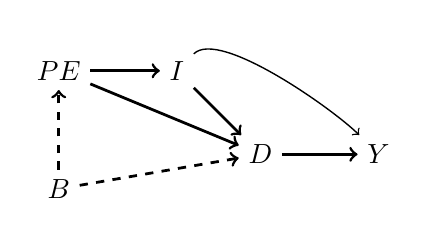
\begin{tikzpicture}[node distance=1.5cm]
      % nodes %
      \node[text centered] (d) {$D$};
      \node[right of = d, text centered] (y) {$Y$};
      \node[above left of = d, text centered] (i) {$I$};
      \node[left of = i, text centered] (pe) {$PE$};
      \node[below of = pe, text centered] (b) {$B$};
      % edges %
      \draw[->, line width= 1] (d) -- (y);
      \draw[->, line width= 1,] (i) -- (d);
      \draw[->, line width= 1,] (pe) -- (i);
      \draw[->, line width= 1,] (pe) -- (d);
      \draw[->, line width= 1, dashed] (b) -- (pe);
      \draw[->, line width= 1, dashed] (b) -- (d);
      \draw[->, line width= .5] (i) to [out=45,in=135, looseness=0.5] (y);
    \end{tikzpicture}
  \end{center}

  \bigskip
  \begin{itemize}
    \item $B$ is a \textbf{parent} of $PE$ and $D$
    \item $PE$ and $D$ are \textbf{descendants} of $B$
    \item There is a \textbf{direct (causal) path} from $D$ to $Y$
    \item There is a \textbf{mediated (causal) path} from $B$ to $Y$ through $D$
    \item There are a lot of \textbf{paths} from $PE$ to $Y$ but none are direct, and some go ``downstream'' but others go ``upstream''
  \end{itemize}
\end{frame}





\begin{frame}{Creating your DAG}

	\begin{itemize}
	\item Create a DAG that is a reasonable and honest approximation of $D$ and $Y$ parents (confounders) as well as direct and indirect effects of $D$ on $Y$
	\item Where there is uncertainty, you have to acknowledge that in the DAG, and where there are beliefs, you acknowledge that too
	\item We get ideas for DAGs from theory, models, observation, experience, prior studies, intuition, as well as conversations with domain experts
	\end{itemize}

\end{frame}


\begin{frame}{DAGs Pre-Analysis Stage}

	\begin{itemize}
	\item DAGs are meant to represent the truth about treatment assignment mechanisms and selection for the units in \emph{your data} 
	\item But creating the DAGs after you collect the data may be cheating as you're able to draw the DAG based simply on what you have rather than what is true
	\item What determines the treatment in \emph{your dataset} may be different from what determines in someone else's even if the topic is the same
	\item You'll need to spend time before your projects understanding why units in your data enrolled in the treatment -- this isn't something you do after your get the data 
	\end{itemize}
\end{frame}




% 	\item The DAG is a reasonable approximation of all common parents of $D$ and $Y$ (confounders) and direct relationships between $D and $Y$


\subsection{Backdoor criterion}


\begin{frame}{Confounding}

  \begin{itemize}
  	\item The covariates you need to control for under unconfoundedness are called \textbf{confounders}, as confounders create backdoor paths from treatment to outcome
          \item Confounders create selection bias \\

          \begin{center}
            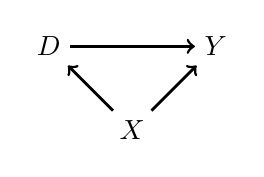
\begin{tikzpicture}
              [node distance=1.5cm]
              % nodes %
              \node[text centered] (d) {$D$};
              \node[below right of = d, text centered] (x) {$X$};
              \node[above right of = x, text centered] (y) {$Y$};

              % edges %
              \draw[->, line width= 1] (d) -- (y);
              \draw[->, line width= 1] (x) -- (d);
              \draw[->, line width= 1] (x) -- (y);
            \end{tikzpicture}
          \end{center}

          \item Our knowledge about this will enable us to select the correct covariates (but not necessarily the correct specification)
          \item Let's look at \texttt{confounders.do} in our shared labs (/Labs/DAGs)
  \end{itemize}
\end{frame}

\begin{frame}{Backdoor Paths}

  \begin{itemize}
    \item Confounding creates \textbf{backdoor paths} between treatment and outcome ($D\leftarrow X\rightarrow Y$) -- i.e., spurious correlations
		\begin{itemize}
		\item Distinct from something called a collider path ($D \rightarrow X \leftarrow Y$)
		\item Distinct from something called a mediator path ($D \rightarrow X \rightarrow Y$)
		\end{itemize}
    \item We can ``block'' any particular backdoor path by conditioning on variable $X$ so long as it is not a collider (visualized here with a square over X)

  \end{itemize}

  \begin{center}
    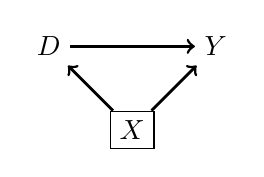
\begin{tikzpicture}
      [node distance=1.5cm]
      % nodes %
      \node[text centered] (d) {$D$};
      \node[below right of = d, text centered, rectangle, draw, thin] (x) {$X$};
      \node[above right of = x, text centered] (y) {$Y$};

      % edges %
      \draw[->, line width= 1] (d) -- (y);
      \draw[->, line width= 1] (x) -- (d);
      \draw[->, line width= 1] (x) -- (y);
    \end{tikzpicture}
  \end{center}

\end{frame}

\begin{frame}{Backdoor Paths}

  \begin{itemize}
    \item Once we condition on $X$, we can calculate average differences in $Y$ by treatment status to obtain an estimate of an aggregate causal parameter
    \item There are many methods for doing this and we cover them today -- regression, matching, stratification, weights
    \item But all of them at their fundamental level are calculating simple differences in mean outcomes for given values of $X$ and then taking weighted averages

  \end{itemize}

  \begin{center}
    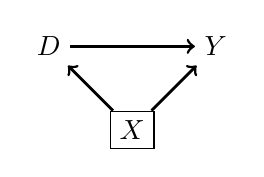
\begin{tikzpicture}
      [node distance=1.5cm]
      % nodes %
      \node[text centered] (d) {$D$};
      \node[below right of = d, text centered, rectangle, draw, thin] (x) {$X$};
      \node[above right of = x, text centered] (y) {$Y$};

      % edges %
      \draw[->, line width= 1] (d) -- (y);
      \draw[->, line width= 1] (x) -- (d);
      \draw[->, line width= 1] (x) -- (y);
    \end{tikzpicture}
  \end{center}

\end{frame}


\begin{frame}{Backdoor Paths}

  \begin{itemize}

	\item When all backdoor paths from $D$ to $Y$ are blocked, then the only remaining path between $D$ to $Y$ is the causal path
	\item We call this satisfying the backdoor criterion using Pearl's DAG terminology, and we call it unconfoundedness using Rubin's potential outcomes terminology (which I'll discuss later)

  \end{itemize}

  \begin{center}
    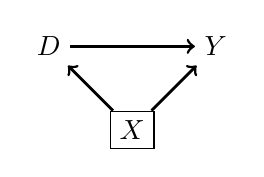
\begin{tikzpicture}
      [node distance=1.5cm]
      % nodes %
      \node[text centered] (d) {$D$};
      \node[below right of = d, text centered, rectangle, draw, thin] (x) {$X$};
      \node[above right of = x, text centered] (y) {$Y$};

      % edges %
      \draw[->, line width= 1] (d) -- (y);
      \draw[->, line width= 1] (x) -- (d);
      \draw[->, line width= 1] (x) -- (y);
    \end{tikzpicture}
  \end{center}

\end{frame}








\begin{frame}{Backdoor criterion}


  \begin{block}{Backdoor criterion}
    Conditioning on $X$ satisfies the backdoor criterion with respect to $(D,Y)$ directed path if:
    \begin{enumerate}
      \item All backdoor paths are blocked by $X$
      \item No element of $X$ is a collider

    \end{enumerate}

    
  \end{block}
       Conditioning on a non-collider is sufficient to closing a backdoor path even if it's been opened by conditioning on a collider, so just be sure to close a backdoor path if you opened it with a collider


\end{frame}

\begin{frame}{What control strategy meets the backdoor criterion?}
  \begin{itemize}
    \item List all backdoor paths from $D$ to $Y$. I'll wait.

          \begin{center}
            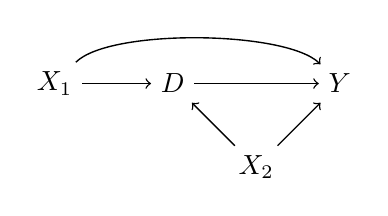
\begin{tikzpicture}
              [node distance=1.5cm]
              % nodes %
              \node[text centered,rectangle,thin] (x1) {$X_1$};
              \node[right of = x1, text centered] (d) {$D$};
              \node[below right of = d, text centered] (x2) {$X_2$};
              \node[above right of = x2, text centered] (y) {$Y$};

              % edges %
              \draw[->, line width= .5] (x1) -- (d);
              \draw[->, line width= .5] (d) -- (y);
              \draw[->, line width= .5] (x2) -- (d);
              \draw[->, line width= .5] (x2) -- (y);
              \draw[->, line width= .5] (x1) to [out=45,in=135, looseness=0.5] (y);
            \end{tikzpicture}
          \end{center}

    \item What are the necessary and sufficient set of controls which will satisfy the backdoor criterion?
  \end{itemize}

  \framebreak




\end{frame}


\begin{frame}{What if you have an unobservable?}


  \begin{itemize}
    \item List all the backdoor paths from $D$ to $Y$.

          \begin{center}
            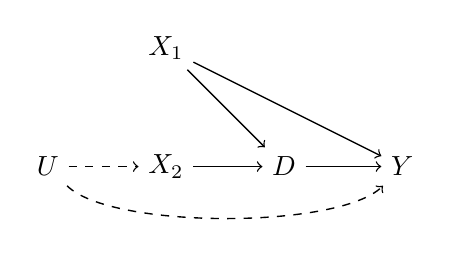
\begin{tikzpicture}
              [node distance=1.5cm]
              % nodes %
              \node[text centered] (u) {$U$};
              \node[right of = u, text centered] (x2) {$X_2$};
              \node[above of = x2, text centered] (x1) {$X_1$};
              \node[right of = x2, text centered] (d) {$D$};
              \node[right of = d, text centered] (y) {$Y$};

              % edges %
              \draw[->, line width= .5, dashed] (u) -- (x2);
              \draw[->, line width= .5] (x2) -- (d);
              \draw[->, line width= .5] (x1) -- (d);
              \draw[->, line width= .5] (x1) -- (y);
              \draw[->, line width= .5] (d) -- (y);
              \draw[->, line width= .5, dashed] (u) to [out=-45,in=-135, looseness=0.5] (y);
            \end{tikzpicture}
          \end{center}

    \item What are the necessary and sufficient set of controls which will satisfy the backdoor criterion?
    \item What about the unobserved variable, $U$?
  \end{itemize}

  \framebreak


\end{frame}

\begin{frame}{Multiple strategies}


  \begin{center}
    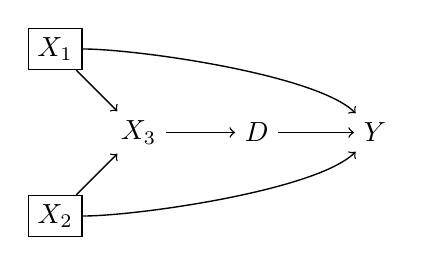
\begin{tikzpicture}
      [node distance=1.5cm, text centered]
      % nodes %
      \node[] (x3) {$X_3$};
      \node[above left of = x3,rectangle,draw,thin] (x1) {$X_1$};
      \node[below left of = x3,rectangle,draw,thin] (x2) {$X_2$};
      \node[right of = x3] (d) {$D$};
      \node[right of = d] (y) {$Y$};

      % edges %
      \draw[->, line width= .5] (x1) -- (x3);
      \draw[->, line width= .5] (x2) -- (x3);
      \draw[->, line width= .5] (x1) to [out=0,in=135, looseness=0.5] (y);
      \draw[->, line width= .5] (x2) to [out=0,in=-135, looseness=0.5] (y);
      \draw[->, line width= .5] (x3) -- (d);
      \draw[->, line width= .5] (d) -- (y);
    \end{tikzpicture}

    \vspace{1em}

    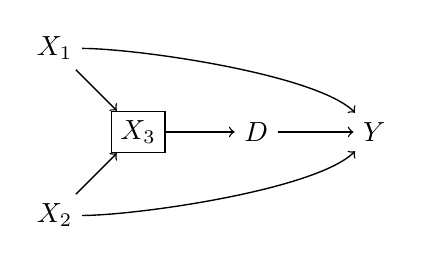
\begin{tikzpicture}
      [node distance=1.5cm, text centered]
      % nodes %
      \node[rectangle,draw,thin] (x3) {$X_3$};
      \node[above left of = x3] (x1) {$X_1$};
      \node[below left of = x3] (x2) {$X_2$};
      \node[right of = x3] (d) {$D$};
      \node[right of = d] (y) {$Y$};

      % edges %
      \draw[->, line width= .5] (x1) -- (x3);
      \draw[->, line width= .5] (x2) -- (x3);
      \draw[->, line width= .5] (x1) to [out=0,in=135, looseness=0.5] (y);
      \draw[->, line width= .5] (x2) to [out=0,in=-135, looseness=0.5] (y);
      \draw[->, line width= .5] (x3) -- (d);
      \draw[->, line width= .5] (d) -- (y);
    \end{tikzpicture}
  \end{center}

  \begin{itemize}
  \tiny
    \item Conditioning on the common causes, $X_1$ and $X_2$, is sufficient but so is conditioning on $X_3$
    \item See \texttt{confounder_multiple.do} for differences in variance -- overcontrolling is more precise
  \end{itemize}
\end{frame}






\subsection{Collider bias}

\begin{frame}{Collider bias}

\begin{itemize}
\item Backdoor paths can remain open in covariate adjustment strategies through two ways:
	\begin{enumerate}
	\item You did not close the path because you did not condition on the confounder
	\item Your conditioning variable opened up a previously closed backdoor path because on that path the variable was a \textbf{collider}
	\end{enumerate}
\item Colliders are ``bad controls'' which when you control for them, \emph{create} new previously non-existent spurious correlations (not commonly discussed, even in economics)
\item This is the risk of blindly controlling for variables -- you may inadvertently include bad or irrelevant controls
\end{itemize}

\end{frame}


\begin{frame}{Example 1: Movie stars}

  \alert{Important}: Since unconditioned colliders block back-door paths, what exactly does conditioning on a collider do? Let's illustrate with a fun example and some made-up data\\
  \begin{itemize}
    \item \underline{CNN.com} headline: Megan Fox voted worst -- but sexiest -- actress of 2009 \myurlshort{http://marquee.blogs.cnn.com/2009/12/30/megan-fox-voted-worst-but-sexiest-actress-of-2009/}{(link)}
    \item Are these two things actually negatively correlated in the world?
    \item Assume talent and beauty are independent, but each causes someone to become a movie star.  What's the correlation between talent and beauty for a sample of movie stars compared to the population as a whole (stars and non-stars)?
  \end{itemize}

\end{frame}


\begin{frame}{Movie star DAG}

Imagine casting directors pick movie stars based on talent and beauty

  \begin{center}
    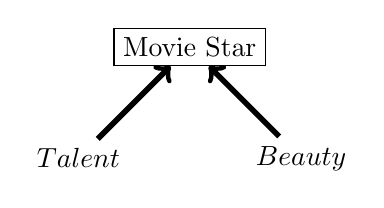
\begin{tikzpicture}
      [node distance=2cm, text centered]

      %nodes
      \node[text centered,draw,rectangle,thin] (x) {Movie Star};
      \node[below left of = x] (u1) {$Talent$};
      \node[below right of = x] (u2) {$Beauty$};

      % edges %
      \draw[->, line width= 2] (u1) -- (x);
      \draw[->, line width= 2] (u2) -- (x);
    \end{tikzpicture}
  \end{center}

Talent and beauty can become correlated even though they are independent; see \texttt{moviestar.do} or \texttt{moviestar.R}


\end{frame}

\begin{frame}[shrink=20,plain]

  \begin{figure}
    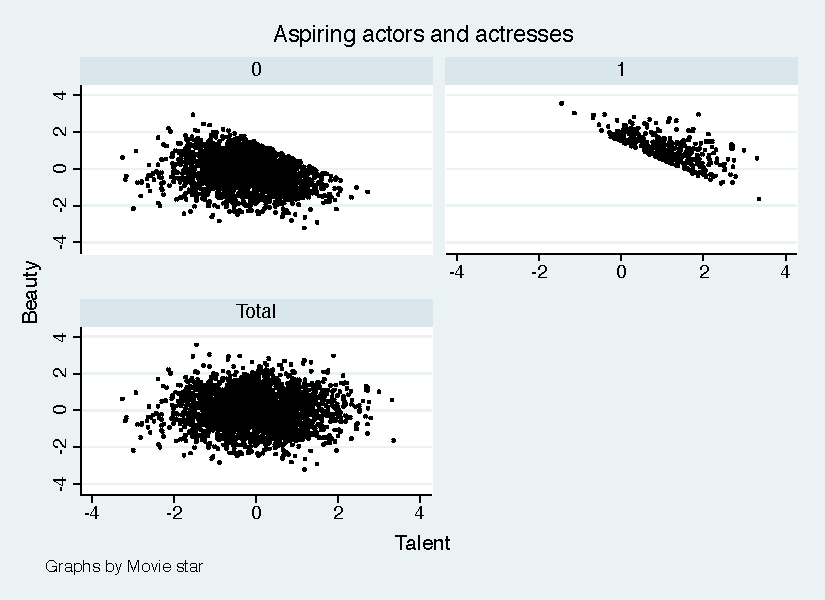
\includegraphics[height=9cm]{./lecture_includes/beauty_collider.pdf}
    \caption{Top left figure: Non-star sample scatter plot of beauty (vertical axis) and talent (horizontal axis). Top right right figure: Star sample scatter plot of beauty and talent.  Bottom left figure: Entire (stars and non-stars combined) sample scatter plot of beauty and talent.}
  \end{figure}
\end{frame}

\begin{frame}{Sample selection?}

\begin{itemize}
\item Notice that this is clear when we are focused on sample selection
\item But even a regression that included ``star'' would create the issue:$$beauty_i = \alpha + \delta talent_i + \beta star_i + \varepsilon_i$$
\item It's not just sample selection 
\end{itemize}

\end{frame}


\begin{frame}{Example 2: Discrimination}

  \begin{itemize}
    \item Let's look at another example: very common for think tanks and journalists to say that the gender gap in earnings disappears once you control for occupation.
    \item But what if occupation is a collider, which it could be in a model with occupational sorting
    \item Then controlling for occupation in a wage regression searching for discrimination can lead to all kinds of crazy results \emph{even in a simulation where we explicitly design there to be discrimination}
  \end{itemize}

\end{frame}

\begin{frame}{DAG}

  \begin{center}
    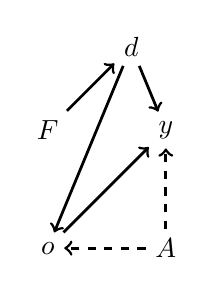
\begin{tikzpicture}
      [node distance=1.5cm]
      % nodes %
      \node[text centered] (f) {$F$};
      \node[above right of = f, text centered] (d) {$d$};
      \node[right of = f] (y) {$y$};
      \node[below  of = f, text centered] (o) {$o$};
      \node[right of = o, text centered] (a) {$A$};

      % edges %
      \draw[->, line width= 1] (f) -- (d);
      \draw[->, line width= 1] (d) -- (o);
      \draw[->, line width= 1, dashed] (a) -- (o);

      \draw[->, line width= 1] (d) -- (y);
      \draw[->, line width= 1] (o) -- (y);
      \draw[->, line width= 1, dashed] (a) -- (y);

    \end{tikzpicture}
  \end{center}

  $F$ is female, $d$ is discrimination, $o$ is occupation, $y$ is earnings and $A$ is ability. Dashed lines mean the variable cannot be observed. Note, by design, being a female has no effect on earnings or occupation, and has no relationship with ability. So earnings is coming through discrimination, occupation, and ability.

\end{frame}


\begin{frame}[plain]

  \begin{center}
    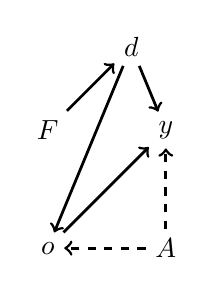
\begin{tikzpicture}
      [node distance=1.5cm]
      % nodes %
      \node[text centered] (f) {$F$};
      \node[above right of = f, text centered] (d) {$d$};
      \node[right of = f] (y) {$y$};
      \node[below  of = f, text centered] (o) {$o$};
      \node[right of = o, text centered] (a) {$A$};

      % edges %
      \draw[->, line width= 1] (f) -- (d);
      \draw[->, line width= 1] (d) -- (o);
      \draw[->, line width= 1, dashed] (a) -- (o);

      \draw[->, line width= 1] (d) -- (y);
      \draw[->, line width= 1] (o) -- (y);
      \draw[->, line width= 1, dashed] (a) -- (y);

    \end{tikzpicture}
  \end{center}


  Mediation and Backdoor paths

  \begin{enumerate}

    \item $d$ $\rightarrow o \rightarrow y$
    \item $d$ $\rightarrow o \leftarrow A \rightarrow y$
  \end{enumerate}

\end{frame}


\begin{frame}[plain, shrink=20]

  \begin{table}[htbp]\centering
    \scriptsize
    \caption{Regressions illustrating collider bias with simulated gender disparity}
    \begin{center}
      \begin{tabular}{l*{3}{c}}
        \toprule
        \multicolumn{1}{l}{Covariates: }&
        \multicolumn{1}{c}{\textbf{Unbiased combined effect}}&
        \multicolumn{1}{c}{\textbf{Biased }}&
        \multicolumn{1}{c}{\textbf{Unbiased wage effect only}}\\
        \midrule
        Female                     & -3.074*** & 0.601*** & -0.994*** \\
                                   & (0.000)   & (0.000)  & (0.000)   \\
        Occupation                 &           & 1.793*** & 0.991***  \\
                                   &           & (0.000)  & (0.000)   \\
        Ability                    &           &          & 2.017***  \\
                                   &           &          & (0.000)   \\
        \\
        \midrule
        N                          & 10,000    & 10,000   & 10,000    \\
        Mean of dependent variable & 0.45      & 0.45     & 0.45      \\
        \bottomrule
      \end{tabular}
    \end{center}
  \end{table}

  \begin{itemize}
    \item Recall we designed there to be a discrimination coefficient of -1
    \item If we do not control for occupation, then we get the combined effect of $d \rightarrow o \rightarrow y$ and $d  \rightarrow y$
    \item Because it seems intuitive to control for occupation, notice column 2 - the sign flips!
    \item We are only able to isolate the direct causal effect by conditioning on ability and occupation, but ability is unobserved
  \end{itemize}

\end{frame}

\begin{frame}[allowframebreaks,plain]

  \begin{itemize}
    \item \textbf{Colliders can be outcomes (and often those are the ones)}
          \begin{itemize}
            \item There is only one backdoor path from $D$ to $Y$

                  \begin{center}
                    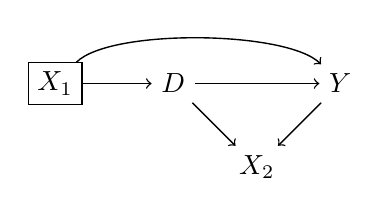
\begin{tikzpicture}
                      [node distance=1.5cm]
                      % nodes %
                      \node[text centered,draw,rectangle,thin] (x1) {$X_1$};
                      \node[right of = x1, text centered] (d) {$D$};
                      \node[below right of = d, text centered] (x2) {$X_2$};
                      \node[above right of = x2, text centered] (y) {$Y$};

                      % edges %
                      \draw[->, line width= .5] (x1) -- (d);
                      \draw[->, line width= .5] (d) -- (y);
                      \draw[->, line width= .5] (d) -- (x2);
                      \draw[->, line width= .5] (y) -- (x2);
                      \draw[->, line width= .5] (x1) to [out=45,in=135, looseness=0.5] (y);
                    \end{tikzpicture}
                  \end{center}
                  

            \item Conditioning on $X_1$ blocks the backdoor path


            \item But what if we also condition on $X_2$?

                  \begin{center}
                    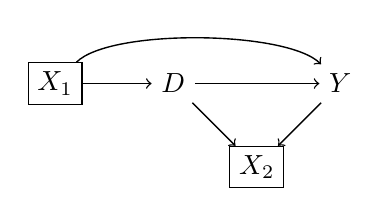
\begin{tikzpicture}
                      [node distance=1.5cm]
                      % nodes %
                      \node[text centered,draw,rectangle,thin] (x1) {$X_1$};
                      \node[right of = x1, text centered] (d) {$D$};
                      \node[below right of = d, draw, rectangle, text centered] (x2) {$X_2$};
                      \node[above right of = x2, text centered] (y) {$Y$};

                      % edges %
                      \draw[->, line width= .5] (x1) -- (d);
                      \draw[->, line width= .5] (d) -- (y);
                      \draw[->, line width= .5] (d) -- (x2);
                      \draw[->, line width= .5] (y) -- (x2);
                      \draw[->, line width= .5] (x1) to [out=45,in=135, looseness=0.5] (y);
                    \end{tikzpicture}
                  \end{center}

            \item Conditioning on $X_2$ opens up a new path, creating new spurious correlations between $D$ and $Y$ 
          \end{itemize}

          \framebreak


    \item \textbf{Colliders could be pre-treatment covariates (called M-bias because it looks like an M)}
          \begin{itemize}
            \item Name the backdoor paths.  Is it open or closed?

                  \begin{center}
                    \begin{tikzpicture}
                      [node distance=1.5cm, text centered]
                      % nodes %
                      \node[] (x) {$X$};
                      \node[above left of = x] (u1) {$U_1$};
                      \node[below left of = x] (u2) {$U_2$};
                      \node[right of = x] (d) {$D$};
                      \node[right of = d] (y) {$Y$};

                      % edges %
                      \draw[->, line width= .5, dashed] (u1) -- (x);
                      \draw[->, line width= .5, dashed] (u2) -- (x);
                      \draw[->, line width= .5, dashed] (u1) to [out=0,in=135, looseness=0.5] (y);
                      \draw[->, line width= .5, dashed] (u2) to [out=0,in=-135, looseness=0.5] (d);
                      \draw[->, line width= .5] (d) -- (y);
                    \end{tikzpicture}
                  \end{center}

            \item But what if we condition on $X$?

                  \begin{center}
                    \begin{tikzpicture}
                      [node distance=1.5cm, text centered]
                      % nodes %
                      \node[text centered,draw,rectangle,thin] (x) {$X$};
                      \node[above left of = x] (u1) {$U_1$};
                      \node[below left of = x] (u2) {$U_2$};
                      \node[right of = x] (d) {$D$};
                      \node[right of = d] (y) {$Y$};

                      % edges %
                      \draw[->, line width= .5, dashed] (u1) -- (x);
                      \draw[->, line width= .5, dashed] (u2) -- (x);
                      \draw[->, line width= .5, dashed] (u1) to [out=0,in=135, looseness=0.5] (y);
                      \draw[->, line width= .5, dashed] (u2) to [out=0,in=-135, looseness=0.5] (d);
                      \draw[->, line width= .5] (d) -- (y);
                    \end{tikzpicture}
                  \end{center}


          \end{itemize}
  \end{itemize}
  \framebreak


\end{frame}


\begin{frame}{M-bias as collider}

  \centering
  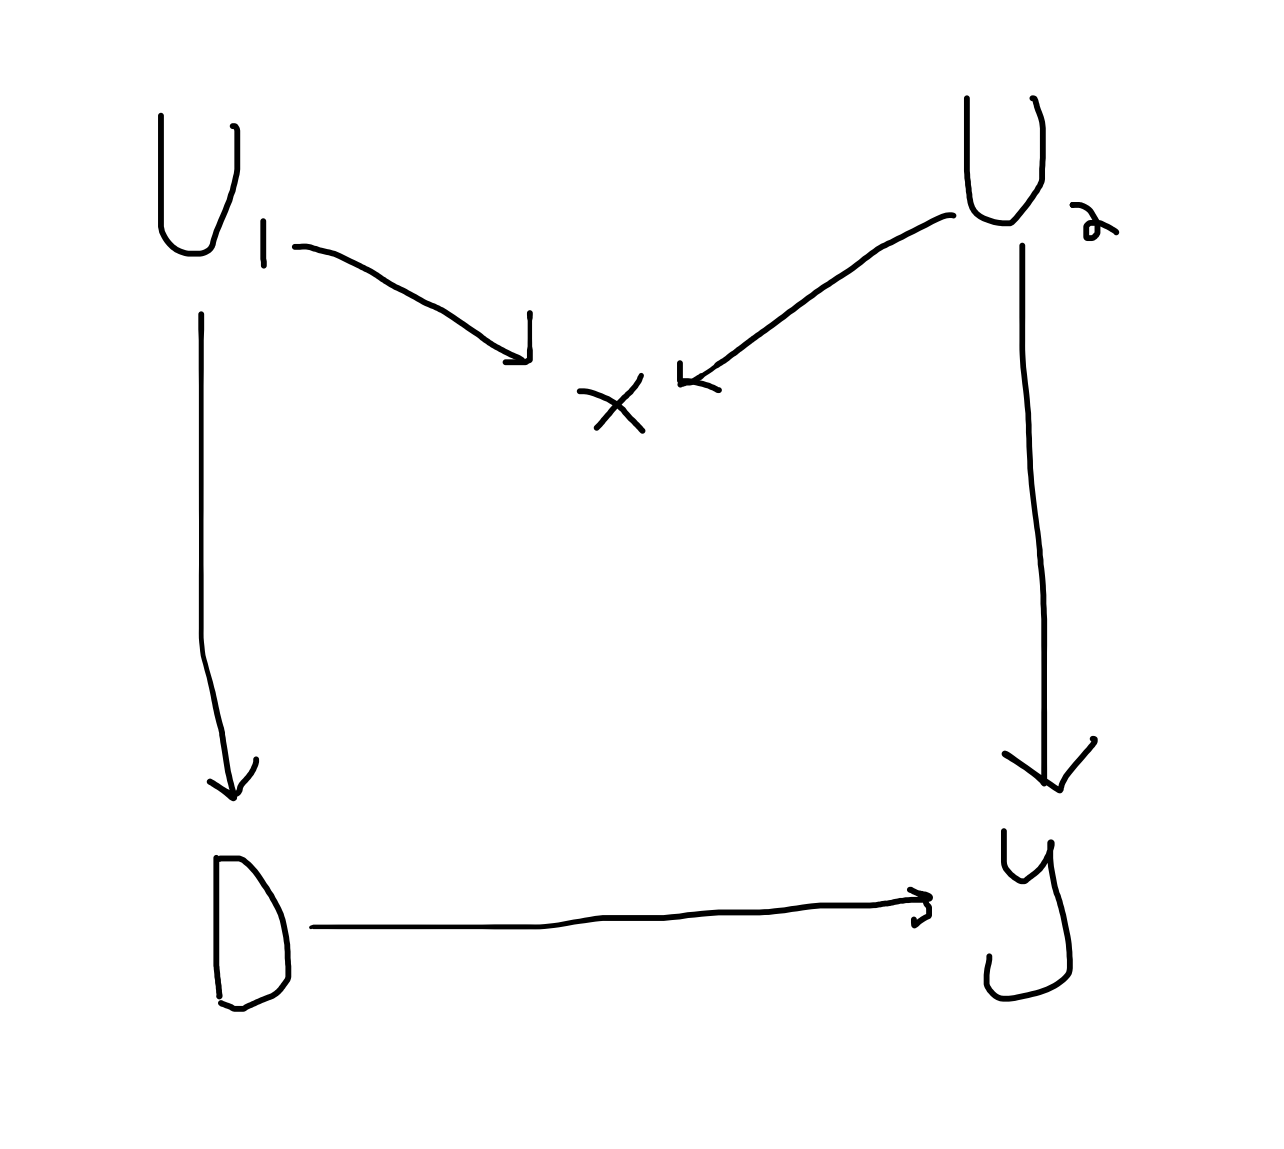
\includegraphics[height=5.8cm, width=10cm]{./lecture_includes/mbias}

\footnotesize
$X$ is pre-treatment, but if you conditioned on it, then $D\leftarrow U1 \rightarrow \mbox{X} \leftarrow U2 \rightarrow Y$ and $X$ is a collider. Colliders take strange forms, so the conditioning set \emph{must} be thoughtfully chosen based on being a strong predictor of $Y^0$, preferably based on expert knowledge and not a kitchen sink of all available regressors

\end{frame}


\begin{frame}{Testing the Validity of the DAG}

  \begin{itemize}
    \item The DAG makes testable predictions
    \item Conditional on $D$ and $I$, parental education ($PE$) should no longer be correlated with $Y$
    \item Can be hard to figure this out by hand, but software can help (e.g., Daggity.net is browser based, Causal Fusion is more advanced)
    \item Causal algorithms tend to be DAG based and are becoming popular in industry 
  \end{itemize}

  \begin{center}
    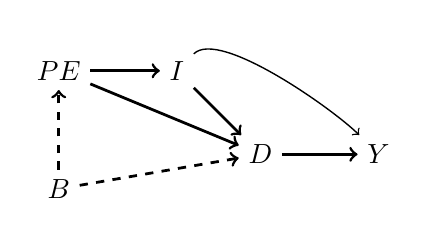
\begin{tikzpicture}[node distance=1.5cm]
      % nodes %
      \node[text centered] (d) {$D$};
      \node[right of = d, text centered] (y) {$Y$};
      \node[above left of = d, text centered] (i) {$I$};
      \node[left of = i, text centered] (pe) {$PE$};
      \node[below of = pe, text centered] (b) {$B$};
      % edges %
      \draw[->, line width= 1] (d) -- (y);
      \draw[->, line width= 1,] (i) -- (d);
      \draw[->, line width= 1,] (pe) -- (i);
      \draw[->, line width= 1,] (pe) -- (d);
      \draw[->, line width= 1, dashed] (b) -- (pe);
      \draw[->, line width= 1, dashed] (b) -- (d);
      \draw[->, line width= .5] (i) to [out=45,in=135, looseness=0.5] (y);
    \end{tikzpicture}
  \end{center}

\end{frame}




\begin{frame}{Contrast this with ordinary practices}

\begin{itemize}
\item Person attempts to ``control for omitted variable bias'' by including as many ``controls'' as possible
\item Person does not even attempt to think about treatment assignment mechanism and therefore has no idea what variables are colliders, covariates or confounders
\item Machine learning can be ``naive'' too if the large dimension of features includes unknowingly colliders
\end{itemize}

\end{frame}

\begin{frame}{}

  \begin{figure}
    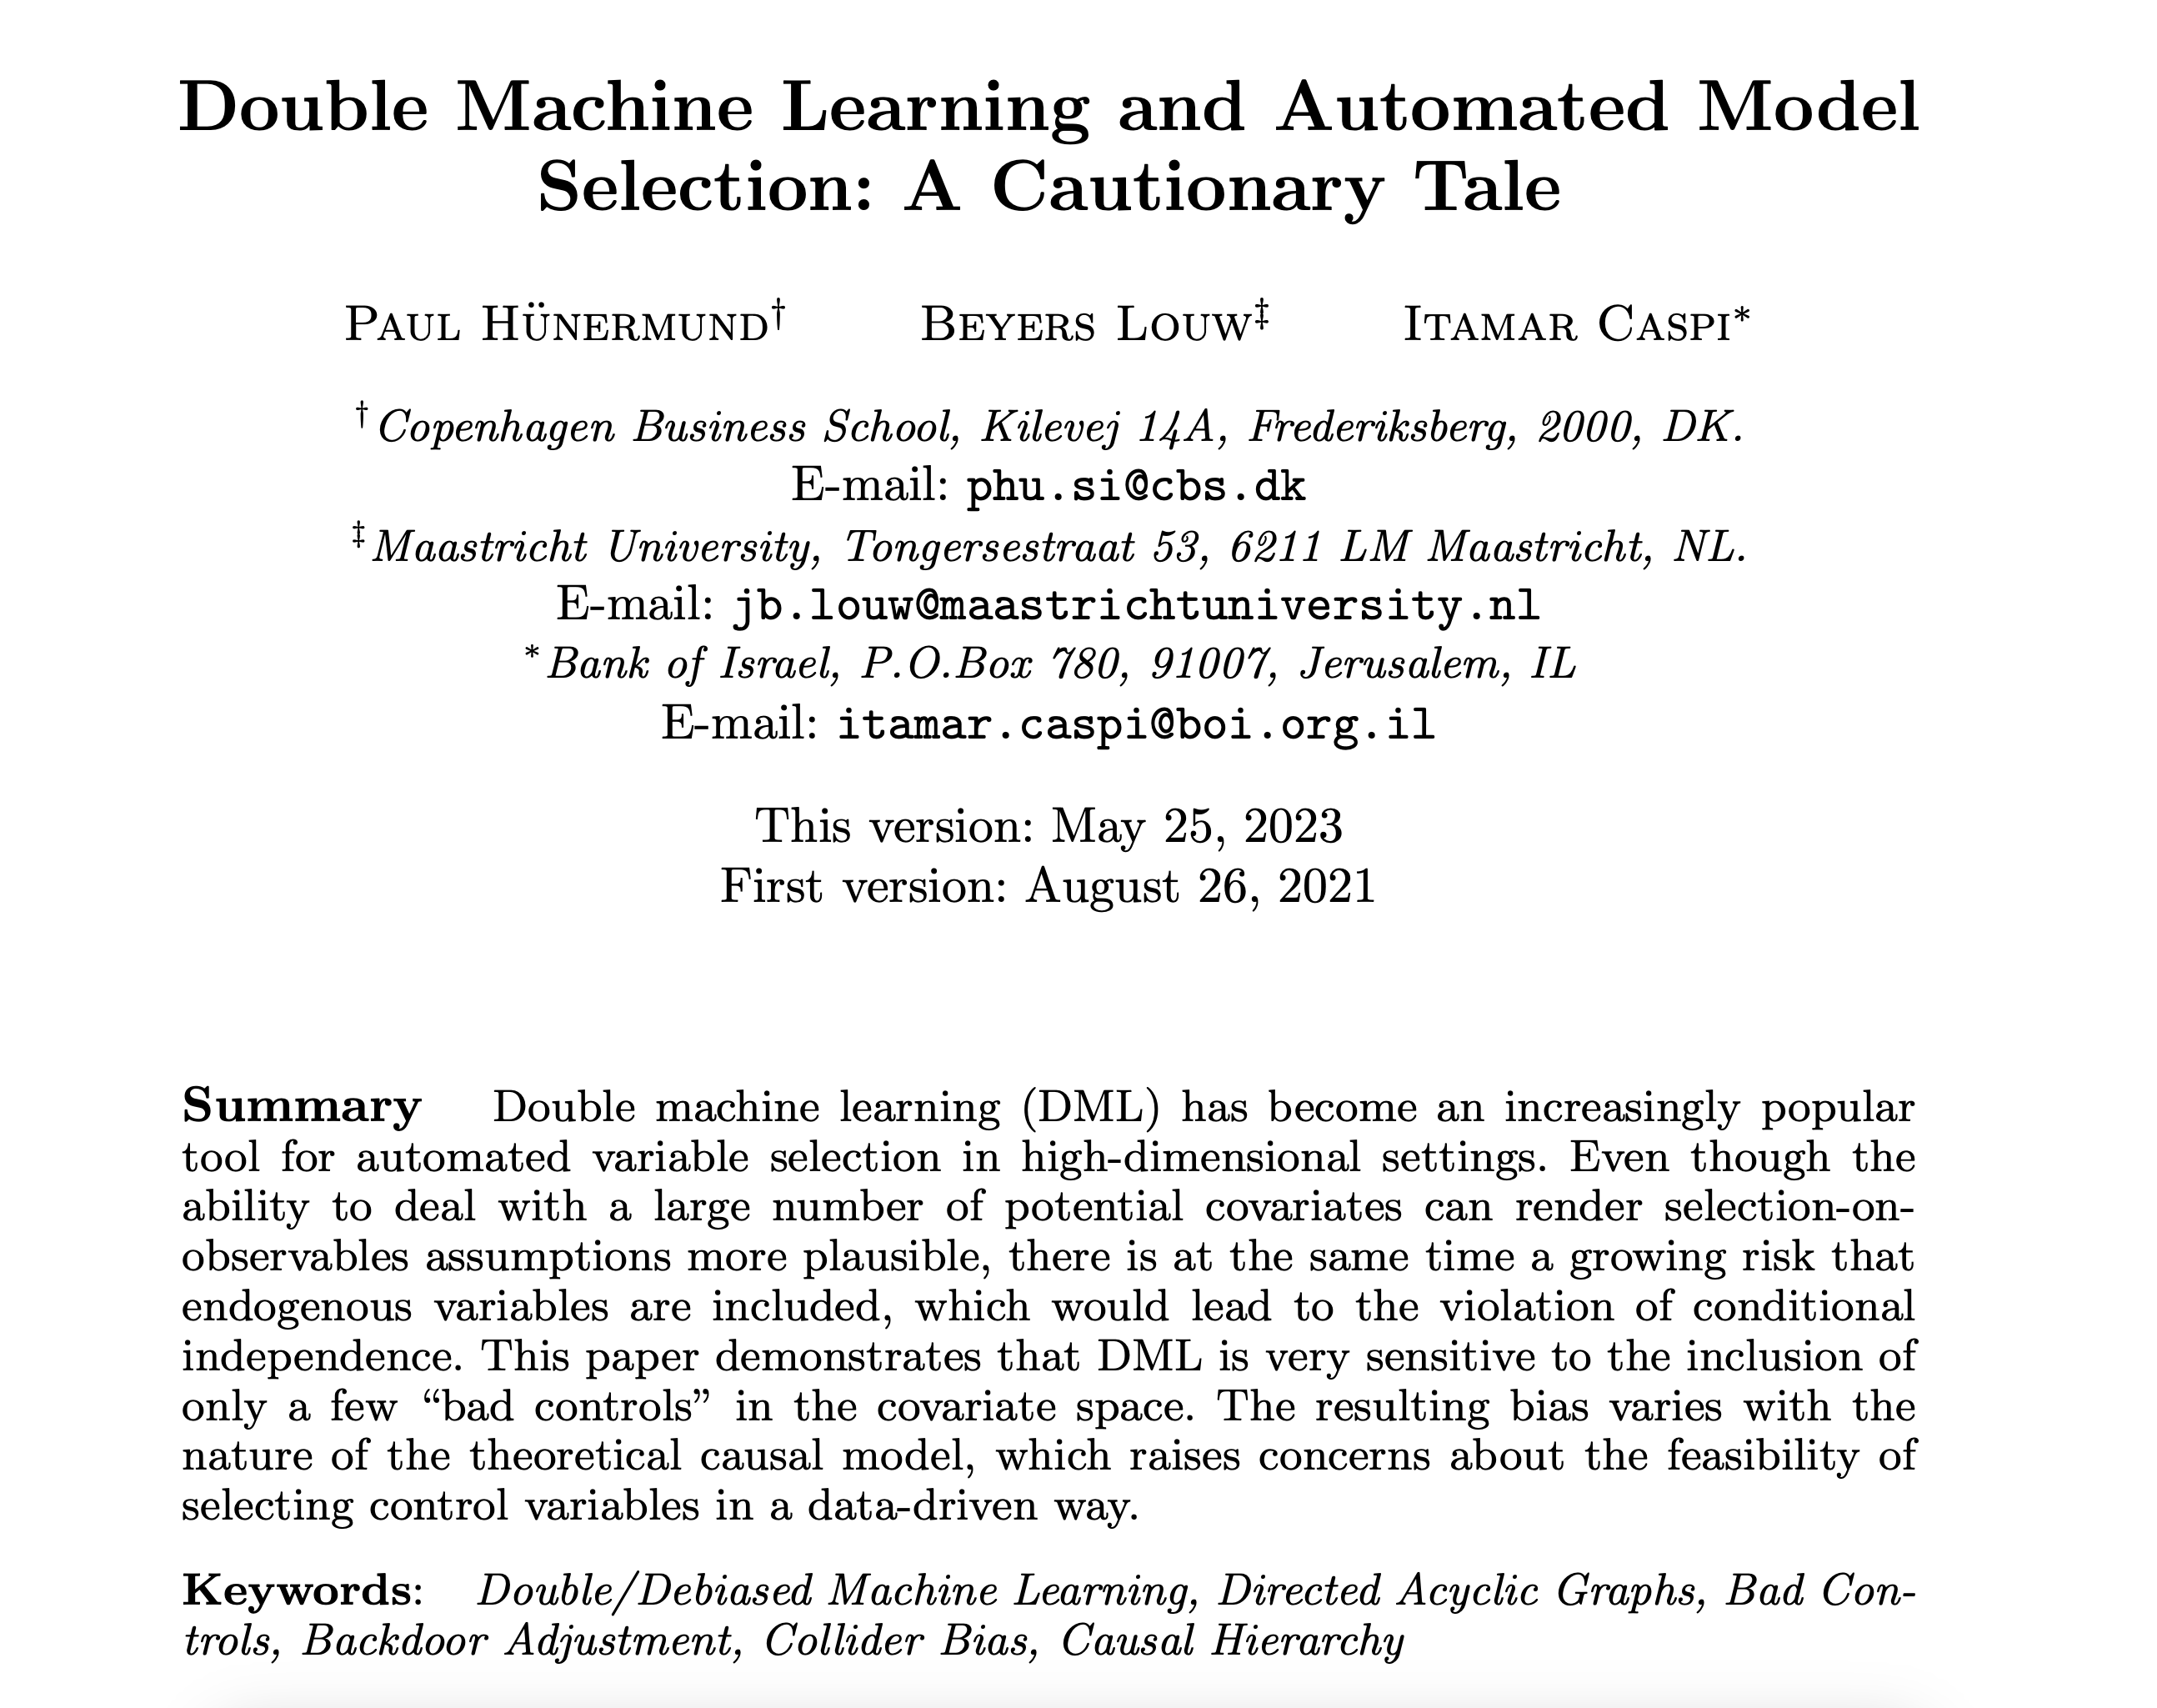
\includegraphics[scale=0.25]{./lecture_includes/paul_dml}
  \end{figure}

\end{frame}




\begin{frame}{Covariate selection without DAGs}

\begin{itemize}
\item What if you don't have a DAG you feel confident about?  
	\begin{enumerate}
	\item Include confounders that you feel pretty confident are there 
	\item Include covariates that are \emph{highly predictive} of the missing counterfactual (e.g., $Y^0$ for the ATT)
	\item Avoid outcomes (even though that still won't address M-bias colliders)
	\end{enumerate}
\item While this approach may be less formalized, you are at least reasoning about the treatment assignment mechanism as opposed to just including whatever variables you have laying around (avoid the ``kitchen sink regressions'')
\end{itemize}

\end{frame}

\begin{frame}{Falsifications as a test}

\begin{itemize}
\item Covariates should not be affected by the treatment, so examining them as falsifications can help establish the credibility of unconfoundedness
\item Imbens and Rubin (2015) suggested using the lagged outcome (pre-treatment) as a way of checking, as those have similar confounder structures
\item Falsifications too: One study questioned a finding that obesity was contagious in social networks by estimating the same model on things that cannot be contagious like acne, headaches and height and found the same things (likely confounding existed)
\end{itemize}

\end{frame}




 where the section used to sit,
% i.e. immediately before \subsection{Design Trumps Analysis}.

\section{Directed Acyclic Graphs}

\begin{frame}{Connecting today with yesterday}

\begin{itemize}
\item Day 1 we were introduced to the two defining elements of the design approach to causal inference
	\begin{enumerate}
	\item Potential Outcomes to define causal parameters (individual and average)
	\item Treatment assignment mechanism (e.g., randomization)
	\end{enumerate}
\item We also introduced the notion of ``selection bias'' and ``heterogeneous treatment effect bias''
\begin{eqnarray*}
SDO &=& ATE + \textcolor{purple}{E[Y^0|D=1]} - E[Y^0|D=0] \\
&& + (1-\pi)(ATT-ATU)
\end{eqnarray*}
\item And randomization ``deleted'' the second and third term
\end{itemize}

\end{frame}

\begin{frame}

\begin{center}
\textbf{Two design traditions}
\end{center}

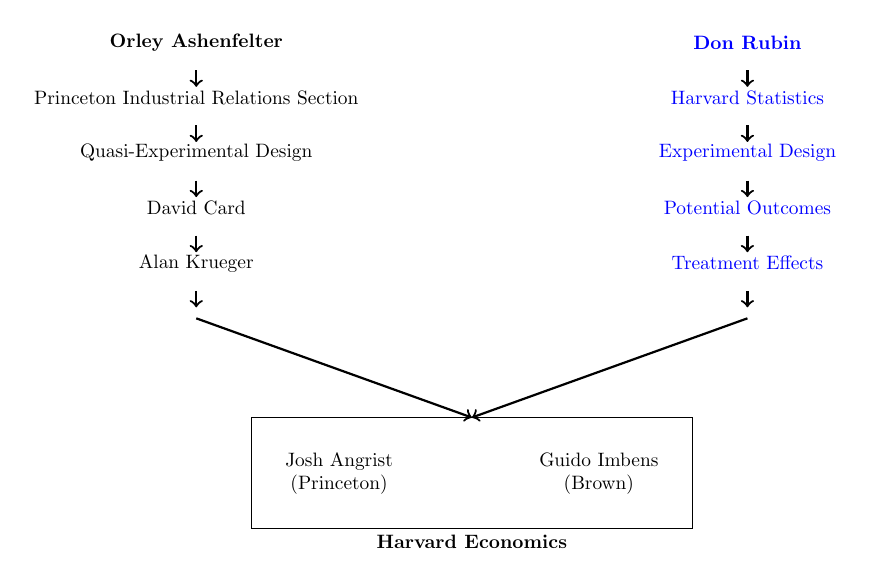
\begin{tikzpicture}[scale=0.7, every node/.style={scale=0.7}]
% Orley Ashenfelter Stream
\node at (-5,6) {\textbf{Orley Ashenfelter}};
\draw[->, thick] (-5,5.5) -- (-5,5.2);
\node at (-5,5) {Princeton Industrial Relations Section};
\draw[->, thick] (-5,4.5) -- (-5,4.2);
\node at (-5,4) {Quasi-Experimental Design};
\draw[->, thick] (-5,3.5) -- (-5,3.2);
\node at (-5,3) {David Card};
\draw[->, thick] (-5,2.5) -- (-5,2.2);
\node at (-5,2) {Alan Krueger};
\draw[->, thick] (-5,1.5) -- (-5,1.2);

% Don Rubin Stream
\begin{scope}[every node/.append style={text=blue}]
\node at (5,6) {\textbf{Don Rubin}};
\draw[->, thick] (5,5.5) -- (5,5.2);
\node at (5,5) {Harvard Statistics};
\draw[->, thick] (5,4.5) -- (5,4.2);
\node at (5,4) {Experimental Design};
\draw[->, thick] (5,3.5) -- (5,3.2);
\node at (5,3) {Potential Outcomes};
\draw[->, thick] (5,2.5) -- (5,2.2);
\node at (5,2) {Treatment Effects};
\draw[->, thick] (5,1.5) -- (5,1.2);
\end{scope}

% Arrow from Orley Ashenfelter and Don Rubin streams to bottom rectangle
\draw[->, thick] (-5,1) -- (0,-0.8);
\draw[->, thick] (5,1) -- (0,-0.8);

% Bottom Rectangle
\node[draw, minimum width=8cm, minimum height=2cm, anchor=north] at (0,-0.8) {
    \begin{tabular}{c}
        Josh Angrist \\
        (Princeton)
    \end{tabular}
    \hspace{2cm}
    \begin{tabular}{c}
        Guido Imbens \\
        (Brown)
    \end{tabular}
};
\node[anchor=north] at (0,-2.8) {\textbf{Harvard Economics}};

\end{tikzpicture}

\end{frame}

\begin{frame}{Confounding}

\begin{itemize}

\item One of the main ways that the "design" part of this branch focused on was "adjusting for observables" that could be violating independence
\item This work goes back a long way -- even to Yule in the 19th century who used regression with controls
\item But we want to now give a more modern, comprehensive review of this material
\item We will use graphs to help us better understand when we can eliminate selection bias by simply including observables controls, or what is called "unconfoundedness", "ignorability", "selection on observables" or "exogeneity"

\end{itemize}

\end{frame}



\subsection{Graph notation}

\begin{frame}{Judea Pearl, 2011 Turing Award winner}

  \begin{figure}
    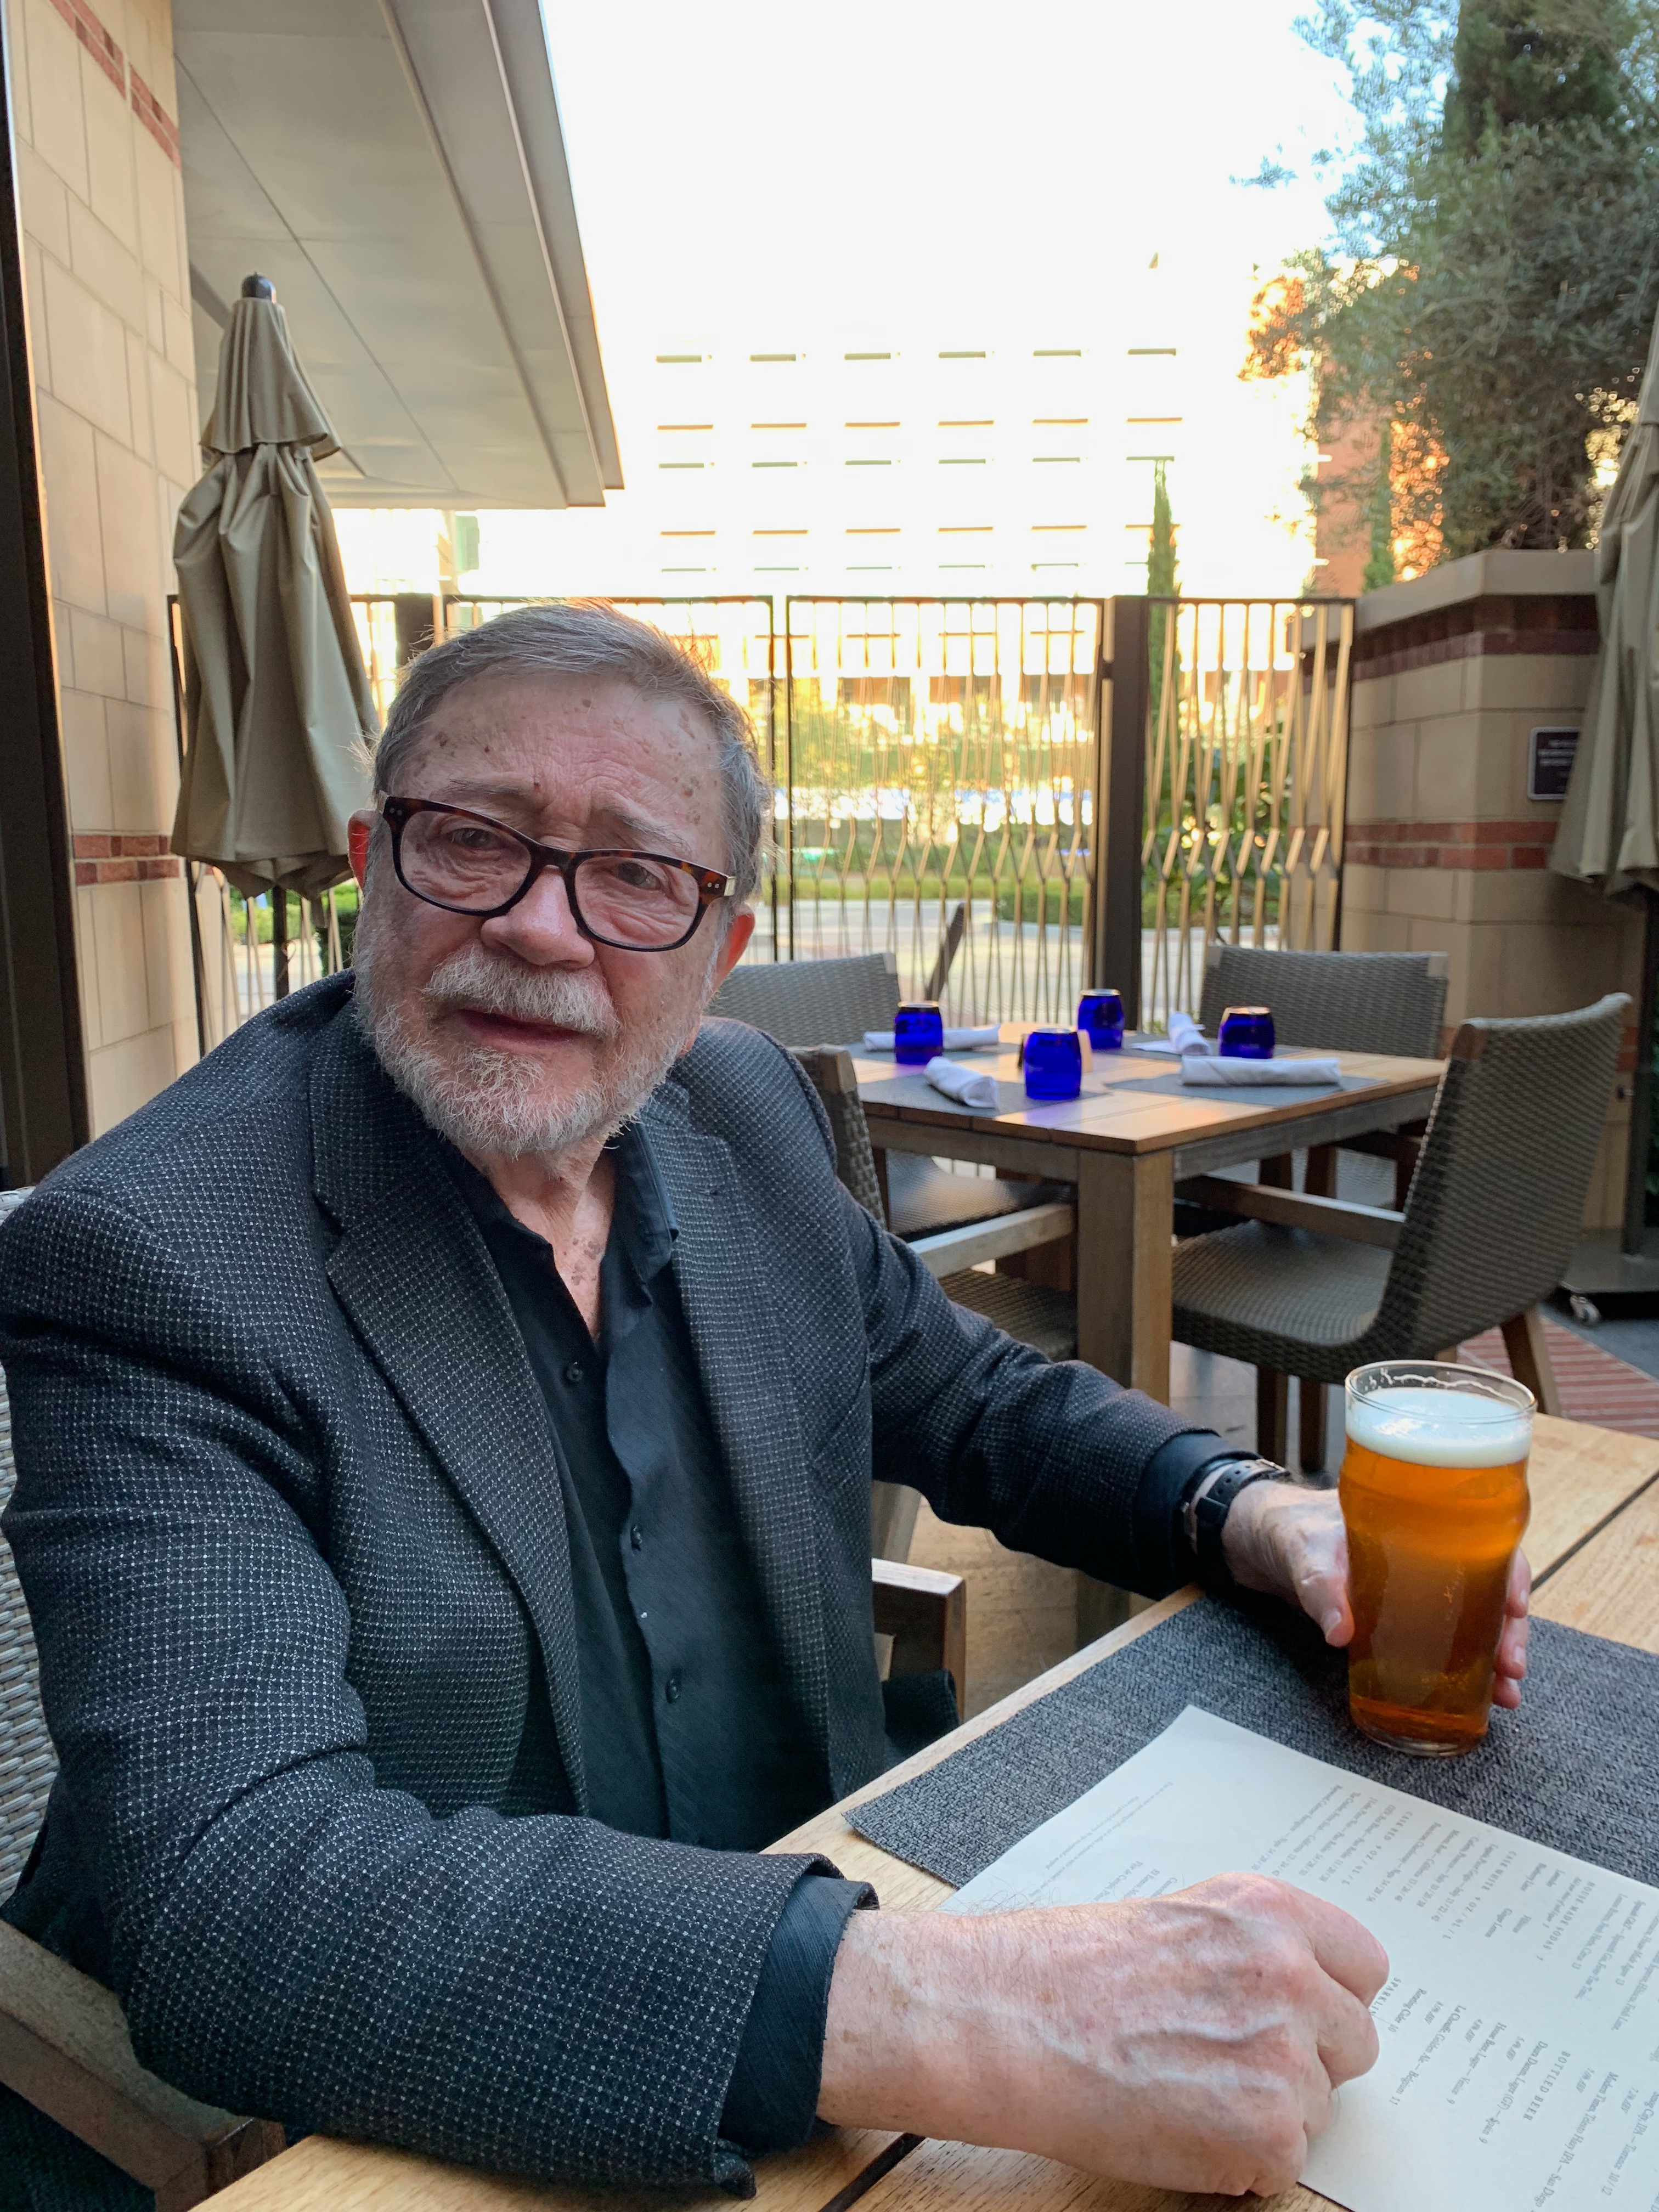
\includegraphics[scale=0.05]{./lecture_includes/pearl_ipa.jpg}
  \end{figure}

\end{frame}


\begin{frame}{Judea Pearl and DAGs}


  \begin{itemize}
    \item Judea Pearl and colleagues in Artificial Intelligence at UCLA developed directed acyclic graphs (DAGs) modeling to create a formalized causal inference methodology
    \item The letters mean this:
    	\begin{itemize}
	\item \textbf{D}: Directed.  This is a reference to graph theory.  Direct edges represent causal pathways from one variable to another
	\item \textbf{A}: Acyclic.  This means that the causal pathway only moves in one direction.  No loops or feedbacks. Limits its ability to represent many things in economics (e.g., reverse causality, simultaneous equations)
	\item \textbf{G}: Graphs. And this is also a reference to graph theory.  These are represented with a system of nodes and arrows
	\end{itemize}
    \item We'll use these to understand selection on observables ("unconfoundedness") and instrumental variables
  \end{itemize}

\end{frame}






\begin{frame}{Causal model}

  \begin{itemize}
  \item DAGs use the prior information you have about the treatment assignment and the determinants of the outcome to model the various channels (both direct and through backdoors) that the treatment causes the outcome
	\item If your knowledge of the DAG is correct, then identification of average treatment effects becomes straightforward -- but there are few ways to ``prove'' the DAG so their popularity among economists has been met with skepticism
	\item But for the selection of covariates to be used in any method that controls for covariates, they are indispensable 
    \item Consider the following diagram representing the returns to education with simplified confounders
  \end{itemize}

\end{frame}


\begin{frame}[plain]

  \begin{center}
    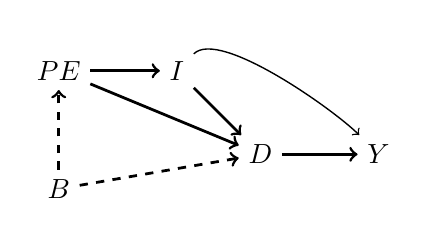
\begin{tikzpicture}[node distance=1.5cm]
      % nodes %
      \node[text centered] (d) {$D$};
      \node[right of = d, text centered] (y) {$Y$};
      \node[above left of = d, text centered] (i) {$I$};
      \node[left of = i, text centered] (pe) {$PE$};
      \node[below of = pe, text centered] (b) {$B$};
      % edges %
      \draw[->, line width= 1] (d) -- (y);
      \draw[->, line width= 1,] (i) -- (d);
      \draw[->, line width= 1,] (pe) -- (i);
      \draw[->, line width= 1,] (pe) -- (d);
      \draw[->, line width= 1, dashed] (b) -- (pe);
      \draw[->, line width= 1, dashed] (b) -- (d);
      \draw[->, line width= .5] (i) to [out=45,in=135, looseness=0.5] (y);
    \end{tikzpicture}
  \end{center}

  \bigskip
  \begin{itemize}
    \item $B$ is a \textbf{parent} of $PE$ and $D$
    \item $PE$ and $D$ are \textbf{descendants} of $B$
    \item There is a \textbf{direct (causal) path} from $D$ to $Y$
    \item There is a \textbf{mediated (causal) path} from $B$ to $Y$ through $D$
    \item There are a lot of \textbf{paths} from $PE$ to $Y$ but none are direct, and some go ``downstream'' but others go ``upstream''
  \end{itemize}
\end{frame}





\begin{frame}{Creating your DAG}

	\begin{itemize}
	\item Create a DAG that is a reasonable and honest approximation of $D$ and $Y$ parents (confounders) as well as direct and indirect effects of $D$ on $Y$
	\item Where there is uncertainty, you have to acknowledge that in the DAG, and where there are beliefs, you acknowledge that too
	\item We get ideas for DAGs from theory, models, observation, experience, prior studies, intuition, as well as conversations with domain experts
	\end{itemize}

\end{frame}


\begin{frame}{DAGs Pre-Analysis Stage}

	\begin{itemize}
	\item DAGs are meant to represent the truth about treatment assignment mechanisms and selection for the units in \emph{your data} 
	\item But creating the DAGs after you collect the data may be cheating as you're able to draw the DAG based simply on what you have rather than what is true
	\item What determines the treatment in \emph{your dataset} may be different from what determines in someone else's even if the topic is the same
	\item You'll need to spend time before your projects understanding why units in your data enrolled in the treatment -- this isn't something you do after your get the data 
	\end{itemize}
\end{frame}




% 	\item The DAG is a reasonable approximation of all common parents of $D$ and $Y$ (confounders) and direct relationships between $D and $Y$


\subsection{Backdoor criterion}


\begin{frame}{Confounding}

  \begin{itemize}
  	\item The covariates you need to control for under unconfoundedness are called \textbf{confounders}, as confounders create backdoor paths from treatment to outcome
          \item Confounders create selection bias \\

          \begin{center}
            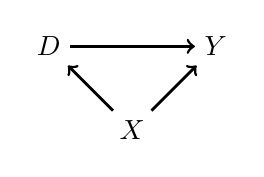
\begin{tikzpicture}
              [node distance=1.5cm]
              % nodes %
              \node[text centered] (d) {$D$};
              \node[below right of = d, text centered] (x) {$X$};
              \node[above right of = x, text centered] (y) {$Y$};

              % edges %
              \draw[->, line width= 1] (d) -- (y);
              \draw[->, line width= 1] (x) -- (d);
              \draw[->, line width= 1] (x) -- (y);
            \end{tikzpicture}
          \end{center}

          \item Our knowledge about this will enable us to select the correct covariates (but not necessarily the correct specification)
          \item Let's look at \texttt{confounders.do} in our shared labs (/Labs/DAGs)
  \end{itemize}
\end{frame}

\begin{frame}{Backdoor Paths}

  \begin{itemize}
    \item Confounding creates \textbf{backdoor paths} between treatment and outcome ($D\leftarrow X\rightarrow Y$) -- i.e., spurious correlations
		\begin{itemize}
		\item Distinct from something called a collider path ($D \rightarrow X \leftarrow Y$)
		\item Distinct from something called a mediator path ($D \rightarrow X \rightarrow Y$)
		\end{itemize}
    \item We can ``block'' any particular backdoor path by conditioning on variable $X$ so long as it is not a collider (visualized here with a square over X)

  \end{itemize}

  \begin{center}
    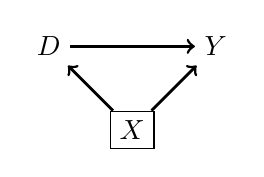
\begin{tikzpicture}
      [node distance=1.5cm]
      % nodes %
      \node[text centered] (d) {$D$};
      \node[below right of = d, text centered, rectangle, draw, thin] (x) {$X$};
      \node[above right of = x, text centered] (y) {$Y$};

      % edges %
      \draw[->, line width= 1] (d) -- (y);
      \draw[->, line width= 1] (x) -- (d);
      \draw[->, line width= 1] (x) -- (y);
    \end{tikzpicture}
  \end{center}

\end{frame}

\begin{frame}{Backdoor Paths}

  \begin{itemize}
    \item Once we condition on $X$, we can calculate average differences in $Y$ by treatment status to obtain an estimate of an aggregate causal parameter
    \item There are many methods for doing this and we cover them today -- regression, matching, stratification, weights
    \item But all of them at their fundamental level are calculating simple differences in mean outcomes for given values of $X$ and then taking weighted averages

  \end{itemize}

  \begin{center}
    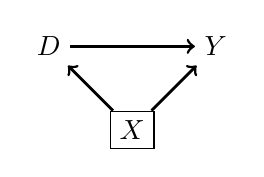
\begin{tikzpicture}
      [node distance=1.5cm]
      % nodes %
      \node[text centered] (d) {$D$};
      \node[below right of = d, text centered, rectangle, draw, thin] (x) {$X$};
      \node[above right of = x, text centered] (y) {$Y$};

      % edges %
      \draw[->, line width= 1] (d) -- (y);
      \draw[->, line width= 1] (x) -- (d);
      \draw[->, line width= 1] (x) -- (y);
    \end{tikzpicture}
  \end{center}

\end{frame}


\begin{frame}{Backdoor Paths}

  \begin{itemize}

	\item When all backdoor paths from $D$ to $Y$ are blocked, then the only remaining path between $D$ to $Y$ is the causal path
	\item We call this satisfying the backdoor criterion using Pearl's DAG terminology, and we call it unconfoundedness using Rubin's potential outcomes terminology (which I'll discuss later)

  \end{itemize}

  \begin{center}
    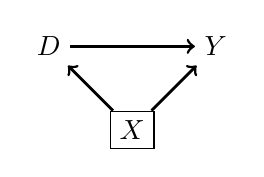
\begin{tikzpicture}
      [node distance=1.5cm]
      % nodes %
      \node[text centered] (d) {$D$};
      \node[below right of = d, text centered, rectangle, draw, thin] (x) {$X$};
      \node[above right of = x, text centered] (y) {$Y$};

      % edges %
      \draw[->, line width= 1] (d) -- (y);
      \draw[->, line width= 1] (x) -- (d);
      \draw[->, line width= 1] (x) -- (y);
    \end{tikzpicture}
  \end{center}

\end{frame}








\begin{frame}{Backdoor criterion}


  \begin{block}{Backdoor criterion}
    Conditioning on $X$ satisfies the backdoor criterion with respect to $(D,Y)$ directed path if:
    \begin{enumerate}
      \item All backdoor paths are blocked by $X$
      \item No element of $X$ is a collider

    \end{enumerate}

    
  \end{block}
       Conditioning on a non-collider is sufficient to closing a backdoor path even if it's been opened by conditioning on a collider, so just be sure to close a backdoor path if you opened it with a collider


\end{frame}

\begin{frame}{What control strategy meets the backdoor criterion?}
  \begin{itemize}
    \item List all backdoor paths from $D$ to $Y$. I'll wait.

          \begin{center}
            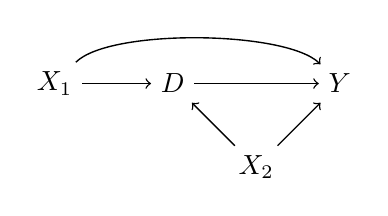
\begin{tikzpicture}
              [node distance=1.5cm]
              % nodes %
              \node[text centered,rectangle,thin] (x1) {$X_1$};
              \node[right of = x1, text centered] (d) {$D$};
              \node[below right of = d, text centered] (x2) {$X_2$};
              \node[above right of = x2, text centered] (y) {$Y$};

              % edges %
              \draw[->, line width= .5] (x1) -- (d);
              \draw[->, line width= .5] (d) -- (y);
              \draw[->, line width= .5] (x2) -- (d);
              \draw[->, line width= .5] (x2) -- (y);
              \draw[->, line width= .5] (x1) to [out=45,in=135, looseness=0.5] (y);
            \end{tikzpicture}
          \end{center}

    \item What are the necessary and sufficient set of controls which will satisfy the backdoor criterion?
  \end{itemize}

  \framebreak




\end{frame}


\begin{frame}{What if you have an unobservable?}


  \begin{itemize}
    \item List all the backdoor paths from $D$ to $Y$.

          \begin{center}
            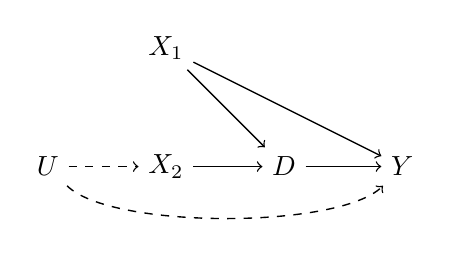
\begin{tikzpicture}
              [node distance=1.5cm]
              % nodes %
              \node[text centered] (u) {$U$};
              \node[right of = u, text centered] (x2) {$X_2$};
              \node[above of = x2, text centered] (x1) {$X_1$};
              \node[right of = x2, text centered] (d) {$D$};
              \node[right of = d, text centered] (y) {$Y$};

              % edges %
              \draw[->, line width= .5, dashed] (u) -- (x2);
              \draw[->, line width= .5] (x2) -- (d);
              \draw[->, line width= .5] (x1) -- (d);
              \draw[->, line width= .5] (x1) -- (y);
              \draw[->, line width= .5] (d) -- (y);
              \draw[->, line width= .5, dashed] (u) to [out=-45,in=-135, looseness=0.5] (y);
            \end{tikzpicture}
          \end{center}

    \item What are the necessary and sufficient set of controls which will satisfy the backdoor criterion?
    \item What about the unobserved variable, $U$?
  \end{itemize}

  \framebreak


\end{frame}

\begin{frame}{Multiple strategies}


  \begin{center}
    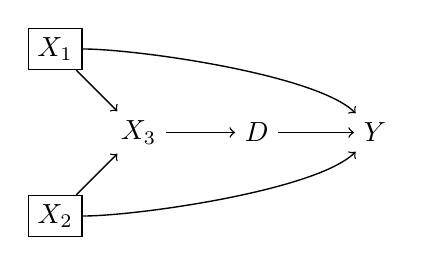
\begin{tikzpicture}
      [node distance=1.5cm, text centered]
      % nodes %
      \node[] (x3) {$X_3$};
      \node[above left of = x3,rectangle,draw,thin] (x1) {$X_1$};
      \node[below left of = x3,rectangle,draw,thin] (x2) {$X_2$};
      \node[right of = x3] (d) {$D$};
      \node[right of = d] (y) {$Y$};

      % edges %
      \draw[->, line width= .5] (x1) -- (x3);
      \draw[->, line width= .5] (x2) -- (x3);
      \draw[->, line width= .5] (x1) to [out=0,in=135, looseness=0.5] (y);
      \draw[->, line width= .5] (x2) to [out=0,in=-135, looseness=0.5] (y);
      \draw[->, line width= .5] (x3) -- (d);
      \draw[->, line width= .5] (d) -- (y);
    \end{tikzpicture}

    \vspace{1em}

    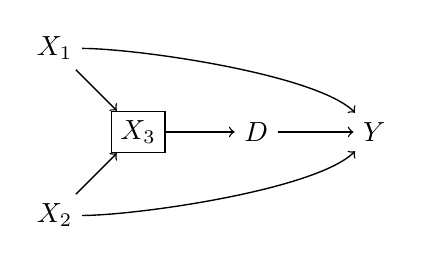
\begin{tikzpicture}
      [node distance=1.5cm, text centered]
      % nodes %
      \node[rectangle,draw,thin] (x3) {$X_3$};
      \node[above left of = x3] (x1) {$X_1$};
      \node[below left of = x3] (x2) {$X_2$};
      \node[right of = x3] (d) {$D$};
      \node[right of = d] (y) {$Y$};

      % edges %
      \draw[->, line width= .5] (x1) -- (x3);
      \draw[->, line width= .5] (x2) -- (x3);
      \draw[->, line width= .5] (x1) to [out=0,in=135, looseness=0.5] (y);
      \draw[->, line width= .5] (x2) to [out=0,in=-135, looseness=0.5] (y);
      \draw[->, line width= .5] (x3) -- (d);
      \draw[->, line width= .5] (d) -- (y);
    \end{tikzpicture}
  \end{center}

  \begin{itemize}
  \tiny
    \item Conditioning on the common causes, $X_1$ and $X_2$, is sufficient but so is conditioning on $X_3$
    \item See \texttt{confounder_multiple.do} for differences in variance -- overcontrolling is more precise
  \end{itemize}
\end{frame}






\subsection{Collider bias}

\begin{frame}{Collider bias}

\begin{itemize}
\item Backdoor paths can remain open in covariate adjustment strategies through two ways:
	\begin{enumerate}
	\item You did not close the path because you did not condition on the confounder
	\item Your conditioning variable opened up a previously closed backdoor path because on that path the variable was a \textbf{collider}
	\end{enumerate}
\item Colliders are ``bad controls'' which when you control for them, \emph{create} new previously non-existent spurious correlations (not commonly discussed, even in economics)
\item This is the risk of blindly controlling for variables -- you may inadvertently include bad or irrelevant controls
\end{itemize}

\end{frame}


\begin{frame}{Example 1: Movie stars}

  \alert{Important}: Since unconditioned colliders block back-door paths, what exactly does conditioning on a collider do? Let's illustrate with a fun example and some made-up data\\
  \begin{itemize}
    \item \underline{CNN.com} headline: Megan Fox voted worst -- but sexiest -- actress of 2009 \myurlshort{http://marquee.blogs.cnn.com/2009/12/30/megan-fox-voted-worst-but-sexiest-actress-of-2009/}{(link)}
    \item Are these two things actually negatively correlated in the world?
    \item Assume talent and beauty are independent, but each causes someone to become a movie star.  What's the correlation between talent and beauty for a sample of movie stars compared to the population as a whole (stars and non-stars)?
  \end{itemize}

\end{frame}


\begin{frame}{Movie star DAG}

Imagine casting directors pick movie stars based on talent and beauty

  \begin{center}
    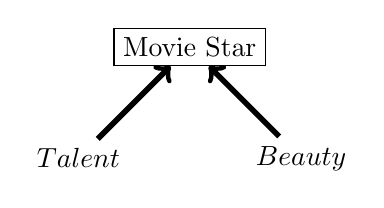
\begin{tikzpicture}
      [node distance=2cm, text centered]

      %nodes
      \node[text centered,draw,rectangle,thin] (x) {Movie Star};
      \node[below left of = x] (u1) {$Talent$};
      \node[below right of = x] (u2) {$Beauty$};

      % edges %
      \draw[->, line width= 2] (u1) -- (x);
      \draw[->, line width= 2] (u2) -- (x);
    \end{tikzpicture}
  \end{center}

Talent and beauty can become correlated even though they are independent; see \texttt{moviestar.do} or \texttt{moviestar.R}


\end{frame}

\begin{frame}[shrink=20,plain]

  \begin{figure}
    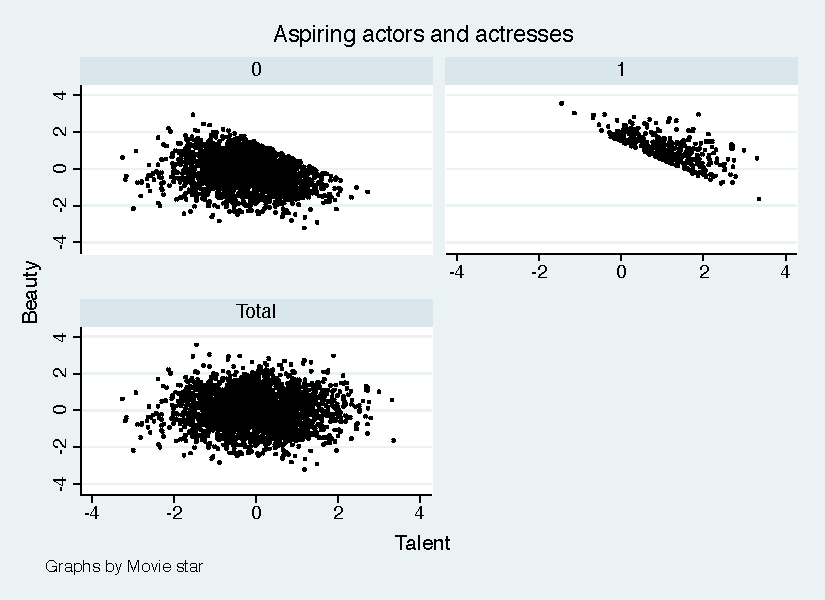
\includegraphics[height=9cm]{./lecture_includes/beauty_collider.pdf}
    \caption{Top left figure: Non-star sample scatter plot of beauty (vertical axis) and talent (horizontal axis). Top right right figure: Star sample scatter plot of beauty and talent.  Bottom left figure: Entire (stars and non-stars combined) sample scatter plot of beauty and talent.}
  \end{figure}
\end{frame}

\begin{frame}{Sample selection?}

\begin{itemize}
\item Notice that this is clear when we are focused on sample selection
\item But even a regression that included ``star'' would create the issue:$$beauty_i = \alpha + \delta talent_i + \beta star_i + \varepsilon_i$$
\item It's not just sample selection 
\end{itemize}

\end{frame}


\begin{frame}{Example 2: Discrimination}

  \begin{itemize}
    \item Let's look at another example: very common for think tanks and journalists to say that the gender gap in earnings disappears once you control for occupation.
    \item But what if occupation is a collider, which it could be in a model with occupational sorting
    \item Then controlling for occupation in a wage regression searching for discrimination can lead to all kinds of crazy results \emph{even in a simulation where we explicitly design there to be discrimination}
  \end{itemize}

\end{frame}

\begin{frame}{DAG}

  \begin{center}
    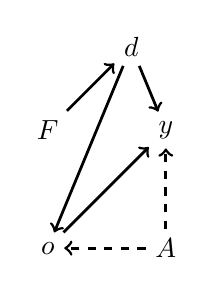
\begin{tikzpicture}
      [node distance=1.5cm]
      % nodes %
      \node[text centered] (f) {$F$};
      \node[above right of = f, text centered] (d) {$d$};
      \node[right of = f] (y) {$y$};
      \node[below  of = f, text centered] (o) {$o$};
      \node[right of = o, text centered] (a) {$A$};

      % edges %
      \draw[->, line width= 1] (f) -- (d);
      \draw[->, line width= 1] (d) -- (o);
      \draw[->, line width= 1, dashed] (a) -- (o);

      \draw[->, line width= 1] (d) -- (y);
      \draw[->, line width= 1] (o) -- (y);
      \draw[->, line width= 1, dashed] (a) -- (y);

    \end{tikzpicture}
  \end{center}

  $F$ is female, $d$ is discrimination, $o$ is occupation, $y$ is earnings and $A$ is ability. Dashed lines mean the variable cannot be observed. Note, by design, being a female has no effect on earnings or occupation, and has no relationship with ability. So earnings is coming through discrimination, occupation, and ability.

\end{frame}


\begin{frame}[plain]

  \begin{center}
    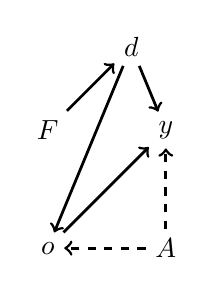
\begin{tikzpicture}
      [node distance=1.5cm]
      % nodes %
      \node[text centered] (f) {$F$};
      \node[above right of = f, text centered] (d) {$d$};
      \node[right of = f] (y) {$y$};
      \node[below  of = f, text centered] (o) {$o$};
      \node[right of = o, text centered] (a) {$A$};

      % edges %
      \draw[->, line width= 1] (f) -- (d);
      \draw[->, line width= 1] (d) -- (o);
      \draw[->, line width= 1, dashed] (a) -- (o);

      \draw[->, line width= 1] (d) -- (y);
      \draw[->, line width= 1] (o) -- (y);
      \draw[->, line width= 1, dashed] (a) -- (y);

    \end{tikzpicture}
  \end{center}


  Mediation and Backdoor paths

  \begin{enumerate}

    \item $d$ $\rightarrow o \rightarrow y$
    \item $d$ $\rightarrow o \leftarrow A \rightarrow y$
  \end{enumerate}

\end{frame}


\begin{frame}[plain, shrink=20]

  \begin{table}[htbp]\centering
    \scriptsize
    \caption{Regressions illustrating collider bias with simulated gender disparity}
    \begin{center}
      \begin{tabular}{l*{3}{c}}
        \toprule
        \multicolumn{1}{l}{Covariates: }&
        \multicolumn{1}{c}{\textbf{Unbiased combined effect}}&
        \multicolumn{1}{c}{\textbf{Biased }}&
        \multicolumn{1}{c}{\textbf{Unbiased wage effect only}}\\
        \midrule
        Female                     & -3.074*** & 0.601*** & -0.994*** \\
                                   & (0.000)   & (0.000)  & (0.000)   \\
        Occupation                 &           & 1.793*** & 0.991***  \\
                                   &           & (0.000)  & (0.000)   \\
        Ability                    &           &          & 2.017***  \\
                                   &           &          & (0.000)   \\
        \\
        \midrule
        N                          & 10,000    & 10,000   & 10,000    \\
        Mean of dependent variable & 0.45      & 0.45     & 0.45      \\
        \bottomrule
      \end{tabular}
    \end{center}
  \end{table}

  \begin{itemize}
    \item Recall we designed there to be a discrimination coefficient of -1
    \item If we do not control for occupation, then we get the combined effect of $d \rightarrow o \rightarrow y$ and $d  \rightarrow y$
    \item Because it seems intuitive to control for occupation, notice column 2 - the sign flips!
    \item We are only able to isolate the direct causal effect by conditioning on ability and occupation, but ability is unobserved
  \end{itemize}

\end{frame}

\begin{frame}[allowframebreaks,plain]

  \begin{itemize}
    \item \textbf{Colliders can be outcomes (and often those are the ones)}
          \begin{itemize}
            \item There is only one backdoor path from $D$ to $Y$

                  \begin{center}
                    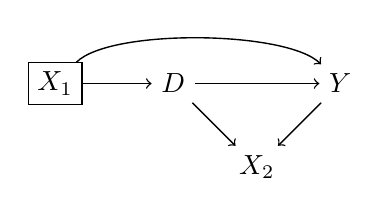
\begin{tikzpicture}
                      [node distance=1.5cm]
                      % nodes %
                      \node[text centered,draw,rectangle,thin] (x1) {$X_1$};
                      \node[right of = x1, text centered] (d) {$D$};
                      \node[below right of = d, text centered] (x2) {$X_2$};
                      \node[above right of = x2, text centered] (y) {$Y$};

                      % edges %
                      \draw[->, line width= .5] (x1) -- (d);
                      \draw[->, line width= .5] (d) -- (y);
                      \draw[->, line width= .5] (d) -- (x2);
                      \draw[->, line width= .5] (y) -- (x2);
                      \draw[->, line width= .5] (x1) to [out=45,in=135, looseness=0.5] (y);
                    \end{tikzpicture}
                  \end{center}
                  

            \item Conditioning on $X_1$ blocks the backdoor path


            \item But what if we also condition on $X_2$?

                  \begin{center}
                    \begin{tikzpicture}
                      [node distance=1.5cm]
                      % nodes %
                      \node[text centered,draw,rectangle,thin] (x1) {$X_1$};
                      \node[right of = x1, text centered] (d) {$D$};
                      \node[below right of = d, draw, rectangle, text centered] (x2) {$X_2$};
                      \node[above right of = x2, text centered] (y) {$Y$};

                      % edges %
                      \draw[->, line width= .5] (x1) -- (d);
                      \draw[->, line width= .5] (d) -- (y);
                      \draw[->, line width= .5] (d) -- (x2);
                      \draw[->, line width= .5] (y) -- (x2);
                      \draw[->, line width= .5] (x1) to [out=45,in=135, looseness=0.5] (y);
                    \end{tikzpicture}
                  \end{center}

            \item Conditioning on $X_2$ opens up a new path, creating new spurious correlations between $D$ and $Y$ 
          \end{itemize}

          \framebreak


    \item \textbf{Colliders could be pre-treatment covariates (called M-bias because it looks like an M)}
          \begin{itemize}
            \item Name the backdoor paths.  Is it open or closed?

                  \begin{center}
                    \begin{tikzpicture}
                      [node distance=1.5cm, text centered]
                      % nodes %
                      \node[] (x) {$X$};
                      \node[above left of = x] (u1) {$U_1$};
                      \node[below left of = x] (u2) {$U_2$};
                      \node[right of = x] (d) {$D$};
                      \node[right of = d] (y) {$Y$};

                      % edges %
                      \draw[->, line width= .5, dashed] (u1) -- (x);
                      \draw[->, line width= .5, dashed] (u2) -- (x);
                      \draw[->, line width= .5, dashed] (u1) to [out=0,in=135, looseness=0.5] (y);
                      \draw[->, line width= .5, dashed] (u2) to [out=0,in=-135, looseness=0.5] (d);
                      \draw[->, line width= .5] (d) -- (y);
                    \end{tikzpicture}
                  \end{center}

            \item But what if we condition on $X$?

                  \begin{center}
                    \begin{tikzpicture}
                      [node distance=1.5cm, text centered]
                      % nodes %
                      \node[text centered,draw,rectangle,thin] (x) {$X$};
                      \node[above left of = x] (u1) {$U_1$};
                      \node[below left of = x] (u2) {$U_2$};
                      \node[right of = x] (d) {$D$};
                      \node[right of = d] (y) {$Y$};

                      % edges %
                      \draw[->, line width= .5, dashed] (u1) -- (x);
                      \draw[->, line width= .5, dashed] (u2) -- (x);
                      \draw[->, line width= .5, dashed] (u1) to [out=0,in=135, looseness=0.5] (y);
                      \draw[->, line width= .5, dashed] (u2) to [out=0,in=-135, looseness=0.5] (d);
                      \draw[->, line width= .5] (d) -- (y);
                    \end{tikzpicture}
                  \end{center}


          \end{itemize}
  \end{itemize}
  \framebreak


\end{frame}


\begin{frame}{M-bias as collider}

  \centering
  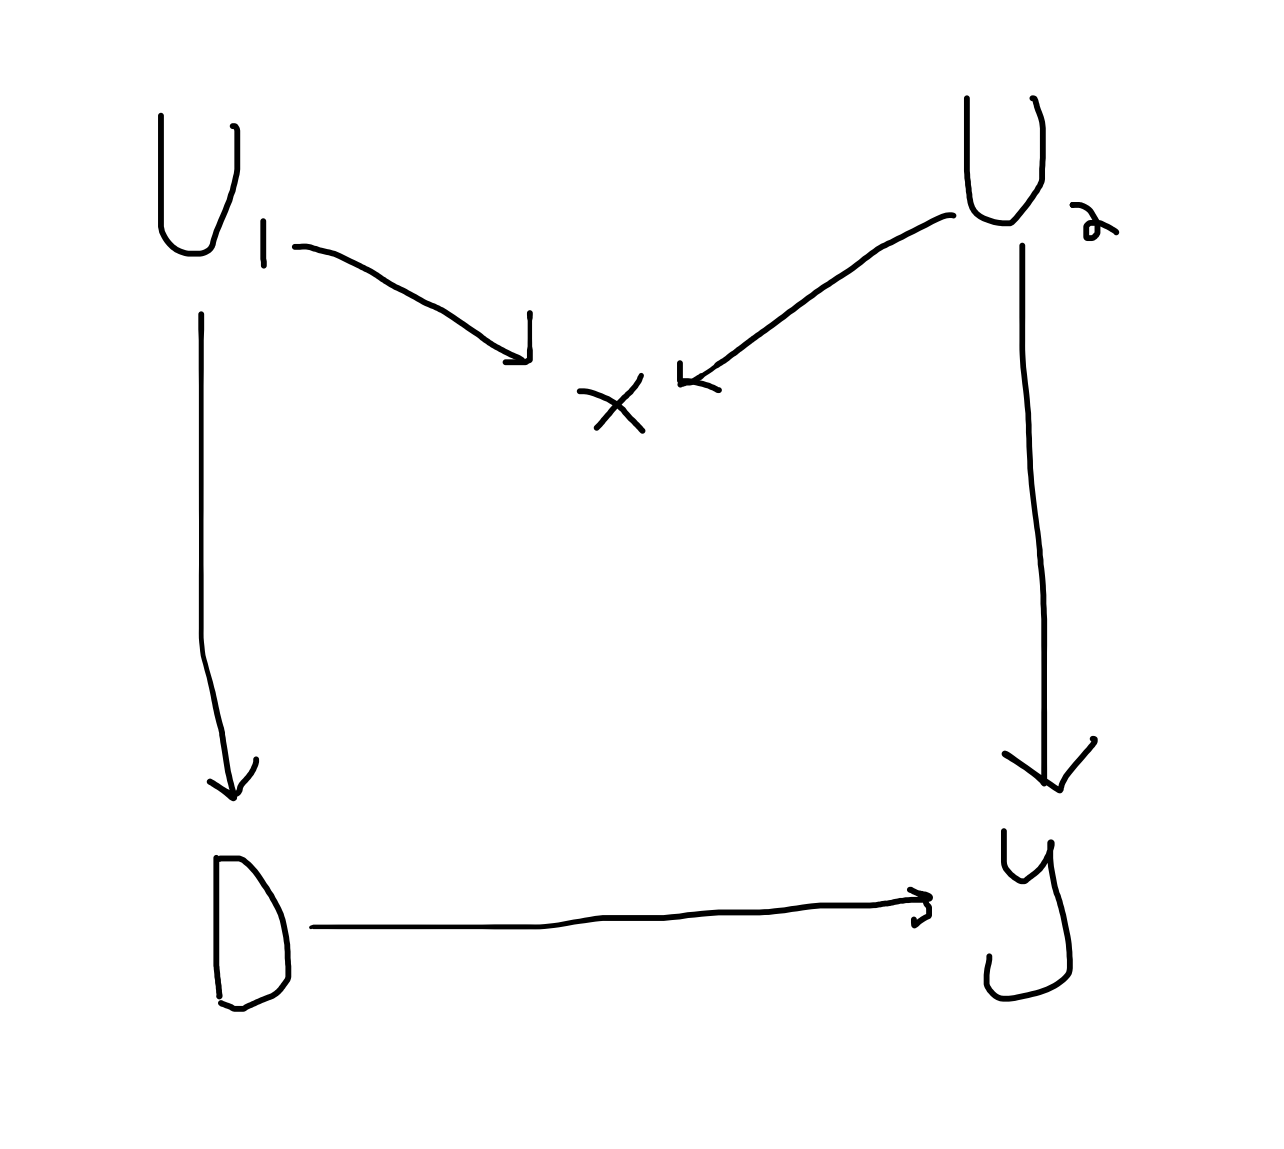
\includegraphics[height=5.8cm, width=10cm]{./lecture_includes/mbias}

\footnotesize
$X$ is pre-treatment, but if you conditioned on it, then $D\leftarrow U1 \rightarrow \mbox{X} \leftarrow U2 \rightarrow Y$ and $X$ is a collider. Colliders take strange forms, so the conditioning set \emph{must} be thoughtfully chosen based on being a strong predictor of $Y^0$, preferably based on expert knowledge and not a kitchen sink of all available regressors

\end{frame}


\begin{frame}{Testing the Validity of the DAG}

  \begin{itemize}
    \item The DAG makes testable predictions
    \item Conditional on $D$ and $I$, parental education ($PE$) should no longer be correlated with $Y$
    \item Can be hard to figure this out by hand, but software can help (e.g., Daggity.net is browser based, Causal Fusion is more advanced)
    \item Causal algorithms tend to be DAG based and are becoming popular in industry 
  \end{itemize}

  \begin{center}
    \begin{tikzpicture}[node distance=1.5cm]
      % nodes %
      \node[text centered] (d) {$D$};
      \node[right of = d, text centered] (y) {$Y$};
      \node[above left of = d, text centered] (i) {$I$};
      \node[left of = i, text centered] (pe) {$PE$};
      \node[below of = pe, text centered] (b) {$B$};
      % edges %
      \draw[->, line width= 1] (d) -- (y);
      \draw[->, line width= 1,] (i) -- (d);
      \draw[->, line width= 1,] (pe) -- (i);
      \draw[->, line width= 1,] (pe) -- (d);
      \draw[->, line width= 1, dashed] (b) -- (pe);
      \draw[->, line width= 1, dashed] (b) -- (d);
      \draw[->, line width= .5] (i) to [out=45,in=135, looseness=0.5] (y);
    \end{tikzpicture}
  \end{center}

\end{frame}




\begin{frame}{Contrast this with ordinary practices}

\begin{itemize}
\item Person attempts to ``control for omitted variable bias'' by including as many ``controls'' as possible
\item Person does not even attempt to think about treatment assignment mechanism and therefore has no idea what variables are colliders, covariates or confounders
\item Machine learning can be ``naive'' too if the large dimension of features includes unknowingly colliders
\end{itemize}

\end{frame}

\begin{frame}{}

  \begin{figure}
    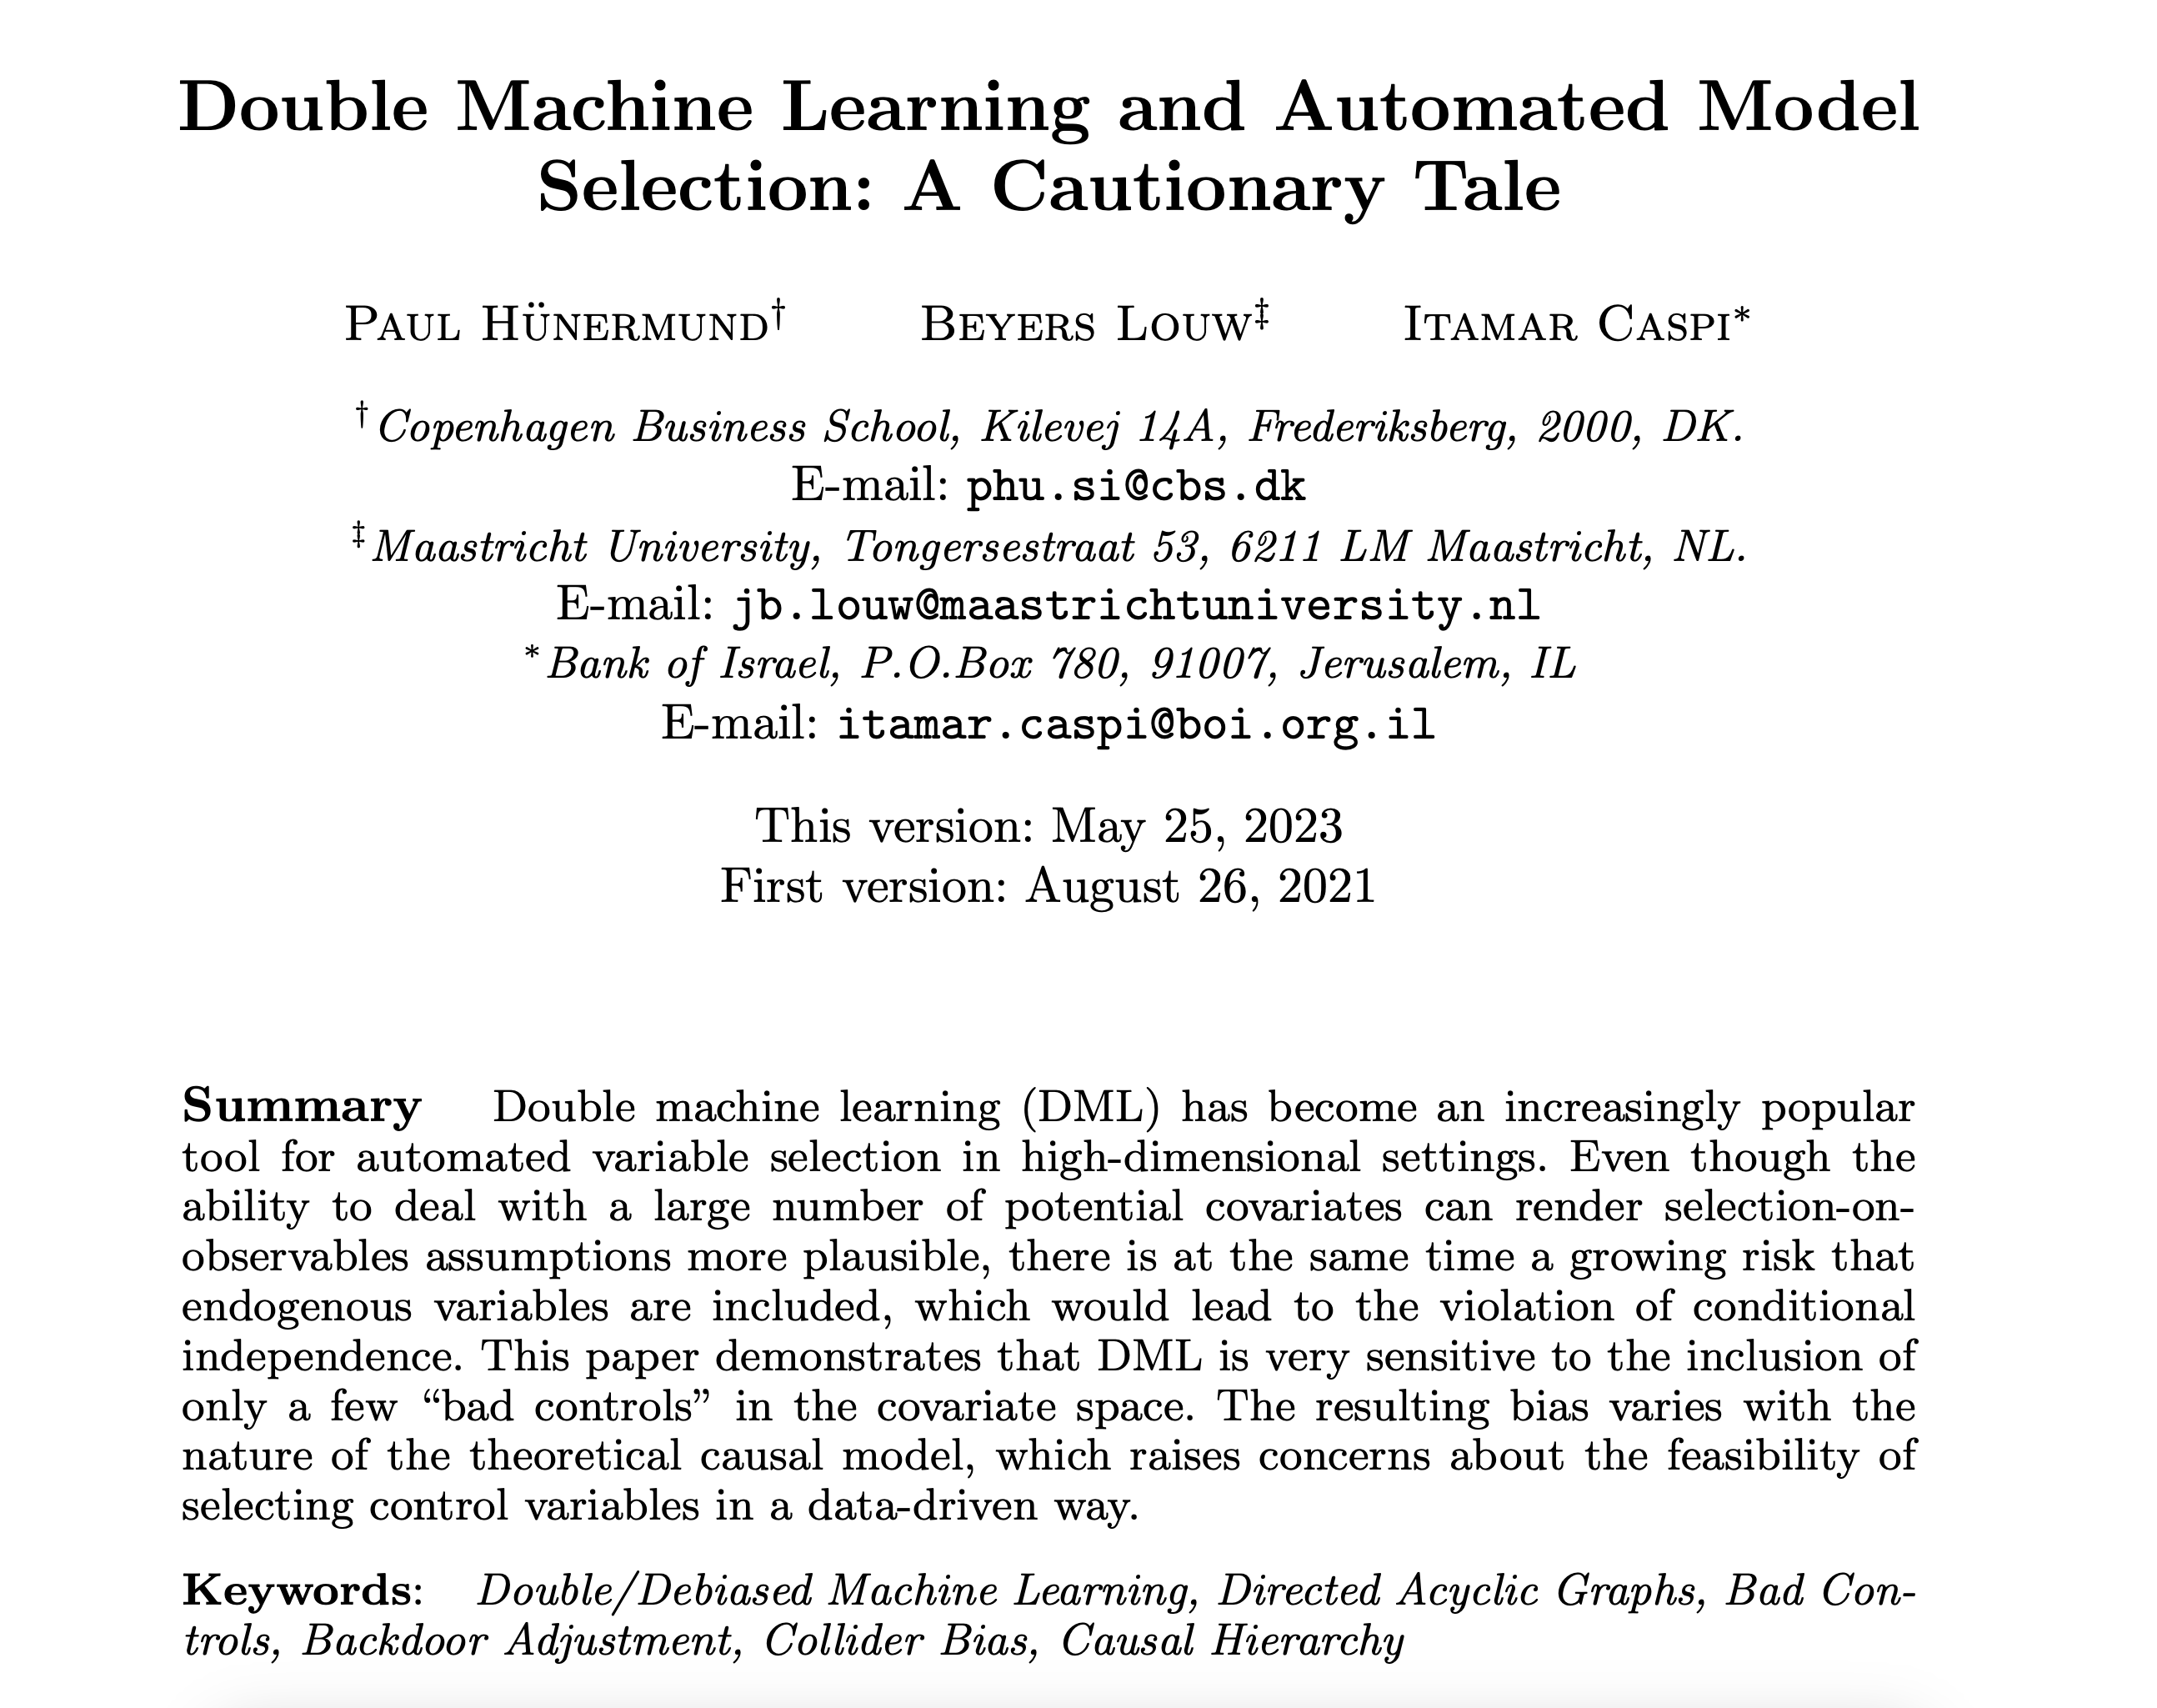
\includegraphics[scale=0.25]{./lecture_includes/paul_dml}
  \end{figure}

\end{frame}




\begin{frame}{Covariate selection without DAGs}

\begin{itemize}
\item What if you don't have a DAG you feel confident about?  
	\begin{enumerate}
	\item Include confounders that you feel pretty confident are there 
	\item Include covariates that are \emph{highly predictive} of the missing counterfactual (e.g., $Y^0$ for the ATT)
	\item Avoid outcomes (even though that still won't address M-bias colliders)
	\end{enumerate}
\item While this approach may be less formalized, you are at least reasoning about the treatment assignment mechanism as opposed to just including whatever variables you have laying around (avoid the ``kitchen sink regressions'')
\end{itemize}

\end{frame}

\begin{frame}{Falsifications as a test}

\begin{itemize}
\item Covariates should not be affected by the treatment, so examining them as falsifications can help establish the credibility of unconfoundedness
\item Imbens and Rubin (2015) suggested using the lagged outcome (pre-treatment) as a way of checking, as those have similar confounder structures
\item Falsifications too: One study questioned a finding that obesity was contagious in social networks by estimating the same model on things that cannot be contagious like acne, headaches and height and found the same things (likely confounding existed)
\end{itemize}

\end{frame}




 where the section used to sit,
% i.e. immediately before \subsection{Design Trumps Analysis}.

\section{Directed Acyclic Graphs}

\begin{frame}{Connecting today with yesterday}

\begin{itemize}
\item Day 1 we were introduced to the two defining elements of the design approach to causal inference
	\begin{enumerate}
	\item Potential Outcomes to define causal parameters (individual and average)
	\item Treatment assignment mechanism (e.g., randomization)
	\end{enumerate}
\item We also introduced the notion of ``selection bias'' and ``heterogeneous treatment effect bias''
\begin{eqnarray*}
SDO &=& ATE + \textcolor{purple}{E[Y^0|D=1]} - E[Y^0|D=0] \\
&& + (1-\pi)(ATT-ATU)
\end{eqnarray*}
\item And randomization ``deleted'' the second and third term
\end{itemize}

\end{frame}

\begin{frame}

\begin{center}
\textbf{Two design traditions}
\end{center}

\begin{tikzpicture}[scale=0.7, every node/.style={scale=0.7}]
% Orley Ashenfelter Stream
\node at (-5,6) {\textbf{Orley Ashenfelter}};
\draw[->, thick] (-5,5.5) -- (-5,5.2);
\node at (-5,5) {Princeton Industrial Relations Section};
\draw[->, thick] (-5,4.5) -- (-5,4.2);
\node at (-5,4) {Quasi-Experimental Design};
\draw[->, thick] (-5,3.5) -- (-5,3.2);
\node at (-5,3) {David Card};
\draw[->, thick] (-5,2.5) -- (-5,2.2);
\node at (-5,2) {Alan Krueger};
\draw[->, thick] (-5,1.5) -- (-5,1.2);

% Don Rubin Stream
\begin{scope}[every node/.append style={text=blue}]
\node at (5,6) {\textbf{Don Rubin}};
\draw[->, thick] (5,5.5) -- (5,5.2);
\node at (5,5) {Harvard Statistics};
\draw[->, thick] (5,4.5) -- (5,4.2);
\node at (5,4) {Experimental Design};
\draw[->, thick] (5,3.5) -- (5,3.2);
\node at (5,3) {Potential Outcomes};
\draw[->, thick] (5,2.5) -- (5,2.2);
\node at (5,2) {Treatment Effects};
\draw[->, thick] (5,1.5) -- (5,1.2);
\end{scope}

% Arrow from Orley Ashenfelter and Don Rubin streams to bottom rectangle
\draw[->, thick] (-5,1) -- (0,-0.8);
\draw[->, thick] (5,1) -- (0,-0.8);

% Bottom Rectangle
\node[draw, minimum width=8cm, minimum height=2cm, anchor=north] at (0,-0.8) {
    \begin{tabular}{c}
        Josh Angrist \\
        (Princeton)
    \end{tabular}
    \hspace{2cm}
    \begin{tabular}{c}
        Guido Imbens \\
        (Brown)
    \end{tabular}
};
\node[anchor=north] at (0,-2.8) {\textbf{Harvard Economics}};

\end{tikzpicture}

\end{frame}

\begin{frame}{Confounding}

\begin{itemize}

\item One of the main ways that the "design" part of this branch focused on was "adjusting for observables" that could be violating independence
\item This work goes back a long way -- even to Yule in the 19th century who used regression with controls
\item But we want to now give a more modern, comprehensive review of this material
\item We will use graphs to help us better understand when we can eliminate selection bias by simply including observables controls, or what is called "unconfoundedness", "ignorability", "selection on observables" or "exogeneity"

\end{itemize}

\end{frame}



\subsection{Graph notation}

\begin{frame}{Judea Pearl, 2011 Turing Award winner}

  \begin{figure}
    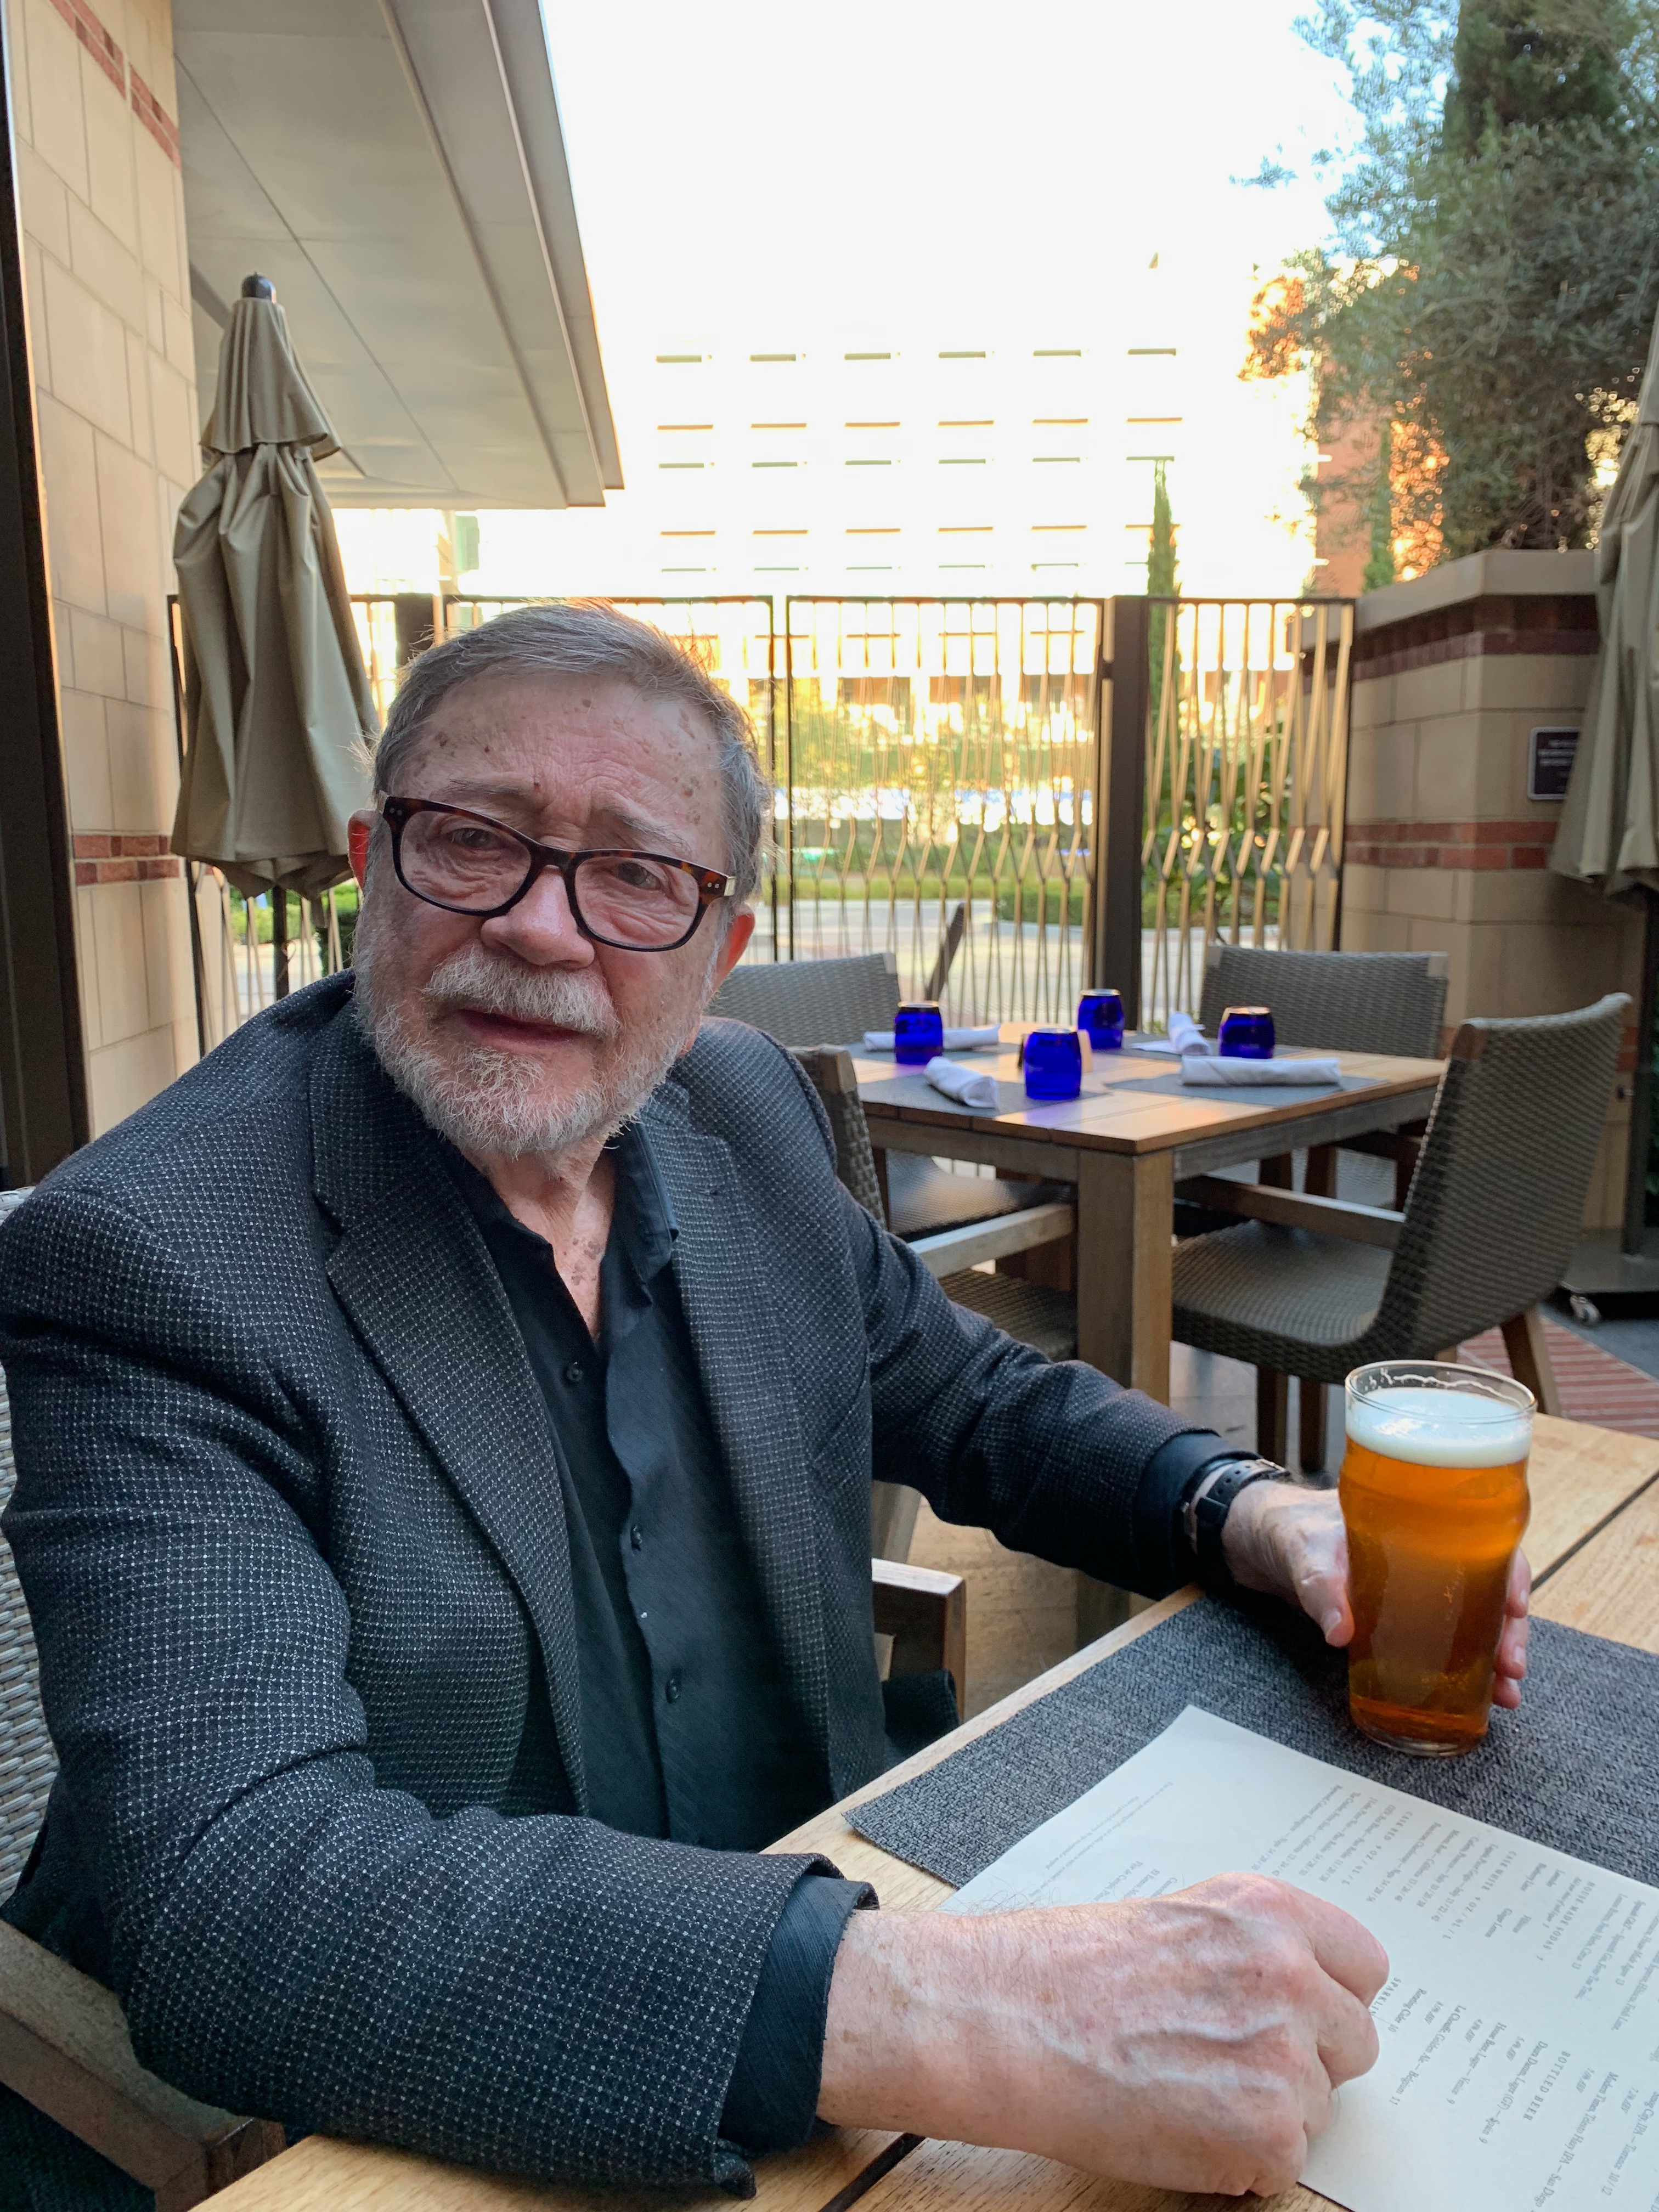
\includegraphics[scale=0.05]{./lecture_includes/pearl_ipa.jpg}
  \end{figure}

\end{frame}


\begin{frame}{Judea Pearl and DAGs}


  \begin{itemize}
    \item Judea Pearl and colleagues in Artificial Intelligence at UCLA developed directed acyclic graphs (DAGs) modeling to create a formalized causal inference methodology
    \item The letters mean this:
    	\begin{itemize}
	\item \textbf{D}: Directed.  This is a reference to graph theory.  Direct edges represent causal pathways from one variable to another
	\item \textbf{A}: Acyclic.  This means that the causal pathway only moves in one direction.  No loops or feedbacks. Limits its ability to represent many things in economics (e.g., reverse causality, simultaneous equations)
	\item \textbf{G}: Graphs. And this is also a reference to graph theory.  These are represented with a system of nodes and arrows
	\end{itemize}
    \item We'll use these to understand selection on observables ("unconfoundedness") and instrumental variables
  \end{itemize}

\end{frame}






\begin{frame}{Causal model}

  \begin{itemize}
  \item DAGs use the prior information you have about the treatment assignment and the determinants of the outcome to model the various channels (both direct and through backdoors) that the treatment causes the outcome
	\item If your knowledge of the DAG is correct, then identification of average treatment effects becomes straightforward -- but there are few ways to ``prove'' the DAG so their popularity among economists has been met with skepticism
	\item But for the selection of covariates to be used in any method that controls for covariates, they are indispensable 
    \item Consider the following diagram representing the returns to education with simplified confounders
  \end{itemize}

\end{frame}


\begin{frame}[plain]

  \begin{center}
    \begin{tikzpicture}[node distance=1.5cm]
      % nodes %
      \node[text centered] (d) {$D$};
      \node[right of = d, text centered] (y) {$Y$};
      \node[above left of = d, text centered] (i) {$I$};
      \node[left of = i, text centered] (pe) {$PE$};
      \node[below of = pe, text centered] (b) {$B$};
      % edges %
      \draw[->, line width= 1] (d) -- (y);
      \draw[->, line width= 1,] (i) -- (d);
      \draw[->, line width= 1,] (pe) -- (i);
      \draw[->, line width= 1,] (pe) -- (d);
      \draw[->, line width= 1, dashed] (b) -- (pe);
      \draw[->, line width= 1, dashed] (b) -- (d);
      \draw[->, line width= .5] (i) to [out=45,in=135, looseness=0.5] (y);
    \end{tikzpicture}
  \end{center}

  \bigskip
  \begin{itemize}
    \item $B$ is a \textbf{parent} of $PE$ and $D$
    \item $PE$ and $D$ are \textbf{descendants} of $B$
    \item There is a \textbf{direct (causal) path} from $D$ to $Y$
    \item There is a \textbf{mediated (causal) path} from $B$ to $Y$ through $D$
    \item There are a lot of \textbf{paths} from $PE$ to $Y$ but none are direct, and some go ``downstream'' but others go ``upstream''
  \end{itemize}
\end{frame}





\begin{frame}{Creating your DAG}

	\begin{itemize}
	\item Create a DAG that is a reasonable and honest approximation of $D$ and $Y$ parents (confounders) as well as direct and indirect effects of $D$ on $Y$
	\item Where there is uncertainty, you have to acknowledge that in the DAG, and where there are beliefs, you acknowledge that too
	\item We get ideas for DAGs from theory, models, observation, experience, prior studies, intuition, as well as conversations with domain experts
	\end{itemize}

\end{frame}


\begin{frame}{DAGs Pre-Analysis Stage}

	\begin{itemize}
	\item DAGs are meant to represent the truth about treatment assignment mechanisms and selection for the units in \emph{your data} 
	\item But creating the DAGs after you collect the data may be cheating as you're able to draw the DAG based simply on what you have rather than what is true
	\item What determines the treatment in \emph{your dataset} may be different from what determines in someone else's even if the topic is the same
	\item You'll need to spend time before your projects understanding why units in your data enrolled in the treatment -- this isn't something you do after your get the data 
	\end{itemize}
\end{frame}




% 	\item The DAG is a reasonable approximation of all common parents of $D$ and $Y$ (confounders) and direct relationships between $D and $Y$


\subsection{Backdoor criterion}


\begin{frame}{Confounding}

  \begin{itemize}
  	\item The covariates you need to control for under unconfoundedness are called \textbf{confounders}, as confounders create backdoor paths from treatment to outcome
          \item Confounders create selection bias \\

          \begin{center}
            \begin{tikzpicture}
              [node distance=1.5cm]
              % nodes %
              \node[text centered] (d) {$D$};
              \node[below right of = d, text centered] (x) {$X$};
              \node[above right of = x, text centered] (y) {$Y$};

              % edges %
              \draw[->, line width= 1] (d) -- (y);
              \draw[->, line width= 1] (x) -- (d);
              \draw[->, line width= 1] (x) -- (y);
            \end{tikzpicture}
          \end{center}

          \item Our knowledge about this will enable us to select the correct covariates (but not necessarily the correct specification)
          \item Let's look at \texttt{confounders.do} in our shared labs (/Labs/DAGs)
  \end{itemize}
\end{frame}

\begin{frame}{Backdoor Paths}

  \begin{itemize}
    \item Confounding creates \textbf{backdoor paths} between treatment and outcome ($D\leftarrow X\rightarrow Y$) -- i.e., spurious correlations
		\begin{itemize}
		\item Distinct from something called a collider path ($D \rightarrow X \leftarrow Y$)
		\item Distinct from something called a mediator path ($D \rightarrow X \rightarrow Y$)
		\end{itemize}
    \item We can ``block'' any particular backdoor path by conditioning on variable $X$ so long as it is not a collider (visualized here with a square over X)

  \end{itemize}

  \begin{center}
    \begin{tikzpicture}
      [node distance=1.5cm]
      % nodes %
      \node[text centered] (d) {$D$};
      \node[below right of = d, text centered, rectangle, draw, thin] (x) {$X$};
      \node[above right of = x, text centered] (y) {$Y$};

      % edges %
      \draw[->, line width= 1] (d) -- (y);
      \draw[->, line width= 1] (x) -- (d);
      \draw[->, line width= 1] (x) -- (y);
    \end{tikzpicture}
  \end{center}

\end{frame}

\begin{frame}{Backdoor Paths}

  \begin{itemize}
    \item Once we condition on $X$, we can calculate average differences in $Y$ by treatment status to obtain an estimate of an aggregate causal parameter
    \item There are many methods for doing this and we cover them today -- regression, matching, stratification, weights
    \item But all of them at their fundamental level are calculating simple differences in mean outcomes for given values of $X$ and then taking weighted averages

  \end{itemize}

  \begin{center}
    \begin{tikzpicture}
      [node distance=1.5cm]
      % nodes %
      \node[text centered] (d) {$D$};
      \node[below right of = d, text centered, rectangle, draw, thin] (x) {$X$};
      \node[above right of = x, text centered] (y) {$Y$};

      % edges %
      \draw[->, line width= 1] (d) -- (y);
      \draw[->, line width= 1] (x) -- (d);
      \draw[->, line width= 1] (x) -- (y);
    \end{tikzpicture}
  \end{center}

\end{frame}


\begin{frame}{Backdoor Paths}

  \begin{itemize}

	\item When all backdoor paths from $D$ to $Y$ are blocked, then the only remaining path between $D$ to $Y$ is the causal path
	\item We call this satisfying the backdoor criterion using Pearl's DAG terminology, and we call it unconfoundedness using Rubin's potential outcomes terminology (which I'll discuss later)

  \end{itemize}

  \begin{center}
    \begin{tikzpicture}
      [node distance=1.5cm]
      % nodes %
      \node[text centered] (d) {$D$};
      \node[below right of = d, text centered, rectangle, draw, thin] (x) {$X$};
      \node[above right of = x, text centered] (y) {$Y$};

      % edges %
      \draw[->, line width= 1] (d) -- (y);
      \draw[->, line width= 1] (x) -- (d);
      \draw[->, line width= 1] (x) -- (y);
    \end{tikzpicture}
  \end{center}

\end{frame}








\begin{frame}{Backdoor criterion}


  \begin{block}{Backdoor criterion}
    Conditioning on $X$ satisfies the backdoor criterion with respect to $(D,Y)$ directed path if:
    \begin{enumerate}
      \item All backdoor paths are blocked by $X$
      \item No element of $X$ is a collider

    \end{enumerate}

    
  \end{block}
       Conditioning on a non-collider is sufficient to closing a backdoor path even if it's been opened by conditioning on a collider, so just be sure to close a backdoor path if you opened it with a collider


\end{frame}

\begin{frame}{What control strategy meets the backdoor criterion?}
  \begin{itemize}
    \item List all backdoor paths from $D$ to $Y$. I'll wait.

          \begin{center}
            \begin{tikzpicture}
              [node distance=1.5cm]
              % nodes %
              \node[text centered,rectangle,thin] (x1) {$X_1$};
              \node[right of = x1, text centered] (d) {$D$};
              \node[below right of = d, text centered] (x2) {$X_2$};
              \node[above right of = x2, text centered] (y) {$Y$};

              % edges %
              \draw[->, line width= .5] (x1) -- (d);
              \draw[->, line width= .5] (d) -- (y);
              \draw[->, line width= .5] (x2) -- (d);
              \draw[->, line width= .5] (x2) -- (y);
              \draw[->, line width= .5] (x1) to [out=45,in=135, looseness=0.5] (y);
            \end{tikzpicture}
          \end{center}

    \item What are the necessary and sufficient set of controls which will satisfy the backdoor criterion?
  \end{itemize}

  \framebreak




\end{frame}


\begin{frame}{What if you have an unobservable?}


  \begin{itemize}
    \item List all the backdoor paths from $D$ to $Y$.

          \begin{center}
            \begin{tikzpicture}
              [node distance=1.5cm]
              % nodes %
              \node[text centered] (u) {$U$};
              \node[right of = u, text centered] (x2) {$X_2$};
              \node[above of = x2, text centered] (x1) {$X_1$};
              \node[right of = x2, text centered] (d) {$D$};
              \node[right of = d, text centered] (y) {$Y$};

              % edges %
              \draw[->, line width= .5, dashed] (u) -- (x2);
              \draw[->, line width= .5] (x2) -- (d);
              \draw[->, line width= .5] (x1) -- (d);
              \draw[->, line width= .5] (x1) -- (y);
              \draw[->, line width= .5] (d) -- (y);
              \draw[->, line width= .5, dashed] (u) to [out=-45,in=-135, looseness=0.5] (y);
            \end{tikzpicture}
          \end{center}

    \item What are the necessary and sufficient set of controls which will satisfy the backdoor criterion?
    \item What about the unobserved variable, $U$?
  \end{itemize}

  \framebreak


\end{frame}

\begin{frame}{Multiple strategies}


  \begin{center}
    \begin{tikzpicture}
      [node distance=1.5cm, text centered]
      % nodes %
      \node[] (x3) {$X_3$};
      \node[above left of = x3,rectangle,draw,thin] (x1) {$X_1$};
      \node[below left of = x3,rectangle,draw,thin] (x2) {$X_2$};
      \node[right of = x3] (d) {$D$};
      \node[right of = d] (y) {$Y$};

      % edges %
      \draw[->, line width= .5] (x1) -- (x3);
      \draw[->, line width= .5] (x2) -- (x3);
      \draw[->, line width= .5] (x1) to [out=0,in=135, looseness=0.5] (y);
      \draw[->, line width= .5] (x2) to [out=0,in=-135, looseness=0.5] (y);
      \draw[->, line width= .5] (x3) -- (d);
      \draw[->, line width= .5] (d) -- (y);
    \end{tikzpicture}

    \vspace{1em}

    \begin{tikzpicture}
      [node distance=1.5cm, text centered]
      % nodes %
      \node[rectangle,draw,thin] (x3) {$X_3$};
      \node[above left of = x3] (x1) {$X_1$};
      \node[below left of = x3] (x2) {$X_2$};
      \node[right of = x3] (d) {$D$};
      \node[right of = d] (y) {$Y$};

      % edges %
      \draw[->, line width= .5] (x1) -- (x3);
      \draw[->, line width= .5] (x2) -- (x3);
      \draw[->, line width= .5] (x1) to [out=0,in=135, looseness=0.5] (y);
      \draw[->, line width= .5] (x2) to [out=0,in=-135, looseness=0.5] (y);
      \draw[->, line width= .5] (x3) -- (d);
      \draw[->, line width= .5] (d) -- (y);
    \end{tikzpicture}
  \end{center}

  \begin{itemize}
  \tiny
    \item Conditioning on the common causes, $X_1$ and $X_2$, is sufficient but so is conditioning on $X_3$
    \item See \texttt{confounder_multiple.do} for differences in variance -- overcontrolling is more precise
  \end{itemize}
\end{frame}






\subsection{Collider bias}

\begin{frame}{Collider bias}

\begin{itemize}
\item Backdoor paths can remain open in covariate adjustment strategies through two ways:
	\begin{enumerate}
	\item You did not close the path because you did not condition on the confounder
	\item Your conditioning variable opened up a previously closed backdoor path because on that path the variable was a \textbf{collider}
	\end{enumerate}
\item Colliders are ``bad controls'' which when you control for them, \emph{create} new previously non-existent spurious correlations (not commonly discussed, even in economics)
\item This is the risk of blindly controlling for variables -- you may inadvertently include bad or irrelevant controls
\end{itemize}

\end{frame}


\begin{frame}{Example 1: Movie stars}

  \alert{Important}: Since unconditioned colliders block back-door paths, what exactly does conditioning on a collider do? Let's illustrate with a fun example and some made-up data\\
  \begin{itemize}
    \item \underline{CNN.com} headline: Megan Fox voted worst -- but sexiest -- actress of 2009 \myurlshort{http://marquee.blogs.cnn.com/2009/12/30/megan-fox-voted-worst-but-sexiest-actress-of-2009/}{(link)}
    \item Are these two things actually negatively correlated in the world?
    \item Assume talent and beauty are independent, but each causes someone to become a movie star.  What's the correlation between talent and beauty for a sample of movie stars compared to the population as a whole (stars and non-stars)?
  \end{itemize}

\end{frame}


\begin{frame}{Movie star DAG}

Imagine casting directors pick movie stars based on talent and beauty

  \begin{center}
    \begin{tikzpicture}
      [node distance=2cm, text centered]

      %nodes
      \node[text centered,draw,rectangle,thin] (x) {Movie Star};
      \node[below left of = x] (u1) {$Talent$};
      \node[below right of = x] (u2) {$Beauty$};

      % edges %
      \draw[->, line width= 2] (u1) -- (x);
      \draw[->, line width= 2] (u2) -- (x);
    \end{tikzpicture}
  \end{center}

Talent and beauty can become correlated even though they are independent; see \texttt{moviestar.do} or \texttt{moviestar.R}


\end{frame}

\begin{frame}[shrink=20,plain]

  \begin{figure}
    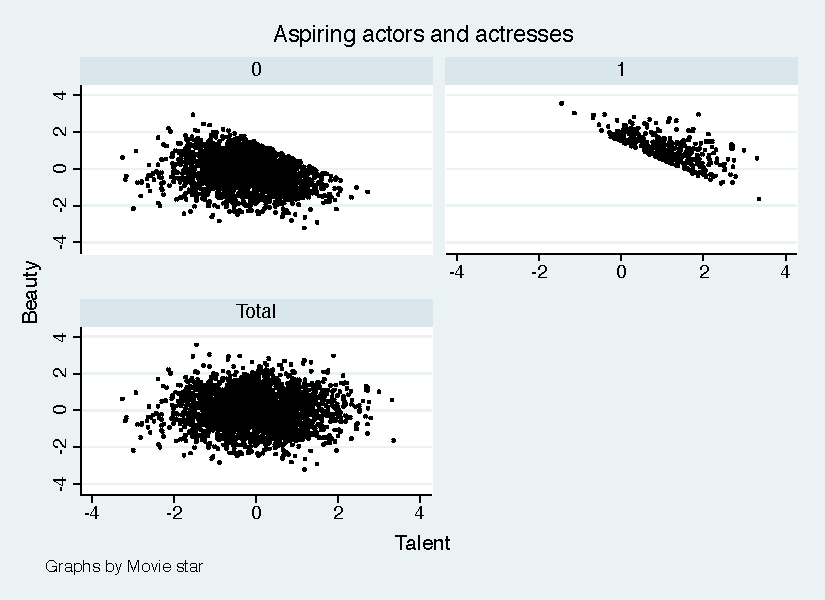
\includegraphics[height=9cm]{./lecture_includes/beauty_collider.pdf}
    \caption{Top left figure: Non-star sample scatter plot of beauty (vertical axis) and talent (horizontal axis). Top right right figure: Star sample scatter plot of beauty and talent.  Bottom left figure: Entire (stars and non-stars combined) sample scatter plot of beauty and talent.}
  \end{figure}
\end{frame}

\begin{frame}{Sample selection?}

\begin{itemize}
\item Notice that this is clear when we are focused on sample selection
\item But even a regression that included ``star'' would create the issue:$$beauty_i = \alpha + \delta talent_i + \beta star_i + \varepsilon_i$$
\item It's not just sample selection 
\end{itemize}

\end{frame}


\begin{frame}{Example 2: Discrimination}

  \begin{itemize}
    \item Let's look at another example: very common for think tanks and journalists to say that the gender gap in earnings disappears once you control for occupation.
    \item But what if occupation is a collider, which it could be in a model with occupational sorting
    \item Then controlling for occupation in a wage regression searching for discrimination can lead to all kinds of crazy results \emph{even in a simulation where we explicitly design there to be discrimination}
  \end{itemize}

\end{frame}

\begin{frame}{DAG}

  \begin{center}
    \begin{tikzpicture}
      [node distance=1.5cm]
      % nodes %
      \node[text centered] (f) {$F$};
      \node[above right of = f, text centered] (d) {$d$};
      \node[right of = f] (y) {$y$};
      \node[below  of = f, text centered] (o) {$o$};
      \node[right of = o, text centered] (a) {$A$};

      % edges %
      \draw[->, line width= 1] (f) -- (d);
      \draw[->, line width= 1] (d) -- (o);
      \draw[->, line width= 1, dashed] (a) -- (o);

      \draw[->, line width= 1] (d) -- (y);
      \draw[->, line width= 1] (o) -- (y);
      \draw[->, line width= 1, dashed] (a) -- (y);

    \end{tikzpicture}
  \end{center}

  $F$ is female, $d$ is discrimination, $o$ is occupation, $y$ is earnings and $A$ is ability. Dashed lines mean the variable cannot be observed. Note, by design, being a female has no effect on earnings or occupation, and has no relationship with ability. So earnings is coming through discrimination, occupation, and ability.

\end{frame}


\begin{frame}[plain]

  \begin{center}
    \begin{tikzpicture}
      [node distance=1.5cm]
      % nodes %
      \node[text centered] (f) {$F$};
      \node[above right of = f, text centered] (d) {$d$};
      \node[right of = f] (y) {$y$};
      \node[below  of = f, text centered] (o) {$o$};
      \node[right of = o, text centered] (a) {$A$};

      % edges %
      \draw[->, line width= 1] (f) -- (d);
      \draw[->, line width= 1] (d) -- (o);
      \draw[->, line width= 1, dashed] (a) -- (o);

      \draw[->, line width= 1] (d) -- (y);
      \draw[->, line width= 1] (o) -- (y);
      \draw[->, line width= 1, dashed] (a) -- (y);

    \end{tikzpicture}
  \end{center}


  Mediation and Backdoor paths

  \begin{enumerate}

    \item $d$ $\rightarrow o \rightarrow y$
    \item $d$ $\rightarrow o \leftarrow A \rightarrow y$
  \end{enumerate}

\end{frame}


\begin{frame}[plain, shrink=20]

  \begin{table}[htbp]\centering
    \scriptsize
    \caption{Regressions illustrating collider bias with simulated gender disparity}
    \begin{center}
      \begin{tabular}{l*{3}{c}}
        \toprule
        \multicolumn{1}{l}{Covariates: }&
        \multicolumn{1}{c}{\textbf{Unbiased combined effect}}&
        \multicolumn{1}{c}{\textbf{Biased }}&
        \multicolumn{1}{c}{\textbf{Unbiased wage effect only}}\\
        \midrule
        Female                     & -3.074*** & 0.601*** & -0.994*** \\
                                   & (0.000)   & (0.000)  & (0.000)   \\
        Occupation                 &           & 1.793*** & 0.991***  \\
                                   &           & (0.000)  & (0.000)   \\
        Ability                    &           &          & 2.017***  \\
                                   &           &          & (0.000)   \\
        \\
        \midrule
        N                          & 10,000    & 10,000   & 10,000    \\
        Mean of dependent variable & 0.45      & 0.45     & 0.45      \\
        \bottomrule
      \end{tabular}
    \end{center}
  \end{table}

  \begin{itemize}
    \item Recall we designed there to be a discrimination coefficient of -1
    \item If we do not control for occupation, then we get the combined effect of $d \rightarrow o \rightarrow y$ and $d  \rightarrow y$
    \item Because it seems intuitive to control for occupation, notice column 2 - the sign flips!
    \item We are only able to isolate the direct causal effect by conditioning on ability and occupation, but ability is unobserved
  \end{itemize}

\end{frame}

\begin{frame}[allowframebreaks,plain]

  \begin{itemize}
    \item \textbf{Colliders can be outcomes (and often those are the ones)}
          \begin{itemize}
            \item There is only one backdoor path from $D$ to $Y$

                  \begin{center}
                    \begin{tikzpicture}
                      [node distance=1.5cm]
                      % nodes %
                      \node[text centered,draw,rectangle,thin] (x1) {$X_1$};
                      \node[right of = x1, text centered] (d) {$D$};
                      \node[below right of = d, text centered] (x2) {$X_2$};
                      \node[above right of = x2, text centered] (y) {$Y$};

                      % edges %
                      \draw[->, line width= .5] (x1) -- (d);
                      \draw[->, line width= .5] (d) -- (y);
                      \draw[->, line width= .5] (d) -- (x2);
                      \draw[->, line width= .5] (y) -- (x2);
                      \draw[->, line width= .5] (x1) to [out=45,in=135, looseness=0.5] (y);
                    \end{tikzpicture}
                  \end{center}
                  

            \item Conditioning on $X_1$ blocks the backdoor path


            \item But what if we also condition on $X_2$?

                  \begin{center}
                    \begin{tikzpicture}
                      [node distance=1.5cm]
                      % nodes %
                      \node[text centered,draw,rectangle,thin] (x1) {$X_1$};
                      \node[right of = x1, text centered] (d) {$D$};
                      \node[below right of = d, draw, rectangle, text centered] (x2) {$X_2$};
                      \node[above right of = x2, text centered] (y) {$Y$};

                      % edges %
                      \draw[->, line width= .5] (x1) -- (d);
                      \draw[->, line width= .5] (d) -- (y);
                      \draw[->, line width= .5] (d) -- (x2);
                      \draw[->, line width= .5] (y) -- (x2);
                      \draw[->, line width= .5] (x1) to [out=45,in=135, looseness=0.5] (y);
                    \end{tikzpicture}
                  \end{center}

            \item Conditioning on $X_2$ opens up a new path, creating new spurious correlations between $D$ and $Y$ 
          \end{itemize}

          \framebreak


    \item \textbf{Colliders could be pre-treatment covariates (called M-bias because it looks like an M)}
          \begin{itemize}
            \item Name the backdoor paths.  Is it open or closed?

                  \begin{center}
                    \begin{tikzpicture}
                      [node distance=1.5cm, text centered]
                      % nodes %
                      \node[] (x) {$X$};
                      \node[above left of = x] (u1) {$U_1$};
                      \node[below left of = x] (u2) {$U_2$};
                      \node[right of = x] (d) {$D$};
                      \node[right of = d] (y) {$Y$};

                      % edges %
                      \draw[->, line width= .5, dashed] (u1) -- (x);
                      \draw[->, line width= .5, dashed] (u2) -- (x);
                      \draw[->, line width= .5, dashed] (u1) to [out=0,in=135, looseness=0.5] (y);
                      \draw[->, line width= .5, dashed] (u2) to [out=0,in=-135, looseness=0.5] (d);
                      \draw[->, line width= .5] (d) -- (y);
                    \end{tikzpicture}
                  \end{center}

            \item But what if we condition on $X$?

                  \begin{center}
                    \begin{tikzpicture}
                      [node distance=1.5cm, text centered]
                      % nodes %
                      \node[text centered,draw,rectangle,thin] (x) {$X$};
                      \node[above left of = x] (u1) {$U_1$};
                      \node[below left of = x] (u2) {$U_2$};
                      \node[right of = x] (d) {$D$};
                      \node[right of = d] (y) {$Y$};

                      % edges %
                      \draw[->, line width= .5, dashed] (u1) -- (x);
                      \draw[->, line width= .5, dashed] (u2) -- (x);
                      \draw[->, line width= .5, dashed] (u1) to [out=0,in=135, looseness=0.5] (y);
                      \draw[->, line width= .5, dashed] (u2) to [out=0,in=-135, looseness=0.5] (d);
                      \draw[->, line width= .5] (d) -- (y);
                    \end{tikzpicture}
                  \end{center}


          \end{itemize}
  \end{itemize}
  \framebreak


\end{frame}


\begin{frame}{M-bias as collider}

  \centering
  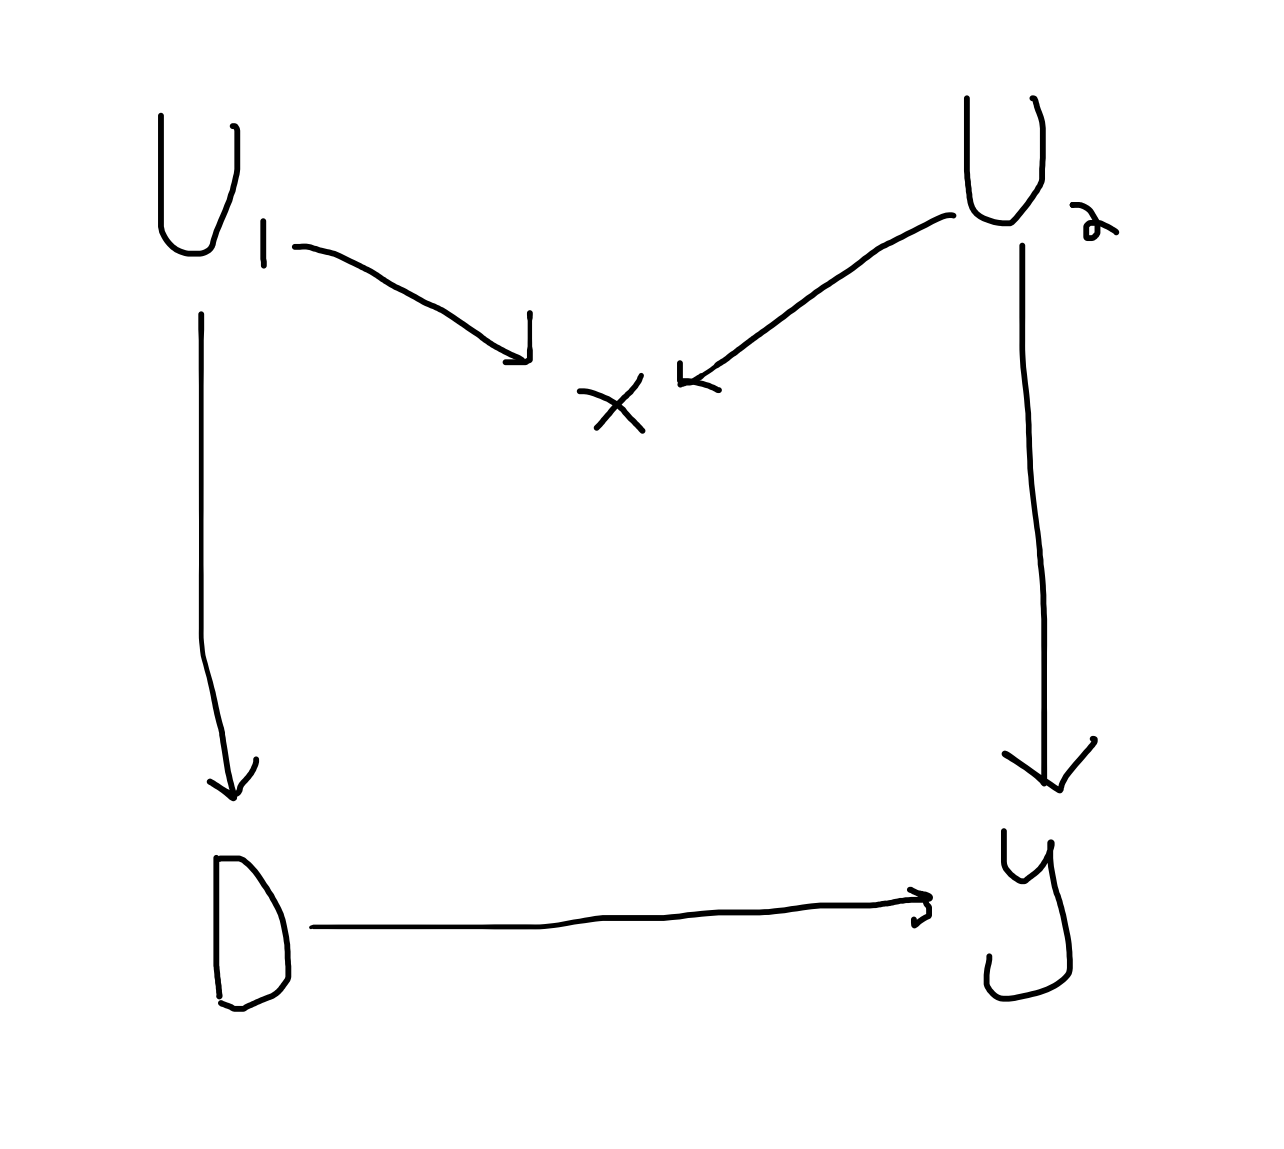
\includegraphics[height=5.8cm, width=10cm]{./lecture_includes/mbias}

\footnotesize
$X$ is pre-treatment, but if you conditioned on it, then $D\leftarrow U1 \rightarrow \mbox{X} \leftarrow U2 \rightarrow Y$ and $X$ is a collider. Colliders take strange forms, so the conditioning set \emph{must} be thoughtfully chosen based on being a strong predictor of $Y^0$, preferably based on expert knowledge and not a kitchen sink of all available regressors

\end{frame}


\begin{frame}{Testing the Validity of the DAG}

  \begin{itemize}
    \item The DAG makes testable predictions
    \item Conditional on $D$ and $I$, parental education ($PE$) should no longer be correlated with $Y$
    \item Can be hard to figure this out by hand, but software can help (e.g., Daggity.net is browser based, Causal Fusion is more advanced)
    \item Causal algorithms tend to be DAG based and are becoming popular in industry 
  \end{itemize}

  \begin{center}
    \begin{tikzpicture}[node distance=1.5cm]
      % nodes %
      \node[text centered] (d) {$D$};
      \node[right of = d, text centered] (y) {$Y$};
      \node[above left of = d, text centered] (i) {$I$};
      \node[left of = i, text centered] (pe) {$PE$};
      \node[below of = pe, text centered] (b) {$B$};
      % edges %
      \draw[->, line width= 1] (d) -- (y);
      \draw[->, line width= 1,] (i) -- (d);
      \draw[->, line width= 1,] (pe) -- (i);
      \draw[->, line width= 1,] (pe) -- (d);
      \draw[->, line width= 1, dashed] (b) -- (pe);
      \draw[->, line width= 1, dashed] (b) -- (d);
      \draw[->, line width= .5] (i) to [out=45,in=135, looseness=0.5] (y);
    \end{tikzpicture}
  \end{center}

\end{frame}




\begin{frame}{Contrast this with ordinary practices}

\begin{itemize}
\item Person attempts to ``control for omitted variable bias'' by including as many ``controls'' as possible
\item Person does not even attempt to think about treatment assignment mechanism and therefore has no idea what variables are colliders, covariates or confounders
\item Machine learning can be ``naive'' too if the large dimension of features includes unknowingly colliders
\end{itemize}

\end{frame}

\begin{frame}{}

  \begin{figure}
    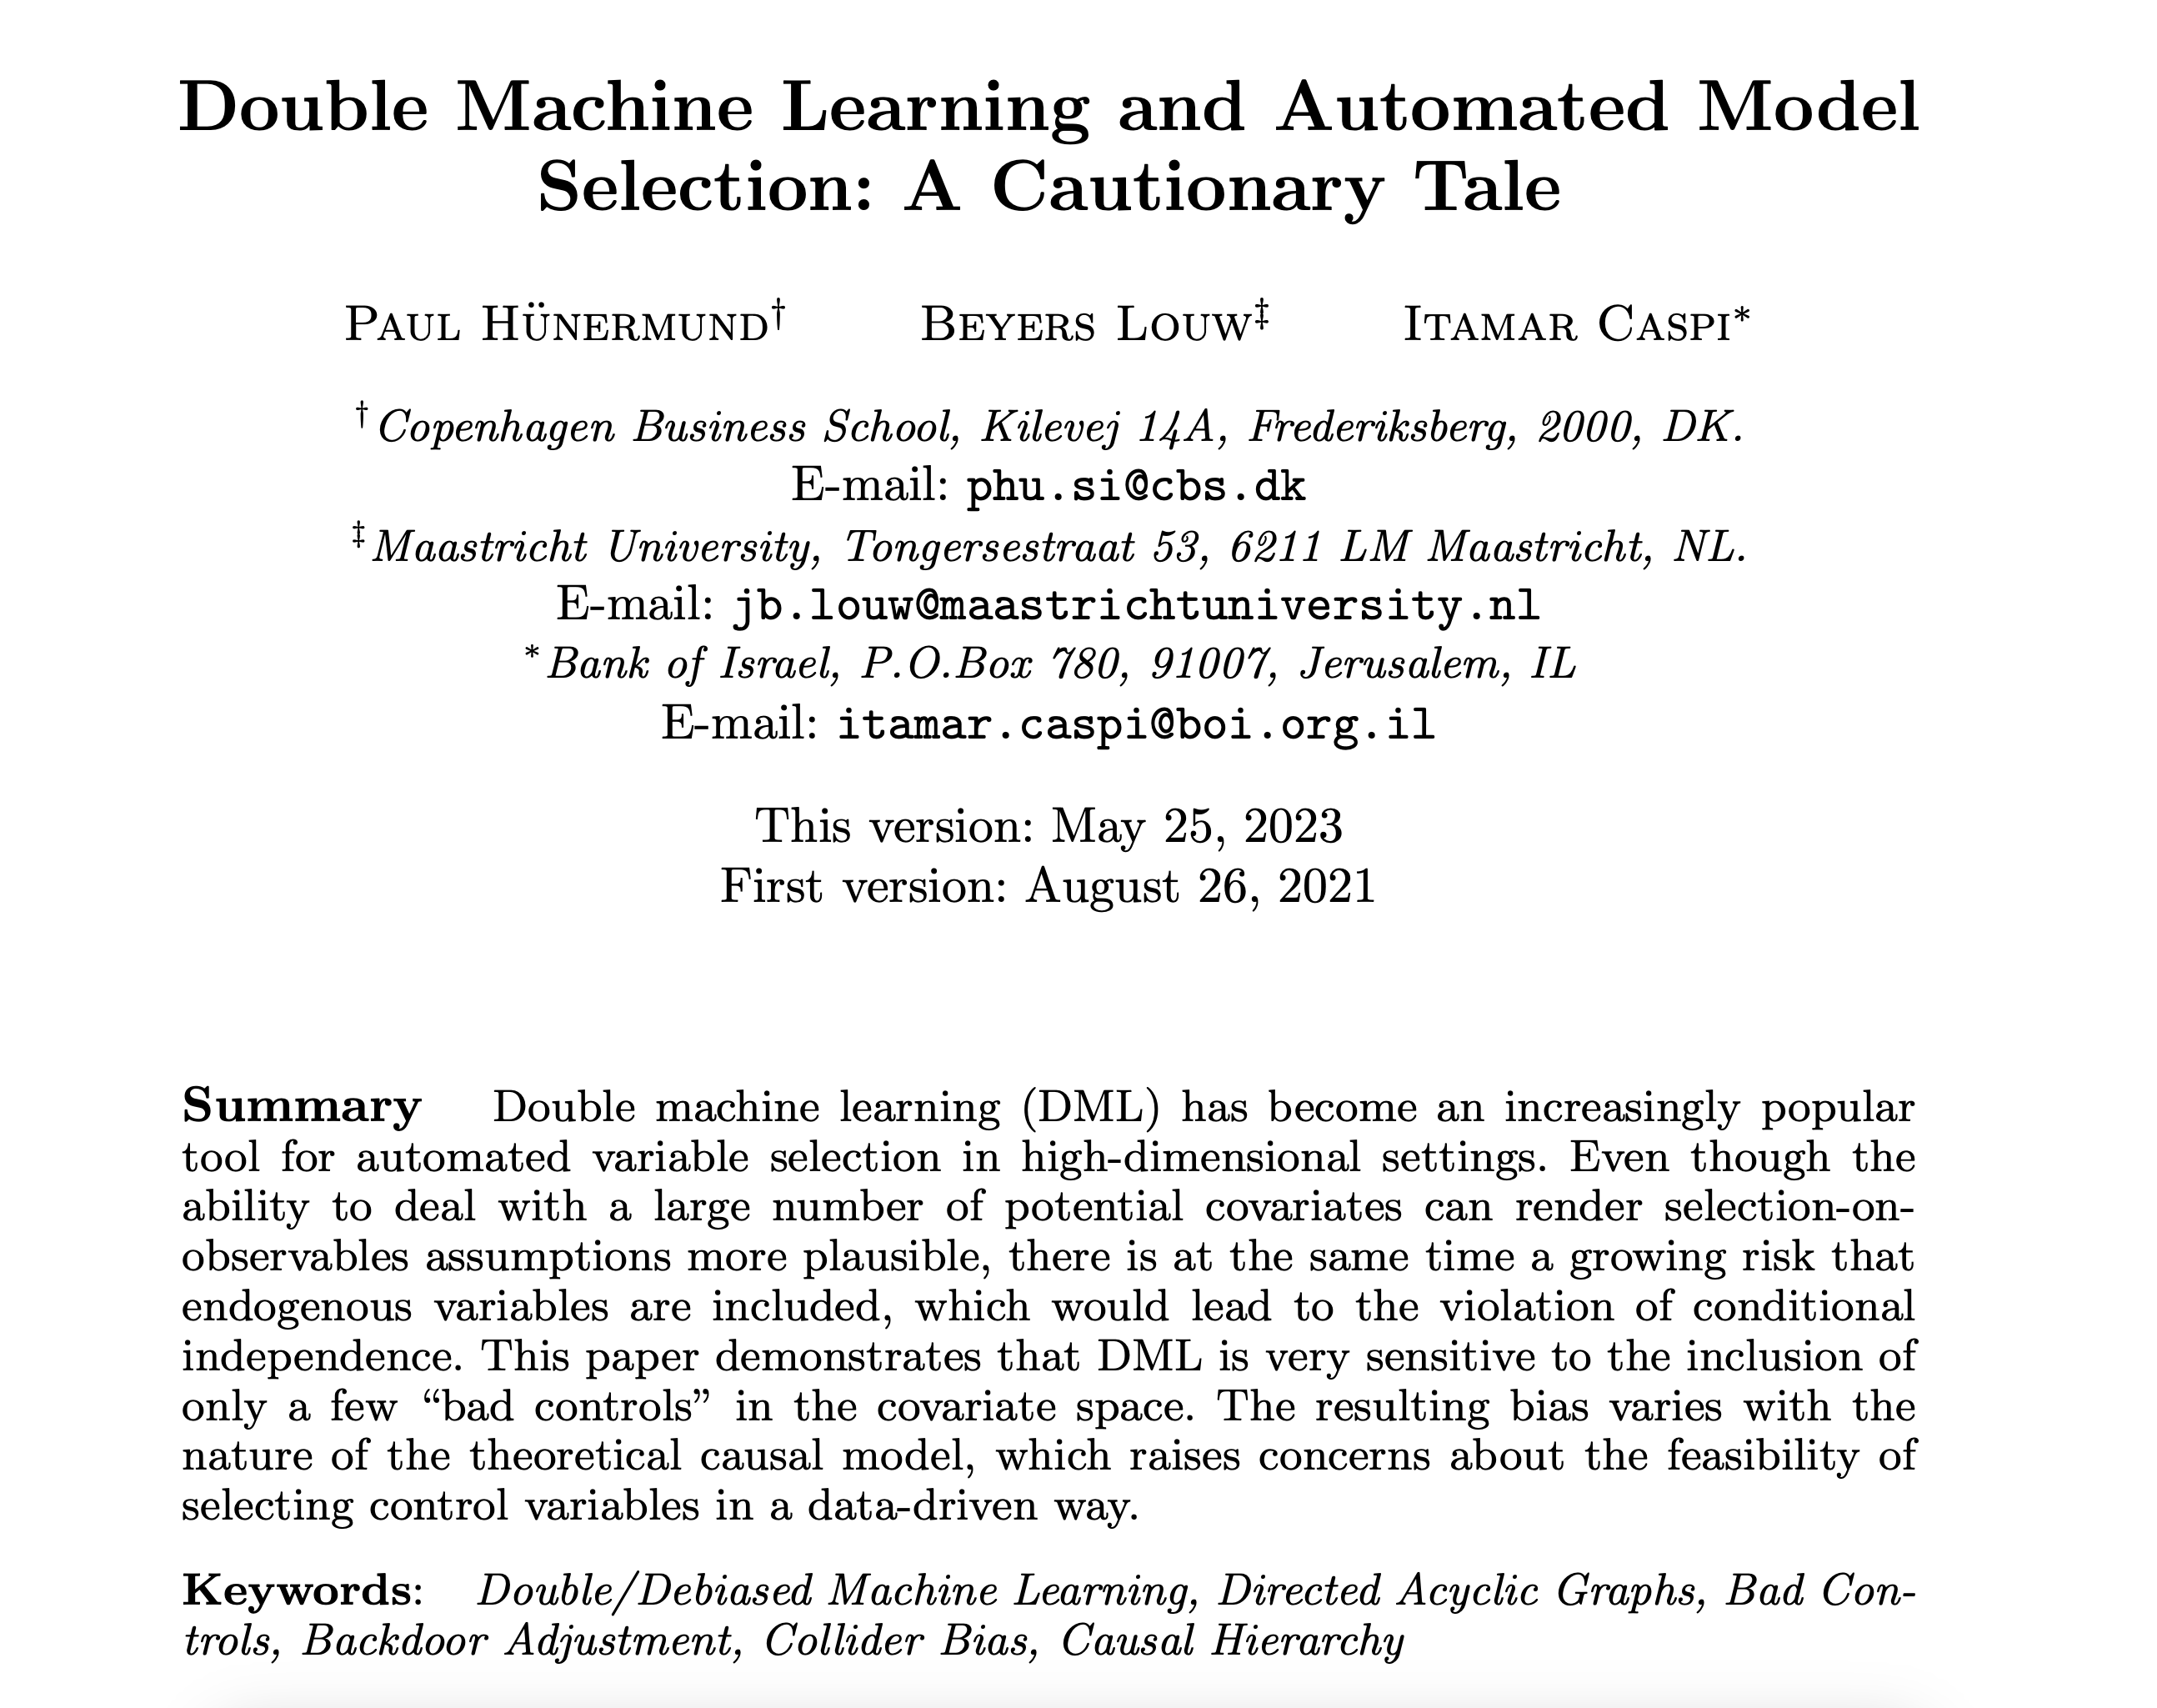
\includegraphics[scale=0.25]{./lecture_includes/paul_dml}
  \end{figure}

\end{frame}




\begin{frame}{Covariate selection without DAGs}

\begin{itemize}
\item What if you don't have a DAG you feel confident about?  
	\begin{enumerate}
	\item Include confounders that you feel pretty confident are there 
	\item Include covariates that are \emph{highly predictive} of the missing counterfactual (e.g., $Y^0$ for the ATT)
	\item Avoid outcomes (even though that still won't address M-bias colliders)
	\end{enumerate}
\item While this approach may be less formalized, you are at least reasoning about the treatment assignment mechanism as opposed to just including whatever variables you have laying around (avoid the ``kitchen sink regressions'')
\end{itemize}

\end{frame}

\begin{frame}{Falsifications as a test}

\begin{itemize}
\item Covariates should not be affected by the treatment, so examining them as falsifications can help establish the credibility of unconfoundedness
\item Imbens and Rubin (2015) suggested using the lagged outcome (pre-treatment) as a way of checking, as those have similar confounder structures
\item Falsifications too: One study questioned a finding that obesity was contagious in social networks by estimating the same model on things that cannot be contagious like acne, headaches and height and found the same things (likely confounding existed)
\end{itemize}

\end{frame}




